\documentclass[twoside]{book}

% Packages required by doxygen
\usepackage{fixltx2e}
\usepackage{calc}
\usepackage{doxygen}
\usepackage[export]{adjustbox} % also loads graphicx
\usepackage{graphicx}
\usepackage[utf8]{inputenc}
\usepackage{makeidx}
\usepackage{multicol}
\usepackage{multirow}
\PassOptionsToPackage{warn}{textcomp}
\usepackage{textcomp}
\usepackage[nointegrals]{wasysym}
\usepackage[table]{xcolor}

% Font selection
\usepackage[T1]{fontenc}
\usepackage[scaled=.90]{helvet}
\usepackage{courier}
\usepackage{amssymb}
\usepackage{sectsty}
\renewcommand{\familydefault}{\sfdefault}
\allsectionsfont{%
  \fontseries{bc}\selectfont%
  \color{darkgray}%
}
\renewcommand{\DoxyLabelFont}{%
  \fontseries{bc}\selectfont%
  \color{darkgray}%
}
\newcommand{\+}{\discretionary{\mbox{\scriptsize$\hookleftarrow$}}{}{}}

% Page & text layout
\usepackage{geometry}
\geometry{%
  a4paper,%
  top=2.5cm,%
  bottom=2.5cm,%
  left=2.5cm,%
  right=2.5cm%
}
\tolerance=750
\hfuzz=15pt
\hbadness=750
\setlength{\emergencystretch}{15pt}
\setlength{\parindent}{0cm}
\setlength{\parskip}{3ex plus 2ex minus 2ex}
\makeatletter
\renewcommand{\paragraph}{%
  \@startsection{paragraph}{4}{0ex}{-1.0ex}{1.0ex}{%
    \normalfont\normalsize\bfseries\SS@parafont%
  }%
}
\renewcommand{\subparagraph}{%
  \@startsection{subparagraph}{5}{0ex}{-1.0ex}{1.0ex}{%
    \normalfont\normalsize\bfseries\SS@subparafont%
  }%
}
\makeatother

% Headers & footers
\usepackage{fancyhdr}
\pagestyle{fancyplain}
\fancyhead[LE]{\fancyplain{}{\bfseries\thepage}}
\fancyhead[CE]{\fancyplain{}{}}
\fancyhead[RE]{\fancyplain{}{\bfseries\leftmark}}
\fancyhead[LO]{\fancyplain{}{\bfseries\rightmark}}
\fancyhead[CO]{\fancyplain{}{}}
\fancyhead[RO]{\fancyplain{}{\bfseries\thepage}}
\fancyfoot[LE]{\fancyplain{}{}}
\fancyfoot[CE]{\fancyplain{}{}}
\fancyfoot[RE]{\fancyplain{}{\bfseries\scriptsize Generated by Doxygen }}
\fancyfoot[LO]{\fancyplain{}{\bfseries\scriptsize Generated by Doxygen }}
\fancyfoot[CO]{\fancyplain{}{}}
\fancyfoot[RO]{\fancyplain{}{}}
\renewcommand{\footrulewidth}{0.4pt}
\renewcommand{\chaptermark}[1]{%
  \markboth{#1}{}%
}
\renewcommand{\sectionmark}[1]{%
  \markright{\thesection\ #1}%
}

% Indices & bibliography
\usepackage{natbib}
\usepackage[titles]{tocloft}
\setcounter{tocdepth}{3}
\setcounter{secnumdepth}{5}
\makeindex

% Hyperlinks (required, but should be loaded last)
\usepackage{ifpdf}
\ifpdf
  \usepackage[pdftex,pagebackref=true]{hyperref}
\else
  \usepackage[ps2pdf,pagebackref=true]{hyperref}
\fi
\hypersetup{%
  colorlinks=true,%
  linkcolor=blue,%
  citecolor=blue,%
  unicode%
}

% Custom commands
\newcommand{\clearemptydoublepage}{%
  \newpage{\pagestyle{empty}\cleardoublepage}%
}

\usepackage{caption}
\captionsetup{labelsep=space,justification=centering,font={bf},singlelinecheck=off,skip=4pt,position=top}

%===== C O N T E N T S =====

\begin{document}

% Titlepage & ToC
\hypersetup{pageanchor=false,
             bookmarksnumbered=true,
             pdfencoding=unicode
            }
\pagenumbering{alph}
\begin{titlepage}
\vspace*{7cm}
\begin{center}%
{\Large Antitelephone \\[1ex]\large 0.\+1 }\\
\vspace*{1cm}
{\large Generated by Doxygen 1.8.13}\\
\end{center}
\end{titlepage}
\clearemptydoublepage
\pagenumbering{roman}
\tableofcontents
\clearemptydoublepage
\pagenumbering{arabic}
\hypersetup{pageanchor=true}

%--- Begin generated contents ---
\chapter{Index}
\label{index}\hypertarget{index}{}This project is a new concept for a multiplayer time travel game inspired by the parallel universe theory. For more information about the game, visit the \href{https://github.com/JubilantJerry/Antitelephone}{\tt Git\+Hub repository}.

This page contains the documentation of the classes used in the game. In general, documentation is limited to header files. 
\chapter{Hierarchical Index}
\section{Class Hierarchy}
This inheritance list is sorted roughly, but not completely, alphabetically\+:\begin{DoxyCompactList}
\item \contentsline{section}{item\+:\+:Effect}{\pageref{classitem_1_1_effect}}{}
\item \contentsline{section}{std\+:\+:hash$<$ timeplane\+:\+:Moment $>$}{\pageref{structstd_1_1hash_3_01timeplane_1_1_moment_01_4}}{}
\item \contentsline{section}{item\+:\+:Item}{\pageref{classitem_1_1_item}}{}
\begin{DoxyCompactList}
\item \contentsline{section}{item\+:\+:Antitelephone}{\pageref{classitem_1_1_antitelephone}}{}
\item \contentsline{section}{item\+:\+:Bridge}{\pageref{classitem_1_1_bridge}}{}
\item \contentsline{section}{item\+:\+:Oracle}{\pageref{classitem_1_1_oracle}}{}
\item \contentsline{section}{item\+:\+:Shield}{\pageref{classitem_1_1_shield}}{}
\end{DoxyCompactList}
\item \contentsline{section}{item\+:\+:Item\+Properties}{\pageref{classitem_1_1_item_properties}}{}
\item \contentsline{section}{timeplane\+:\+:Moment}{\pageref{classtimeplane_1_1_moment}}{}
\item \contentsline{section}{roundinfo\+:\+:Round\+Info}{\pageref{classroundinfo_1_1_round_info}}{}
\item \contentsline{section}{roundinfo\+:\+:Round\+Info\+View}{\pageref{classroundinfo_1_1_round_info_view}}{}
\item \contentsline{section}{Symmetric\+Bit\+Matrix}{\pageref{class_symmetric_bit_matrix}}{}
\item \contentsline{section}{timeplane\+:\+:Time\+Line}{\pageref{classtimeplane_1_1_time_line}}{}
\item \contentsline{section}{timeplane\+:\+:Time\+Plane}{\pageref{classtimeplane_1_1_time_plane}}{}
\end{DoxyCompactList}

\chapter{Class Index}
\section{Class List}
Here are the classes, structs, unions and interfaces with brief descriptions\+:\begin{DoxyCompactList}
\item\contentsline{section}{\hyperlink{classitem_1_1_antitelephone}{item\+::\+Antitelephone} \\*\hyperlink{classitem_1_1_item}{Item} which allows traveling to the past }{\pageref{classitem_1_1_antitelephone}}{}
\item\contentsline{section}{\hyperlink{classitem_1_1_bridge}{item\+::\+Bridge} \\*\hyperlink{classitem_1_1_item}{Item} which bridges together separated moments }{\pageref{classitem_1_1_bridge}}{}
\item\contentsline{section}{\hyperlink{classitem_1_1_effect}{item\+::\+Effect} }{\pageref{classitem_1_1_effect}}{}
\item\contentsline{section}{\hyperlink{structstd_1_1hash_3_01timeplane_1_1_moment_01_4}{std\+::hash$<$ timeplane\+::\+Moment $>$} \\*Hash function for {\ttfamily Moment} instances }{\pageref{structstd_1_1hash_3_01timeplane_1_1_moment_01_4}}{}
\item\contentsline{section}{\hyperlink{classitem_1_1_item}{item\+::\+Item} \\*The properties of an item in the game across moments }{\pageref{classitem_1_1_item}}{}
\item\contentsline{section}{\hyperlink{classitem_1_1_item_properties}{item\+::\+Item\+Properties} \\*A class holding properties of an item at a specific moment }{\pageref{classitem_1_1_item_properties}}{}
\item\contentsline{section}{\hyperlink{classtimeplane_1_1_moment}{timeplane\+::\+Moment} \\*A unique moment in a {\ttfamily \hyperlink{classtimeplane_1_1_time_plane}{Time\+Plane}} }{\pageref{classtimeplane_1_1_moment}}{}
\item\contentsline{section}{\hyperlink{classitem_1_1_oracle}{item\+::\+Oracle} \\*\hyperlink{classitem_1_1_item}{Item} that can make a player controllable }{\pageref{classitem_1_1_oracle}}{}
\item\contentsline{section}{\hyperlink{classroundinfo_1_1_round_info}{roundinfo\+::\+Round\+Info} \\*A representation of data relevant to a single round of gameplay }{\pageref{classroundinfo_1_1_round_info}}{}
\item\contentsline{section}{\hyperlink{classroundinfo_1_1_round_info_view}{roundinfo\+::\+Round\+Info\+View} \\*Information contained in {\ttfamily \hyperlink{classroundinfo_1_1_round_info}{Round\+Info}} as seen from a single player }{\pageref{classroundinfo_1_1_round_info_view}}{}
\item\contentsline{section}{\hyperlink{classitem_1_1_shield}{item\+::\+Shield} \\*\hyperlink{classitem_1_1_item}{Item} that shields that player from damage }{\pageref{classitem_1_1_shield}}{}
\item\contentsline{section}{\hyperlink{class_symmetric_bit_matrix}{Symmetric\+Bit\+Matrix} \\*A symmetric square matrix of boolean values }{\pageref{class_symmetric_bit_matrix}}{}
\item\contentsline{section}{\hyperlink{classtimeplane_1_1_time_line}{timeplane\+::\+Time\+Line} \\*A chronological sequence of {\ttfamily \hyperlink{classtimeplane_1_1_moment}{Moment}} instances }{\pageref{classtimeplane_1_1_time_line}}{}
\item\contentsline{section}{\hyperlink{classtimeplane_1_1_time_plane}{timeplane\+::\+Time\+Plane} \\*A wrapper to access individual {\ttfamily \hyperlink{classtimeplane_1_1_time_line}{Time\+Line}} instances }{\pageref{classtimeplane_1_1_time_plane}}{}
\end{DoxyCompactList}

\chapter{Class Documentation}
\hypertarget{classitem_1_1_antitelephone}{}\section{item\+:\+:Antitelephone Class Reference}
\label{classitem_1_1_antitelephone}\index{item\+::\+Antitelephone@{item\+::\+Antitelephone}}


\hyperlink{classitem_1_1_item}{Item} which allows traveling to the past.  




{\ttfamily \#include $<$antitelephone.\+hpp$>$}

Inheritance diagram for item\+:\+:Antitelephone\+:\begin{figure}[H]
\begin{center}
\leavevmode
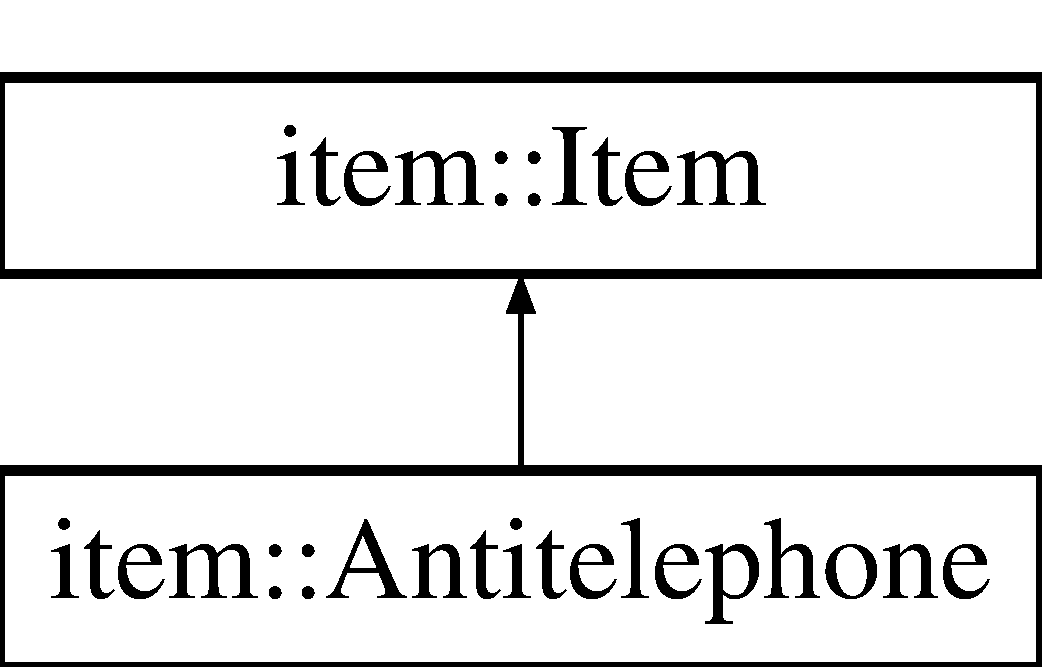
\includegraphics[height=2.000000cm]{classitem_1_1_antitelephone}
\end{center}
\end{figure}
\subsection*{Public Member Functions}
\begin{DoxyCompactItemize}
\item 
\mbox{\Hypertarget{classitem_1_1_antitelephone_a832d79223e555ae7dd69d11377392731}\label{classitem_1_1_antitelephone_a832d79223e555ae7dd69d11377392731}} 
{\bfseries Antitelephone} (\hyperlink{classtimeplane_1_1_moment}{Moment} first\+\_\+moment)
\item 
\hyperlink{classitem_1_1_effect}{Effect} \hyperlink{classitem_1_1_antitelephone_ae8f9abbbb65d23970fb3b61393bda141}{View} (\hyperlink{classtimeplane_1_1_moment}{Moment}) const
\begin{DoxyCompactList}\small\item\em View the effects of an item at a specific moment. \end{DoxyCompactList}\item 
Tagged\+Values \hyperlink{classitem_1_1_antitelephone_afe8ac703b5f19181f221afe07c05cae7}{State\+Tagged\+Values} (\hyperlink{classtimeplane_1_1_moment}{Moment} m) const
\begin{DoxyCompactList}\small\item\em Virtual method to provide user-\/friendly tagged values. \end{DoxyCompactList}\end{DoxyCompactItemize}
\subsection*{Static Public Attributes}
\begin{DoxyCompactItemize}
\item 
static Item\+Type constexpr \hyperlink{classitem_1_1_antitelephone_ab6d34885da8ab27a578da87a0c746744}{type} = Item\+Type\+::k\+Antitelephone
\begin{DoxyCompactList}\small\item\em An enum representation of the type of the item. \end{DoxyCompactList}\end{DoxyCompactItemize}
\subsection*{Protected Member Functions}
\begin{DoxyCompactItemize}
\item 
std\+::pair$<$ \hyperlink{classitem_1_1_effect}{Effect}, \hyperlink{classitem_1_1_item_properties}{Item\+Properties} $>$ \hyperlink{classitem_1_1_antitelephone_aa59b4569bac948f37fd15dbea234503f}{Step\+Impl} (\hyperlink{classtimeplane_1_1_moment}{Moment} curr, \hyperlink{classroundinfo_1_1_round_info_view}{Round\+Info\+View} const \&round\+\_\+info\+\_\+view, int energy\+\_\+input)
\begin{DoxyCompactList}\small\item\em Virtual method for computing the results of making a step. \end{DoxyCompactList}\item 
std\+::pair$<$ \hyperlink{classitem_1_1_effect}{Effect}, \hyperlink{classitem_1_1_item_properties}{Item\+Properties} $>$ \hyperlink{classitem_1_1_antitelephone_a1b094baeb7cae7e1161d1aa1650022d1}{Branch\+Impl} (\hyperlink{classtimeplane_1_1_moment}{Moment} curr, \hyperlink{classtimeplane_1_1_moment}{Moment} dest)
\begin{DoxyCompactList}\small\item\em Virtual method for computing the results of branching. \end{DoxyCompactList}\end{DoxyCompactItemize}
\subsection*{Additional Inherited Members}


\subsection{Detailed Description}
\hyperlink{classitem_1_1_item}{Item} which allows traveling to the past. 

\subsection{Member Function Documentation}
\mbox{\Hypertarget{classitem_1_1_antitelephone_ae8f9abbbb65d23970fb3b61393bda141}\label{classitem_1_1_antitelephone_ae8f9abbbb65d23970fb3b61393bda141}} 
\index{item\+::\+Antitelephone@{item\+::\+Antitelephone}!View@{View}}
\index{View@{View}!item\+::\+Antitelephone@{item\+::\+Antitelephone}}
\subsubsection{\texorpdfstring{View()}{View()}}
{\footnotesize\ttfamily \hyperlink{classitem_1_1_effect}{Effect} Antitelephone\+::\+View (\begin{DoxyParamCaption}\item[{\hyperlink{classtimeplane_1_1_moment}{Moment}}]{m }\end{DoxyParamCaption}) const\hspace{0.3cm}{\ttfamily [virtual]}}



View the effects of an item at a specific moment. 

This call must be a pure function not only of the provided moment, but also be a function of {\ttfamily Get\+Properties(m)}. 
\begin{DoxyParams}{Parameters}
{\em m} & The moment to query. \\
\hline
\end{DoxyParams}
\begin{DoxyReturn}{Returns}
The effects granted by the item at the specified moment. 
\end{DoxyReturn}

\begin{DoxyExceptions}{Exceptions}
{\em std\+::out\+\_\+of\+\_\+range} & Potentially thrown by subclasses. \\
\hline
\end{DoxyExceptions}


Implements \hyperlink{classitem_1_1_item_a7d2b010a27fec55e04a56e7c4fca7837}{item\+::\+Item}.

\mbox{\Hypertarget{classitem_1_1_antitelephone_afe8ac703b5f19181f221afe07c05cae7}\label{classitem_1_1_antitelephone_afe8ac703b5f19181f221afe07c05cae7}} 
\index{item\+::\+Antitelephone@{item\+::\+Antitelephone}!State\+Tagged\+Values@{State\+Tagged\+Values}}
\index{State\+Tagged\+Values@{State\+Tagged\+Values}!item\+::\+Antitelephone@{item\+::\+Antitelephone}}
\subsubsection{\texorpdfstring{State\+Tagged\+Values()}{StateTaggedValues()}}
{\footnotesize\ttfamily Tagged\+Values Antitelephone\+::\+State\+Tagged\+Values (\begin{DoxyParamCaption}\item[{\hyperlink{classtimeplane_1_1_moment}{Moment}}]{m }\end{DoxyParamCaption}) const\hspace{0.3cm}{\ttfamily [virtual]}}



Virtual method to provide user-\/friendly tagged values. 

The tags are used as a user-\/friendly indication of the internal state of the item at a given moment without revealing implementation detail, and can also be used to attach specific meaning to the abstract lockdown and cooldown values associated with all items. 
\begin{DoxyParams}{Parameters}
{\em m} & The moment to query. \\
\hline
\end{DoxyParams}
\begin{DoxyReturn}{Returns}
A group of tagged values describing the state of an item. 
\end{DoxyReturn}


Implements \hyperlink{classitem_1_1_item_a8410ab3ab75e65360eddb4f6bd3cceff}{item\+::\+Item}.

\mbox{\Hypertarget{classitem_1_1_antitelephone_aa59b4569bac948f37fd15dbea234503f}\label{classitem_1_1_antitelephone_aa59b4569bac948f37fd15dbea234503f}} 
\index{item\+::\+Antitelephone@{item\+::\+Antitelephone}!Step\+Impl@{Step\+Impl}}
\index{Step\+Impl@{Step\+Impl}!item\+::\+Antitelephone@{item\+::\+Antitelephone}}
\subsubsection{\texorpdfstring{Step\+Impl()}{StepImpl()}}
{\footnotesize\ttfamily std\+::pair$<$ \hyperlink{classitem_1_1_effect}{Effect}, \hyperlink{classitem_1_1_item_properties}{Item\+Properties} $>$ Antitelephone\+::\+Step\+Impl (\begin{DoxyParamCaption}\item[{\hyperlink{classtimeplane_1_1_moment}{Moment}}]{curr,  }\item[{\hyperlink{classroundinfo_1_1_round_info_view}{Round\+Info\+View} const \&}]{turn\+\_\+data,  }\item[{int}]{energy\+\_\+input }\end{DoxyParamCaption})\hspace{0.3cm}{\ttfamily [protected]}, {\ttfamily [virtual]}}



Virtual method for computing the results of making a step. 


\begin{DoxyParams}{Parameters}
{\em curr} & The current moment before the step. \\
\hline
{\em turn\+\_\+data} & The information about the turn just played. \\
\hline
\end{DoxyParams}
\begin{DoxyReturn}{Returns}
The effects granted by the item for the next round, and the properties of the item for the next round. 
\end{DoxyReturn}


Implements \hyperlink{classitem_1_1_item_a90df61c8a2a20144eb1100af5fb2d464}{item\+::\+Item}.

\mbox{\Hypertarget{classitem_1_1_antitelephone_a1b094baeb7cae7e1161d1aa1650022d1}\label{classitem_1_1_antitelephone_a1b094baeb7cae7e1161d1aa1650022d1}} 
\index{item\+::\+Antitelephone@{item\+::\+Antitelephone}!Branch\+Impl@{Branch\+Impl}}
\index{Branch\+Impl@{Branch\+Impl}!item\+::\+Antitelephone@{item\+::\+Antitelephone}}
\subsubsection{\texorpdfstring{Branch\+Impl()}{BranchImpl()}}
{\footnotesize\ttfamily std\+::pair$<$ \hyperlink{classitem_1_1_effect}{Effect}, \hyperlink{classitem_1_1_item_properties}{Item\+Properties} $>$ Antitelephone\+::\+Branch\+Impl (\begin{DoxyParamCaption}\item[{\hyperlink{classtimeplane_1_1_moment}{Moment}}]{curr,  }\item[{\hyperlink{classtimeplane_1_1_moment}{Moment}}]{dest }\end{DoxyParamCaption})\hspace{0.3cm}{\ttfamily [protected]}, {\ttfamily [virtual]}}



Virtual method for computing the results of branching. 


\begin{DoxyParams}{Parameters}
{\em curr} & The current moment before branching. \\
\hline
{\em dest} & The destination moment to reach. \\
\hline
\end{DoxyParams}
\begin{DoxyReturn}{Returns}
The effects granted by the item for the next round, and the properties of the item for the next round. 
\end{DoxyReturn}


Implements \hyperlink{classitem_1_1_item_afef6bdd5c1c734c67122e4118e9e1930}{item\+::\+Item}.



\subsection{Member Data Documentation}
\mbox{\Hypertarget{classitem_1_1_antitelephone_ab6d34885da8ab27a578da87a0c746744}\label{classitem_1_1_antitelephone_ab6d34885da8ab27a578da87a0c746744}} 
\index{item\+::\+Antitelephone@{item\+::\+Antitelephone}!type@{type}}
\index{type@{type}!item\+::\+Antitelephone@{item\+::\+Antitelephone}}
\subsubsection{\texorpdfstring{type}{type}}
{\footnotesize\ttfamily Item\+Type constexpr item\+::\+Antitelephone\+::type = Item\+Type\+::k\+Antitelephone\hspace{0.3cm}{\ttfamily [static]}}



An enum representation of the type of the item. 

The value of the enum is a unique value for each item, and are consecutive starting at 0 across all items. 

The documentation for this class was generated from the following files\+:\begin{DoxyCompactItemize}
\item 
K\+:/\+Personal Projects/\+Antitelephone\+Q\+T/src/antitelephone.\+hpp\item 
K\+:/\+Personal Projects/\+Antitelephone\+Q\+T/src/antitelephone.\+cpp\end{DoxyCompactItemize}

\hypertarget{class_antitelephone_game}{}\section{Antitelephone\+Game Class Reference}
\label{class_antitelephone_game}\index{Antitelephone\+Game@{Antitelephone\+Game}}


Top level manager for Antitelephone internal game logic.  




{\ttfamily \#include $<$antitelephonegame.\+hpp$>$}

\subsection*{Public Types}
\begin{DoxyCompactItemize}
\item 
\mbox{\Hypertarget{class_antitelephone_game_a6f5bff3c072b992022d47276f2684848}\label{class_antitelephone_game_a6f5bff3c072b992022d47276f2684848}} 
using {\bfseries Time\+Plane} = \hyperlink{classtimeplane_1_1_time_plane}{timeplane\+::\+Time\+Plane}
\item 
\mbox{\Hypertarget{class_antitelephone_game_a8f68b4de9218b82ecfc9ebd24fc57813}\label{class_antitelephone_game_a8f68b4de9218b82ecfc9ebd24fc57813}} 
using {\bfseries Moment} = \hyperlink{classtimeplane_1_1_moment}{timeplane\+::\+Moment}
\item 
\mbox{\Hypertarget{class_antitelephone_game_abada6d8d7931cf15fd1eb4b6290d7c15}\label{class_antitelephone_game_abada6d8d7931cf15fd1eb4b6290d7c15}} 
using {\bfseries Moment\+Overview} = \hyperlink{classexternal_1_1_moment_overview}{external\+::\+Moment\+Overview}
\item 
\mbox{\Hypertarget{class_antitelephone_game_a8c579f8757044c9515a61a997af44701}\label{class_antitelephone_game_a8c579f8757044c9515a61a997af44701}} 
using {\bfseries Move\+Data} = \hyperlink{classexternal_1_1_move_data}{external\+::\+Move\+Data}
\item 
\mbox{\Hypertarget{class_antitelephone_game_a99ab937cb4918da1c80bd8d07e43f920}\label{class_antitelephone_game_a99ab937cb4918da1c80bd8d07e43f920}} 
using \hyperlink{class_antitelephone_game_a99ab937cb4918da1c80bd8d07e43f920}{Moment\+Overview\+Query\+Result} = std\+::pair$<$ \hyperlink{class_query_result}{Query\+Result}, boost\+::optional$<$ \hyperlink{classexternal_1_1_moment_overview}{Moment\+Overview} $>$ $>$
\begin{DoxyCompactList}\small\item\em Alias for the result of a query for a moment overview. \end{DoxyCompactList}\item 
using \hyperlink{class_antitelephone_game_a8133e046c3f00cf8b1b056c6e67666c9}{New\+Round\+Handler} = std\+::function$<$ void(int, std\+::vector$<$ \hyperlink{classexternal_1_1_moment_overview}{Moment\+Overview} $>$ const  \&\&)$>$
\begin{DoxyCompactList}\small\item\em Alias for the type of a handler called for every new round. \end{DoxyCompactList}\item 
using \hyperlink{class_antitelephone_game_af20c5801994054663bdb537b40c6683d}{Travel\+Handler} = std\+::function$<$ void(int, int)$>$
\begin{DoxyCompactList}\small\item\em Alias for the type of a handler called for time travel. \end{DoxyCompactList}\item 
\mbox{\Hypertarget{class_antitelephone_game_a9b790d05b5201d728aa47dd6001f5786}\label{class_antitelephone_game_a9b790d05b5201d728aa47dd6001f5786}} 
using \hyperlink{class_antitelephone_game_a9b790d05b5201d728aa47dd6001f5786}{End\+Game\+Handler} = std\+::function$<$ void(int)$>$
\begin{DoxyCompactList}\small\item\em Alias for the type of a handler called at the end of the game. \end{DoxyCompactList}\end{DoxyCompactItemize}
\subsection*{Public Member Functions}
\begin{DoxyCompactItemize}
\item 
\hyperlink{class_antitelephone_game_a78654d7658827209499cd5fb6650ee61}{Antitelephone\+Game} (int game\+\_\+id, int num\+\_\+players, uint64\+\_\+t random\+\_\+seed=1337133713371337\+U\+L)
\begin{DoxyCompactList}\small\item\em Constructor. \end{DoxyCompactList}\item 
\hyperlink{classtimeplane_1_1_time_plane}{Time\+Plane} const  \& \hyperlink{class_antitelephone_game_adeaf2aa0a4015b04e688e2b694861a9c}{time\+\_\+plane} () const noexcept
\begin{DoxyCompactList}\small\item\em Accessor for the timeplane manager. \end{DoxyCompactList}\item 
\hyperlink{class_antitelephone_game_a99ab937cb4918da1c80bd8d07e43f920}{Moment\+Overview\+Query\+Result} \hyperlink{class_antitelephone_game_a58b493d0ffa0500c515ac413ce52b429}{Get\+Overview} (int player, \hyperlink{classtimeplane_1_1_moment}{Moment} m) const
\begin{DoxyCompactList}\small\item\em Requests an overview of the given moment. \end{DoxyCompactList}\item 
\hyperlink{class_query_result}{Query\+Result} \hyperlink{class_antitelephone_game_ae24e552af1d86bdb0a89636c091d2ba3}{Make\+Regular\+Move} (int player, \hyperlink{classexternal_1_1_move_data}{Move\+Data} move)
\begin{DoxyCompactList}\small\item\em Submits data for a regular move for the upcoming round. \end{DoxyCompactList}\item 
\hyperlink{class_query_result}{Query\+Result} \hyperlink{class_antitelephone_game_a1f2c5e5679d20d1090b247f4229ac0ff}{Make\+Antitelephone\+Move} (int player, int dest\+\_\+time)
\begin{DoxyCompactList}\small\item\em Submits data for antitelephone travel. \end{DoxyCompactList}\item 
void \hyperlink{class_antitelephone_game_ae9c8eb5708660ae72b3fc1042bff4737}{Register\+New\+Round\+Handler} (\hyperlink{class_antitelephone_game_a8133e046c3f00cf8b1b056c6e67666c9}{New\+Round\+Handler} handler)
\begin{DoxyCompactList}\small\item\em Registers a handler to be called for every new round. \end{DoxyCompactList}\item 
void \hyperlink{class_antitelephone_game_acd72999c2c8111ed929f93e7f40b88d1}{Register\+Travel\+Handler} (\hyperlink{class_antitelephone_game_af20c5801994054663bdb537b40c6683d}{Travel\+Handler} handler)
\begin{DoxyCompactList}\small\item\em Registers a handler to be called for time travel. \end{DoxyCompactList}\item 
void \hyperlink{class_antitelephone_game_a2bf00100f24cb1ba9291d358314a8ee8}{Register\+End\+Game\+Handler} (\hyperlink{class_antitelephone_game_a9b790d05b5201d728aa47dd6001f5786}{End\+Game\+Handler} handler)
\begin{DoxyCompactList}\small\item\em Registers a handler to be called once the game is over. \end{DoxyCompactList}\end{DoxyCompactItemize}
\subsection*{Static Public Attributes}
\begin{DoxyCompactItemize}
\item 
\mbox{\Hypertarget{class_antitelephone_game_ae37bf7f9becd1fb13d5b14f18805f34a}\label{class_antitelephone_game_ae37bf7f9becd1fb13d5b14f18805f34a}} 
static int constexpr \hyperlink{class_antitelephone_game_ae37bf7f9becd1fb13d5b14f18805f34a}{k\+Rooms\+Per\+Player} = 5
\begin{DoxyCompactList}\small\item\em Number of valid locations added for every player in the game. \end{DoxyCompactList}\item 
\mbox{\Hypertarget{class_antitelephone_game_ad83ef874d5a90a47bca6eedea6f20be4}\label{class_antitelephone_game_ad83ef874d5a90a47bca6eedea6f20be4}} 
static int constexpr \hyperlink{class_antitelephone_game_ad83ef874d5a90a47bca6eedea6f20be4}{k\+Min\+Num\+Players} = 2
\begin{DoxyCompactList}\small\item\em Minimum number of players. \end{DoxyCompactList}\item 
\mbox{\Hypertarget{class_antitelephone_game_af706d2b7289d0d39de8746fb53ea7a4c}\label{class_antitelephone_game_af706d2b7289d0d39de8746fb53ea7a4c}} 
static int constexpr \hyperlink{class_antitelephone_game_af706d2b7289d0d39de8746fb53ea7a4c}{k\+Max\+Num\+Players} = 6
\begin{DoxyCompactList}\small\item\em Maximum number of players. \end{DoxyCompactList}\item 
\mbox{\Hypertarget{class_antitelephone_game_abe921436c4e4102a6d1fe0fb835531af}\label{class_antitelephone_game_abe921436c4e4102a6d1fe0fb835531af}} 
static int constexpr \hyperlink{class_antitelephone_game_abe921436c4e4102a6d1fe0fb835531af}{k\+Energy\+Per\+Round} = 3
\begin{DoxyCompactList}\small\item\em Energy available to players every round. \end{DoxyCompactList}\item 
\mbox{\Hypertarget{class_antitelephone_game_af2f7eb8b10811d432c84400b4b55333d}\label{class_antitelephone_game_af2f7eb8b10811d432c84400b4b55333d}} 
static double constexpr \hyperlink{class_antitelephone_game_af2f7eb8b10811d432c84400b4b55333d}{k\+Familiar\+Encounter\+Multiplier} = 1.\+5
\begin{DoxyCompactList}\small\item\em Damage multiplier for a reenacted encounter. \end{DoxyCompactList}\end{DoxyCompactItemize}


\subsection{Detailed Description}
Top level manager for Antitelephone internal game logic. 

Interactions with this manager is mostly facilitated through objects designed for external message passing. The internal game logic is not thread-\/safe, but not global data is used. 

\subsection{Member Typedef Documentation}
\mbox{\Hypertarget{class_antitelephone_game_a8133e046c3f00cf8b1b056c6e67666c9}\label{class_antitelephone_game_a8133e046c3f00cf8b1b056c6e67666c9}} 
\index{Antitelephone\+Game@{Antitelephone\+Game}!New\+Round\+Handler@{New\+Round\+Handler}}
\index{New\+Round\+Handler@{New\+Round\+Handler}!Antitelephone\+Game@{Antitelephone\+Game}}
\subsubsection{\texorpdfstring{New\+Round\+Handler}{NewRoundHandler}}
{\footnotesize\ttfamily using \hyperlink{class_antitelephone_game_a8133e046c3f00cf8b1b056c6e67666c9}{Antitelephone\+Game\+::\+New\+Round\+Handler} =  std\+::function$<$void (int, std\+::vector$<$\hyperlink{classexternal_1_1_moment_overview}{Moment\+Overview}$>$ const\&\&)$>$}



Alias for the type of a handler called for every new round. 

The argument represents the overview of the new moment as seen from each player in the game. \mbox{\Hypertarget{class_antitelephone_game_af20c5801994054663bdb537b40c6683d}\label{class_antitelephone_game_af20c5801994054663bdb537b40c6683d}} 
\index{Antitelephone\+Game@{Antitelephone\+Game}!Travel\+Handler@{Travel\+Handler}}
\index{Travel\+Handler@{Travel\+Handler}!Antitelephone\+Game@{Antitelephone\+Game}}
\subsubsection{\texorpdfstring{Travel\+Handler}{TravelHandler}}
{\footnotesize\ttfamily using \hyperlink{class_antitelephone_game_af20c5801994054663bdb537b40c6683d}{Antitelephone\+Game\+::\+Travel\+Handler} =  std\+::function$<$void (int, int)$>$}



Alias for the type of a handler called for time travel. 

The argument represents the ID of the player that traveled in time. 

\subsection{Constructor \& Destructor Documentation}
\mbox{\Hypertarget{class_antitelephone_game_a78654d7658827209499cd5fb6650ee61}\label{class_antitelephone_game_a78654d7658827209499cd5fb6650ee61}} 
\index{Antitelephone\+Game@{Antitelephone\+Game}!Antitelephone\+Game@{Antitelephone\+Game}}
\index{Antitelephone\+Game@{Antitelephone\+Game}!Antitelephone\+Game@{Antitelephone\+Game}}
\subsubsection{\texorpdfstring{Antitelephone\+Game()}{AntitelephoneGame()}}
{\footnotesize\ttfamily Antitelephone\+Game\+::\+Antitelephone\+Game (\begin{DoxyParamCaption}\item[{int}]{game\+\_\+id,  }\item[{int}]{num\+\_\+players,  }\item[{uint64\+\_\+t}]{random\+\_\+seed = {\ttfamily 1337133713371337UL} }\end{DoxyParamCaption})}



Constructor. 


\begin{DoxyParams}{Parameters}
{\em game\+\_\+id} & A numeric ID assigned to the game. \\
\hline
{\em num\+\_\+players} & The number of players in the game. \\
\hline
{\em random\+\_\+seed} & A seed for random number generation. \\
\hline
\end{DoxyParams}


\subsection{Member Function Documentation}
\mbox{\Hypertarget{class_antitelephone_game_adeaf2aa0a4015b04e688e2b694861a9c}\label{class_antitelephone_game_adeaf2aa0a4015b04e688e2b694861a9c}} 
\index{Antitelephone\+Game@{Antitelephone\+Game}!time\+\_\+plane@{time\+\_\+plane}}
\index{time\+\_\+plane@{time\+\_\+plane}!Antitelephone\+Game@{Antitelephone\+Game}}
\subsubsection{\texorpdfstring{time\+\_\+plane()}{time\_plane()}}
{\footnotesize\ttfamily \hyperlink{classtimeplane_1_1_time_plane}{Time\+Plane} const\& Antitelephone\+Game\+::time\+\_\+plane (\begin{DoxyParamCaption}{ }\end{DoxyParamCaption}) const\hspace{0.3cm}{\ttfamily [noexcept]}}



Accessor for the timeplane manager. 

\begin{DoxyReturn}{Returns}
A reference to the {\ttfamily Time\+Plane} instance stored internally. 
\end{DoxyReturn}
\mbox{\Hypertarget{class_antitelephone_game_a58b493d0ffa0500c515ac413ce52b429}\label{class_antitelephone_game_a58b493d0ffa0500c515ac413ce52b429}} 
\index{Antitelephone\+Game@{Antitelephone\+Game}!Get\+Overview@{Get\+Overview}}
\index{Get\+Overview@{Get\+Overview}!Antitelephone\+Game@{Antitelephone\+Game}}
\subsubsection{\texorpdfstring{Get\+Overview()}{GetOverview()}}
{\footnotesize\ttfamily \hyperlink{class_antitelephone_game_a99ab937cb4918da1c80bd8d07e43f920}{Moment\+Overview\+Query\+Result} Antitelephone\+Game\+::\+Get\+Overview (\begin{DoxyParamCaption}\item[{int}]{player,  }\item[{\hyperlink{classtimeplane_1_1_moment}{Moment}}]{m }\end{DoxyParamCaption}) const}



Requests an overview of the given moment. 


\begin{DoxyParams}{Parameters}
{\em player} & The ID of the player making the request. \\
\hline
{\em m} & The moment to query. \\
\hline
{\em from\+\_\+rightmost} & Whether the moment was from the rightmost timeline in the timeplane. \\
\hline
\end{DoxyParams}
\begin{DoxyReturn}{Returns}
Whether the request was successfully granted, and the resulting moment overview if it was. 
\end{DoxyReturn}
\mbox{\Hypertarget{class_antitelephone_game_ae24e552af1d86bdb0a89636c091d2ba3}\label{class_antitelephone_game_ae24e552af1d86bdb0a89636c091d2ba3}} 
\index{Antitelephone\+Game@{Antitelephone\+Game}!Make\+Regular\+Move@{Make\+Regular\+Move}}
\index{Make\+Regular\+Move@{Make\+Regular\+Move}!Antitelephone\+Game@{Antitelephone\+Game}}
\subsubsection{\texorpdfstring{Make\+Regular\+Move()}{MakeRegularMove()}}
{\footnotesize\ttfamily \hyperlink{class_query_result}{Query\+Result} Antitelephone\+Game\+::\+Make\+Regular\+Move (\begin{DoxyParamCaption}\item[{int}]{player,  }\item[{\hyperlink{classexternal_1_1_move_data}{Move\+Data}}]{move }\end{DoxyParamCaption})}



Submits data for a regular move for the upcoming round. 


\begin{DoxyParams}{Parameters}
{\em player} & The player making the move. \\
\hline
{\em move} & The move that the player makes. \\
\hline
\end{DoxyParams}
\begin{DoxyReturn}{Returns}
Whether the command was run successfully. 
\end{DoxyReturn}
\mbox{\Hypertarget{class_antitelephone_game_a1f2c5e5679d20d1090b247f4229ac0ff}\label{class_antitelephone_game_a1f2c5e5679d20d1090b247f4229ac0ff}} 
\index{Antitelephone\+Game@{Antitelephone\+Game}!Make\+Antitelephone\+Move@{Make\+Antitelephone\+Move}}
\index{Make\+Antitelephone\+Move@{Make\+Antitelephone\+Move}!Antitelephone\+Game@{Antitelephone\+Game}}
\subsubsection{\texorpdfstring{Make\+Antitelephone\+Move()}{MakeAntitelephoneMove()}}
{\footnotesize\ttfamily \hyperlink{class_query_result}{Query\+Result} Antitelephone\+Game\+::\+Make\+Antitelephone\+Move (\begin{DoxyParamCaption}\item[{int}]{player,  }\item[{int}]{dest\+\_\+time }\end{DoxyParamCaption})}



Submits data for antitelephone travel. 


\begin{DoxyParams}{Parameters}
{\em player} & The player making the move. \\
\hline
{\em dest\+\_\+time} & The time of the antitelephone destination. \\
\hline
\end{DoxyParams}
\begin{DoxyReturn}{Returns}
Whether the command was run successfully. 
\end{DoxyReturn}
\mbox{\Hypertarget{class_antitelephone_game_ae9c8eb5708660ae72b3fc1042bff4737}\label{class_antitelephone_game_ae9c8eb5708660ae72b3fc1042bff4737}} 
\index{Antitelephone\+Game@{Antitelephone\+Game}!Register\+New\+Round\+Handler@{Register\+New\+Round\+Handler}}
\index{Register\+New\+Round\+Handler@{Register\+New\+Round\+Handler}!Antitelephone\+Game@{Antitelephone\+Game}}
\subsubsection{\texorpdfstring{Register\+New\+Round\+Handler()}{RegisterNewRoundHandler()}}
{\footnotesize\ttfamily void Antitelephone\+Game\+::\+Register\+New\+Round\+Handler (\begin{DoxyParamCaption}\item[{\hyperlink{class_antitelephone_game_a8133e046c3f00cf8b1b056c6e67666c9}{New\+Round\+Handler}}]{handler }\end{DoxyParamCaption})}



Registers a handler to be called for every new round. 


\begin{DoxyParams}{Parameters}
{\em handler} & The handler to register. \\
\hline
\end{DoxyParams}
\mbox{\Hypertarget{class_antitelephone_game_acd72999c2c8111ed929f93e7f40b88d1}\label{class_antitelephone_game_acd72999c2c8111ed929f93e7f40b88d1}} 
\index{Antitelephone\+Game@{Antitelephone\+Game}!Register\+Travel\+Handler@{Register\+Travel\+Handler}}
\index{Register\+Travel\+Handler@{Register\+Travel\+Handler}!Antitelephone\+Game@{Antitelephone\+Game}}
\subsubsection{\texorpdfstring{Register\+Travel\+Handler()}{RegisterTravelHandler()}}
{\footnotesize\ttfamily void Antitelephone\+Game\+::\+Register\+Travel\+Handler (\begin{DoxyParamCaption}\item[{\hyperlink{class_antitelephone_game_af20c5801994054663bdb537b40c6683d}{Travel\+Handler}}]{handler }\end{DoxyParamCaption})}



Registers a handler to be called for time travel. 


\begin{DoxyParams}{Parameters}
{\em handler} & The handler to register. \\
\hline
\end{DoxyParams}
\mbox{\Hypertarget{class_antitelephone_game_a2bf00100f24cb1ba9291d358314a8ee8}\label{class_antitelephone_game_a2bf00100f24cb1ba9291d358314a8ee8}} 
\index{Antitelephone\+Game@{Antitelephone\+Game}!Register\+End\+Game\+Handler@{Register\+End\+Game\+Handler}}
\index{Register\+End\+Game\+Handler@{Register\+End\+Game\+Handler}!Antitelephone\+Game@{Antitelephone\+Game}}
\subsubsection{\texorpdfstring{Register\+End\+Game\+Handler()}{RegisterEndGameHandler()}}
{\footnotesize\ttfamily void Antitelephone\+Game\+::\+Register\+End\+Game\+Handler (\begin{DoxyParamCaption}\item[{\hyperlink{class_antitelephone_game_a9b790d05b5201d728aa47dd6001f5786}{End\+Game\+Handler}}]{handler }\end{DoxyParamCaption})}



Registers a handler to be called once the game is over. 


\begin{DoxyParams}{Parameters}
{\em handler} & The handler to register. \\
\hline
\end{DoxyParams}


The documentation for this class was generated from the following file\+:\begin{DoxyCompactItemize}
\item 
K\+:/\+Personal Projects/\+Antitelephone\+Q\+T/src/antitelephonegame.\+hpp\end{DoxyCompactItemize}

\hypertarget{classitem_1_1_bridge}{}\section{item\+:\+:Bridge Class Reference}
\label{classitem_1_1_bridge}\index{item\+::\+Bridge@{item\+::\+Bridge}}


\hyperlink{classitem_1_1_item}{Item} which bridges together separated moments.  




{\ttfamily \#include $<$bridge.\+hpp$>$}

Inheritance diagram for item\+:\+:Bridge\+:\begin{figure}[H]
\begin{center}
\leavevmode
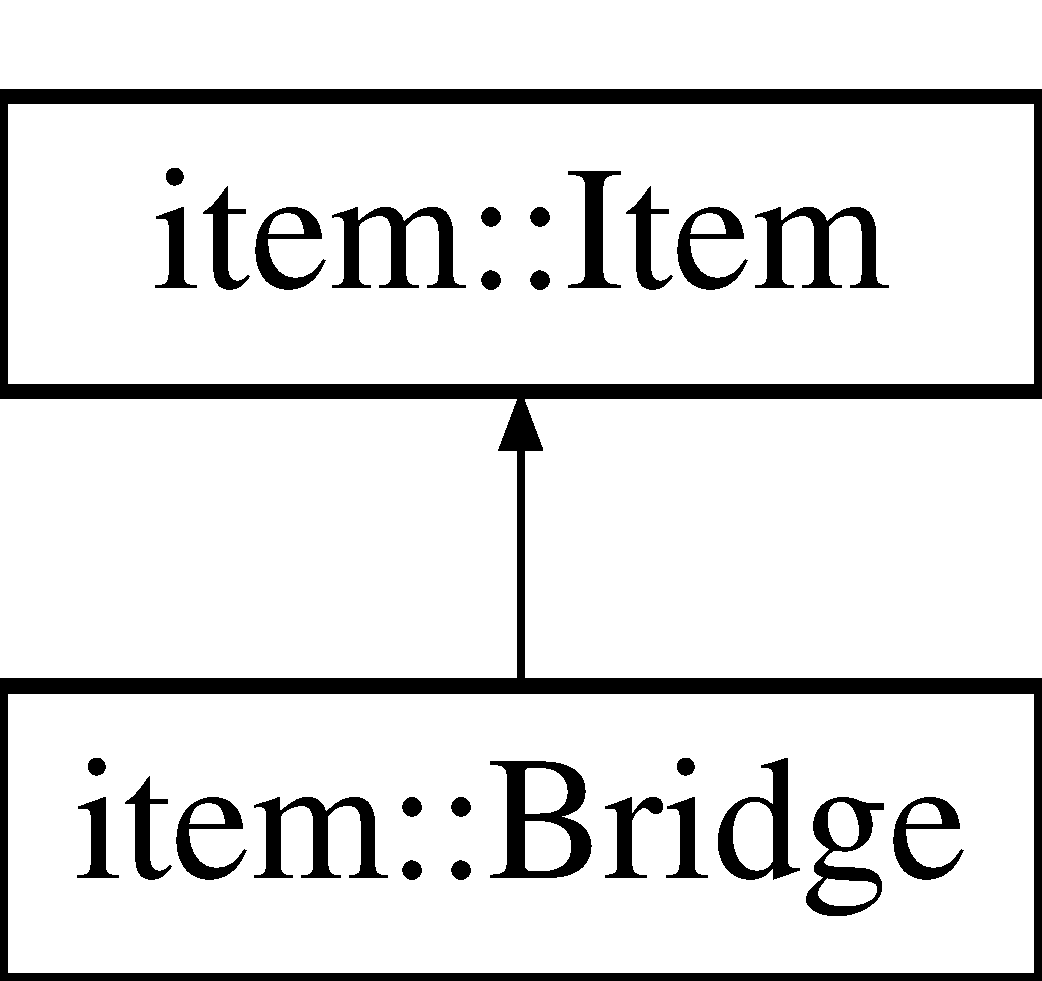
\includegraphics[height=2.000000cm]{classitem_1_1_bridge}
\end{center}
\end{figure}
\subsection*{Public Member Functions}
\begin{DoxyCompactItemize}
\item 
\mbox{\Hypertarget{classitem_1_1_bridge_a5bc97b39c3fcb52578942f5f41d7bb7d}\label{classitem_1_1_bridge_a5bc97b39c3fcb52578942f5f41d7bb7d}} 
{\bfseries Bridge} (\hyperlink{classtimeplane_1_1_moment}{Moment} first\+\_\+moment)
\item 
\hyperlink{classitem_1_1_effect}{Effect} \hyperlink{classitem_1_1_bridge_a7d579da1f368ba6a6b5dfd41de833f17}{View} (\hyperlink{classtimeplane_1_1_moment}{Moment} m)
\begin{DoxyCompactList}\small\item\em View the effects of an item at a specific moment. \end{DoxyCompactList}\item 
Tags \hyperlink{classitem_1_1_bridge_af49adc6bbaf4788cce2b4cbf8d895865}{State\+Tags} (\hyperlink{classtimeplane_1_1_moment}{Moment} m) const
\begin{DoxyCompactList}\small\item\em Virtual method to provide user-\/friendly tagged values. \end{DoxyCompactList}\end{DoxyCompactItemize}
\subsection*{Static Public Attributes}
\begin{DoxyCompactItemize}
\item 
static Item\+Type constexpr \hyperlink{classitem_1_1_bridge_aeb376b4b999ec6144454cd806e5e06d2}{type} = Item\+Type\+::k\+Bridge
\begin{DoxyCompactList}\small\item\em An enum representation of the type of the item. \end{DoxyCompactList}\item 
\mbox{\Hypertarget{classitem_1_1_bridge_ad779bb244833ce97048e1a105ff09a8f}\label{classitem_1_1_bridge_ad779bb244833ce97048e1a105ff09a8f}} 
static int constexpr \hyperlink{classitem_1_1_bridge_ad779bb244833ce97048e1a105ff09a8f}{k\+Unlock\+Requirement} = 45
\begin{DoxyCompactList}\small\item\em Energy requirement to unlock the item. \end{DoxyCompactList}\end{DoxyCompactItemize}
\subsection*{Protected Member Functions}
\begin{DoxyCompactItemize}
\item 
std\+::pair$<$ \hyperlink{classitem_1_1_effect}{Effect}, \hyperlink{classitem_1_1_item_properties}{Item\+Properties} $>$ \hyperlink{classitem_1_1_bridge_a08aa3fdb36e203e489bc0af65dde451c}{Step\+Impl} (\hyperlink{classtimeplane_1_1_moment}{Moment} curr, \hyperlink{classroundinfo_1_1_round_info_view}{Round\+Info\+View} const \&round\+\_\+info\+\_\+view, int energy\+\_\+input)
\begin{DoxyCompactList}\small\item\em Virtual method for computing the results of making a step. \end{DoxyCompactList}\item 
std\+::pair$<$ \hyperlink{classitem_1_1_effect}{Effect}, \hyperlink{classitem_1_1_item_properties}{Item\+Properties} $>$ \hyperlink{classitem_1_1_bridge_a175b2a911174c682ea163bc248836a87}{Branch\+Impl} (\hyperlink{classtimeplane_1_1_moment}{Moment} curr, \hyperlink{classtimeplane_1_1_moment}{Moment} dest)
\begin{DoxyCompactList}\small\item\em Virtual method for computing the results of branching. \end{DoxyCompactList}\end{DoxyCompactItemize}
\subsection*{Additional Inherited Members}


\subsection{Detailed Description}
\hyperlink{classitem_1_1_item}{Item} which bridges together separated moments. 

Moments that are otherwise separated because the latest antitelephone arrival lies in between can be connected with the \hyperlink{classitem_1_1_bridge}{Bridge}. Then it would be possible to travel from the later moment to the earlier moment. 

\subsection{Member Function Documentation}
\mbox{\Hypertarget{classitem_1_1_bridge_a7d579da1f368ba6a6b5dfd41de833f17}\label{classitem_1_1_bridge_a7d579da1f368ba6a6b5dfd41de833f17}} 
\index{item\+::\+Bridge@{item\+::\+Bridge}!View@{View}}
\index{View@{View}!item\+::\+Bridge@{item\+::\+Bridge}}
\subsubsection{\texorpdfstring{View()}{View()}}
{\footnotesize\ttfamily \hyperlink{classitem_1_1_effect}{Effect} Bridge\+::\+View (\begin{DoxyParamCaption}\item[{\hyperlink{classtimeplane_1_1_moment}{Moment}}]{m }\end{DoxyParamCaption})\hspace{0.3cm}{\ttfamily [virtual]}}



View the effects of an item at a specific moment. 


\begin{DoxyParams}{Parameters}
{\em m} & The moment to query. \\
\hline
\end{DoxyParams}
\begin{DoxyReturn}{Returns}
The effects granted by the item at the specified moment. 
\end{DoxyReturn}


Implements \hyperlink{classitem_1_1_item_a400dfeabc4056d36bfd348ff9c51cf7d}{item\+::\+Item}.

\mbox{\Hypertarget{classitem_1_1_bridge_af49adc6bbaf4788cce2b4cbf8d895865}\label{classitem_1_1_bridge_af49adc6bbaf4788cce2b4cbf8d895865}} 
\index{item\+::\+Bridge@{item\+::\+Bridge}!State\+Tags@{State\+Tags}}
\index{State\+Tags@{State\+Tags}!item\+::\+Bridge@{item\+::\+Bridge}}
\subsubsection{\texorpdfstring{State\+Tags()}{StateTags()}}
{\footnotesize\ttfamily Tags Bridge\+::\+State\+Tags (\begin{DoxyParamCaption}\item[{\hyperlink{classtimeplane_1_1_moment}{Moment}}]{m }\end{DoxyParamCaption}) const\hspace{0.3cm}{\ttfamily [virtual]}}



Virtual method to provide user-\/friendly tagged values. 

The tags are used as a user-\/friendly indication of the internal state of the item at a given moment without revealing implementation detail, and can also be used to attach specific meaning to the abstract lockdown and cooldown values associated with all items. 
\begin{DoxyParams}{Parameters}
{\em m} & The moment to query. \\
\hline
\end{DoxyParams}
\begin{DoxyReturn}{Returns}
A group of tagged values describing the state of an item. 
\end{DoxyReturn}


Implements \hyperlink{classitem_1_1_item_acc560ac68be4f5781cd90cddfd602942}{item\+::\+Item}.

\mbox{\Hypertarget{classitem_1_1_bridge_a08aa3fdb36e203e489bc0af65dde451c}\label{classitem_1_1_bridge_a08aa3fdb36e203e489bc0af65dde451c}} 
\index{item\+::\+Bridge@{item\+::\+Bridge}!Step\+Impl@{Step\+Impl}}
\index{Step\+Impl@{Step\+Impl}!item\+::\+Bridge@{item\+::\+Bridge}}
\subsubsection{\texorpdfstring{Step\+Impl()}{StepImpl()}}
{\footnotesize\ttfamily std\+::pair$<$ \hyperlink{classitem_1_1_effect}{Effect}, \hyperlink{classitem_1_1_item_properties}{Item\+Properties} $>$ Bridge\+::\+Step\+Impl (\begin{DoxyParamCaption}\item[{\hyperlink{classtimeplane_1_1_moment}{Moment}}]{curr,  }\item[{\hyperlink{classroundinfo_1_1_round_info_view}{Round\+Info\+View} const \&}]{turn\+\_\+data,  }\item[{int}]{energy\+\_\+input }\end{DoxyParamCaption})\hspace{0.3cm}{\ttfamily [protected]}, {\ttfamily [virtual]}}



Virtual method for computing the results of making a step. 


\begin{DoxyParams}{Parameters}
{\em curr} & The current moment before the step. \\
\hline
{\em turn\+\_\+data} & The information about the turn just played. \\
\hline
\end{DoxyParams}
\begin{DoxyReturn}{Returns}
The effects granted by the item for the next round, and the properties of the item for the next round. 
\end{DoxyReturn}


Implements \hyperlink{classitem_1_1_item_a90df61c8a2a20144eb1100af5fb2d464}{item\+::\+Item}.

\mbox{\Hypertarget{classitem_1_1_bridge_a175b2a911174c682ea163bc248836a87}\label{classitem_1_1_bridge_a175b2a911174c682ea163bc248836a87}} 
\index{item\+::\+Bridge@{item\+::\+Bridge}!Branch\+Impl@{Branch\+Impl}}
\index{Branch\+Impl@{Branch\+Impl}!item\+::\+Bridge@{item\+::\+Bridge}}
\subsubsection{\texorpdfstring{Branch\+Impl()}{BranchImpl()}}
{\footnotesize\ttfamily std\+::pair$<$ \hyperlink{classitem_1_1_effect}{Effect}, \hyperlink{classitem_1_1_item_properties}{Item\+Properties} $>$ Bridge\+::\+Branch\+Impl (\begin{DoxyParamCaption}\item[{\hyperlink{classtimeplane_1_1_moment}{Moment}}]{curr,  }\item[{\hyperlink{classtimeplane_1_1_moment}{Moment}}]{dest }\end{DoxyParamCaption})\hspace{0.3cm}{\ttfamily [protected]}, {\ttfamily [virtual]}}



Virtual method for computing the results of branching. 


\begin{DoxyParams}{Parameters}
{\em curr} & The current moment before branching. \\
\hline
{\em dest} & The destination moment to reach. \\
\hline
\end{DoxyParams}
\begin{DoxyReturn}{Returns}
The effects granted by the item for the next round, and the properties of the item for the next round. 
\end{DoxyReturn}


Implements \hyperlink{classitem_1_1_item_afef6bdd5c1c734c67122e4118e9e1930}{item\+::\+Item}.



\subsection{Member Data Documentation}
\mbox{\Hypertarget{classitem_1_1_bridge_aeb376b4b999ec6144454cd806e5e06d2}\label{classitem_1_1_bridge_aeb376b4b999ec6144454cd806e5e06d2}} 
\index{item\+::\+Bridge@{item\+::\+Bridge}!type@{type}}
\index{type@{type}!item\+::\+Bridge@{item\+::\+Bridge}}
\subsubsection{\texorpdfstring{type}{type}}
{\footnotesize\ttfamily Item\+Type constexpr item\+::\+Bridge\+::type = Item\+Type\+::k\+Bridge\hspace{0.3cm}{\ttfamily [static]}}



An enum representation of the type of the item. 

The value of the enum is a unique value for each item, and are consecutive starting at 0 across all items. 

The documentation for this class was generated from the following files\+:\begin{DoxyCompactItemize}
\item 
K\+:/\+Personal Projects/\+Antitelephone\+Q\+T/src/bridge.\+hpp\item 
K\+:/\+Personal Projects/\+Antitelephone\+Q\+T/src/bridge.\+cpp\end{DoxyCompactItemize}

\hypertarget{classitem_1_1_effect}{}\section{item\+:\+:Effect Class Reference}
\label{classitem_1_1_effect}\index{item\+::\+Effect@{item\+::\+Effect}}
\subsection*{Public Member Functions}
\begin{DoxyCompactItemize}
\item 
\hyperlink{classitem_1_1_effect_a4260fb6ad9c8d3f63ca934fd4410d142}{Effect} (int \hyperlink{classitem_1_1_effect_adf8addd1eb339afebbcc9c7278b81d7c}{attack\+\_\+increase}=0, int \hyperlink{classitem_1_1_effect_ad74a155925b8072030afabf3bb13ba4a}{max\+\_\+hitpoint\+\_\+increase}=0, int \hyperlink{classitem_1_1_effect_a9a6f54d0eab7dd13b2ef14e04f6ddb56}{shield\+\_\+amount}=0, bool \hyperlink{classitem_1_1_effect_abd1c6fcf2c430da628787c535cdeb527}{antitelephone\+\_\+departure}=false, bool \hyperlink{classitem_1_1_effect_acb90e76e736868dd5307e8b6fe7e2e0d}{antitelephone\+\_\+dest\+\_\+allowed}=false, bool \hyperlink{classitem_1_1_effect_a05de623b49c24c11fdb765c61c0367d0}{player\+\_\+make\+\_\+active}=false)
\begin{DoxyCompactList}\small\item\em Constructor. \end{DoxyCompactList}\item 
int \hyperlink{classitem_1_1_effect_adf8addd1eb339afebbcc9c7278b81d7c}{attack\+\_\+increase} () const noexcept
\begin{DoxyCompactList}\small\item\em Accessor for the attack increase quantity. \end{DoxyCompactList}\item 
void \hyperlink{classitem_1_1_effect_a0a98eb24f70970c00b95cfa0a40f6a6a}{set\+\_\+attack\+\_\+increase} (int \hyperlink{classitem_1_1_effect_adf8addd1eb339afebbcc9c7278b81d7c}{attack\+\_\+increase}) noexcept
\begin{DoxyCompactList}\small\item\em Mutator for the attack increase quantity. \end{DoxyCompactList}\item 
int \hyperlink{classitem_1_1_effect_ad74a155925b8072030afabf3bb13ba4a}{max\+\_\+hitpoint\+\_\+increase} () const noexcept
\begin{DoxyCompactList}\small\item\em Accessor for the increase in maximum hitpoints. \end{DoxyCompactList}\item 
void \hyperlink{classitem_1_1_effect_af2710ca17d043b8aeb3360fd991e3140}{set\+\_\+max\+\_\+hitpoint\+\_\+increase} (int \hyperlink{classitem_1_1_effect_ad74a155925b8072030afabf3bb13ba4a}{max\+\_\+hitpoint\+\_\+increase}) noexcept
\begin{DoxyCompactList}\small\item\em Mutator for the increase in maximum hitpoints. \end{DoxyCompactList}\item 
int \hyperlink{classitem_1_1_effect_a9a6f54d0eab7dd13b2ef14e04f6ddb56}{shield\+\_\+amount} () const noexcept
\begin{DoxyCompactList}\small\item\em Accessor for the shield absorption strength. \end{DoxyCompactList}\item 
void \hyperlink{classitem_1_1_effect_a1610df003ab26e8ce4aafc5a13543e86}{set\+\_\+shield\+\_\+amount} (int \hyperlink{classitem_1_1_effect_a9a6f54d0eab7dd13b2ef14e04f6ddb56}{shield\+\_\+amount}) noexcept
\begin{DoxyCompactList}\small\item\em Mutator for the shield absorption strength. \end{DoxyCompactList}\item 
bool \hyperlink{classitem_1_1_effect_abd1c6fcf2c430da628787c535cdeb527}{antitelephone\+\_\+departure} () const noexcept
\begin{DoxyCompactList}\small\item\em Accessor for an explicit antitelephone departure. \end{DoxyCompactList}\item 
void \hyperlink{classitem_1_1_effect_a209135cb3afb7f25dfd56c5b7c9e2ffd}{set\+\_\+antitelephone\+\_\+departure} (bool \hyperlink{classitem_1_1_effect_abd1c6fcf2c430da628787c535cdeb527}{antitelephone\+\_\+departure}) noexcept
\begin{DoxyCompactList}\small\item\em Mutator for an explicit antitelephone departure. \end{DoxyCompactList}\item 
bool \hyperlink{classitem_1_1_effect_acb90e76e736868dd5307e8b6fe7e2e0d}{antitelephone\+\_\+dest\+\_\+allowed} () const noexcept
\begin{DoxyCompactList}\small\item\em Accessor for the explicit allowance of antitelephone travel. \end{DoxyCompactList}\item 
void \hyperlink{classitem_1_1_effect_add9197b674f7ebd90c6a412d4a65e0e1}{set\+\_\+antitelephone\+\_\+dest\+\_\+allowed} (bool \hyperlink{classitem_1_1_effect_acb90e76e736868dd5307e8b6fe7e2e0d}{antitelephone\+\_\+dest\+\_\+allowed}) noexcept
\begin{DoxyCompactList}\small\item\em Mutator for the explicit allowance of antitelephone travel. \end{DoxyCompactList}\item 
bool \hyperlink{classitem_1_1_effect_a05de623b49c24c11fdb765c61c0367d0}{player\+\_\+make\+\_\+active} () const noexcept
\begin{DoxyCompactList}\small\item\em Accessor for directly making the player actively controllable. \end{DoxyCompactList}\item 
void \hyperlink{classitem_1_1_effect_aedb5619a40edeb90776d14691cdb80b1}{set\+\_\+player\+\_\+make\+\_\+active} (bool \hyperlink{classitem_1_1_effect_a05de623b49c24c11fdb765c61c0367d0}{player\+\_\+make\+\_\+active}) noexcept
\begin{DoxyCompactList}\small\item\em Mutator for directly making the player actively controllable. \end{DoxyCompactList}\item 
\hyperlink{classitem_1_1_effect}{Effect} \hyperlink{classitem_1_1_effect_a81c4b4c173683d278e1eae7e4ab8048a}{operator+} (\hyperlink{classitem_1_1_effect}{Effect} const \&rhs)
\begin{DoxyCompactList}\small\item\em Addition operator to combine effects. \end{DoxyCompactList}\item 
\hyperlink{classitem_1_1_effect}{Effect} \& \hyperlink{classitem_1_1_effect_af0d65e5a848289bfd28bfe980da51915}{operator+=} (\hyperlink{classitem_1_1_effect}{Effect} const \&rhs)
\begin{DoxyCompactList}\small\item\em Addition assignment operator. \end{DoxyCompactList}\item 
{\footnotesize template$<$typename Archive $>$ }\\void \hyperlink{classitem_1_1_effect_a3a78c050c37dd9204aa35c25a0f65282}{serialize} (Archive \&ar, unsigned int const version)
\begin{DoxyCompactList}\small\item\em Serialization function. \end{DoxyCompactList}\end{DoxyCompactItemize}


\subsection{Constructor \& Destructor Documentation}
\mbox{\Hypertarget{classitem_1_1_effect_a4260fb6ad9c8d3f63ca934fd4410d142}\label{classitem_1_1_effect_a4260fb6ad9c8d3f63ca934fd4410d142}} 
\index{item\+::\+Effect@{item\+::\+Effect}!Effect@{Effect}}
\index{Effect@{Effect}!item\+::\+Effect@{item\+::\+Effect}}
\subsubsection{\texorpdfstring{Effect()}{Effect()}}
{\footnotesize\ttfamily item\+::\+Effect\+::\+Effect (\begin{DoxyParamCaption}\item[{int}]{attack\+\_\+increase = {\ttfamily 0},  }\item[{int}]{max\+\_\+hitpoint\+\_\+increase = {\ttfamily 0},  }\item[{int}]{shield\+\_\+amount = {\ttfamily 0},  }\item[{bool}]{antitelephone\+\_\+departure = {\ttfamily false},  }\item[{bool}]{antitelephone\+\_\+dest\+\_\+allowed = {\ttfamily false},  }\item[{bool}]{player\+\_\+make\+\_\+active = {\ttfamily false} }\end{DoxyParamCaption})\hspace{0.3cm}{\ttfamily [inline]}}



Constructor. 


\begin{DoxyParams}{Parameters}
{\em attack\+\_\+increase} & Increase in damage output. \\
\hline
{\em shield\+\_\+amount} & Increase in shield absorption. \\
\hline
{\em antitelephone\+\_\+dest\+\_\+allowed} & Whether to explicitly allow antitelephone travel in spite of normal rules. \\
\hline
{\em player\+\_\+make\+\_\+active} & Whether to make the player actively controllable in spite of normal rules \\
\hline
\end{DoxyParams}


\subsection{Member Function Documentation}
\mbox{\Hypertarget{classitem_1_1_effect_adf8addd1eb339afebbcc9c7278b81d7c}\label{classitem_1_1_effect_adf8addd1eb339afebbcc9c7278b81d7c}} 
\index{item\+::\+Effect@{item\+::\+Effect}!attack\+\_\+increase@{attack\+\_\+increase}}
\index{attack\+\_\+increase@{attack\+\_\+increase}!item\+::\+Effect@{item\+::\+Effect}}
\subsubsection{\texorpdfstring{attack\+\_\+increase()}{attack\_increase()}}
{\footnotesize\ttfamily int item\+::\+Effect\+::attack\+\_\+increase (\begin{DoxyParamCaption}{ }\end{DoxyParamCaption}) const\hspace{0.3cm}{\ttfamily [inline]}, {\ttfamily [noexcept]}}



Accessor for the attack increase quantity. 

\begin{DoxyReturn}{Returns}
Attack increase, in extra damage per encounter. 
\end{DoxyReturn}
\mbox{\Hypertarget{classitem_1_1_effect_a0a98eb24f70970c00b95cfa0a40f6a6a}\label{classitem_1_1_effect_a0a98eb24f70970c00b95cfa0a40f6a6a}} 
\index{item\+::\+Effect@{item\+::\+Effect}!set\+\_\+attack\+\_\+increase@{set\+\_\+attack\+\_\+increase}}
\index{set\+\_\+attack\+\_\+increase@{set\+\_\+attack\+\_\+increase}!item\+::\+Effect@{item\+::\+Effect}}
\subsubsection{\texorpdfstring{set\+\_\+attack\+\_\+increase()}{set\_attack\_increase()}}
{\footnotesize\ttfamily void item\+::\+Effect\+::set\+\_\+attack\+\_\+increase (\begin{DoxyParamCaption}\item[{int}]{attack\+\_\+increase }\end{DoxyParamCaption})\hspace{0.3cm}{\ttfamily [inline]}, {\ttfamily [noexcept]}}



Mutator for the attack increase quantity. 


\begin{DoxyParams}{Parameters}
{\em attack\+\_\+increase} & Attack increase, in extra damage per encounter. \\
\hline
\end{DoxyParams}
\mbox{\Hypertarget{classitem_1_1_effect_ad74a155925b8072030afabf3bb13ba4a}\label{classitem_1_1_effect_ad74a155925b8072030afabf3bb13ba4a}} 
\index{item\+::\+Effect@{item\+::\+Effect}!max\+\_\+hitpoint\+\_\+increase@{max\+\_\+hitpoint\+\_\+increase}}
\index{max\+\_\+hitpoint\+\_\+increase@{max\+\_\+hitpoint\+\_\+increase}!item\+::\+Effect@{item\+::\+Effect}}
\subsubsection{\texorpdfstring{max\+\_\+hitpoint\+\_\+increase()}{max\_hitpoint\_increase()}}
{\footnotesize\ttfamily int item\+::\+Effect\+::max\+\_\+hitpoint\+\_\+increase (\begin{DoxyParamCaption}{ }\end{DoxyParamCaption}) const\hspace{0.3cm}{\ttfamily [inline]}, {\ttfamily [noexcept]}}



Accessor for the increase in maximum hitpoints. 

\begin{DoxyReturn}{Returns}
Increase in maximum hit points granted to the player. 
\end{DoxyReturn}
\mbox{\Hypertarget{classitem_1_1_effect_af2710ca17d043b8aeb3360fd991e3140}\label{classitem_1_1_effect_af2710ca17d043b8aeb3360fd991e3140}} 
\index{item\+::\+Effect@{item\+::\+Effect}!set\+\_\+max\+\_\+hitpoint\+\_\+increase@{set\+\_\+max\+\_\+hitpoint\+\_\+increase}}
\index{set\+\_\+max\+\_\+hitpoint\+\_\+increase@{set\+\_\+max\+\_\+hitpoint\+\_\+increase}!item\+::\+Effect@{item\+::\+Effect}}
\subsubsection{\texorpdfstring{set\+\_\+max\+\_\+hitpoint\+\_\+increase()}{set\_max\_hitpoint\_increase()}}
{\footnotesize\ttfamily void item\+::\+Effect\+::set\+\_\+max\+\_\+hitpoint\+\_\+increase (\begin{DoxyParamCaption}\item[{int}]{max\+\_\+hitpoint\+\_\+increase }\end{DoxyParamCaption})\hspace{0.3cm}{\ttfamily [inline]}, {\ttfamily [noexcept]}}



Mutator for the increase in maximum hitpoints. 


\begin{DoxyParams}{Parameters}
{\em max\+\_\+hitpoint\+\_\+increase} & Increase in maximum hit points granted to the player. \\
\hline
\end{DoxyParams}
\mbox{\Hypertarget{classitem_1_1_effect_a9a6f54d0eab7dd13b2ef14e04f6ddb56}\label{classitem_1_1_effect_a9a6f54d0eab7dd13b2ef14e04f6ddb56}} 
\index{item\+::\+Effect@{item\+::\+Effect}!shield\+\_\+amount@{shield\+\_\+amount}}
\index{shield\+\_\+amount@{shield\+\_\+amount}!item\+::\+Effect@{item\+::\+Effect}}
\subsubsection{\texorpdfstring{shield\+\_\+amount()}{shield\_amount()}}
{\footnotesize\ttfamily int item\+::\+Effect\+::shield\+\_\+amount (\begin{DoxyParamCaption}{ }\end{DoxyParamCaption}) const\hspace{0.3cm}{\ttfamily [inline]}, {\ttfamily [noexcept]}}



Accessor for the shield absorption strength. 

\begin{DoxyReturn}{Returns}
\hyperlink{classitem_1_1_shield}{Shield} absorption, in damage absorbed by the shield. 
\end{DoxyReturn}
\mbox{\Hypertarget{classitem_1_1_effect_a1610df003ab26e8ce4aafc5a13543e86}\label{classitem_1_1_effect_a1610df003ab26e8ce4aafc5a13543e86}} 
\index{item\+::\+Effect@{item\+::\+Effect}!set\+\_\+shield\+\_\+amount@{set\+\_\+shield\+\_\+amount}}
\index{set\+\_\+shield\+\_\+amount@{set\+\_\+shield\+\_\+amount}!item\+::\+Effect@{item\+::\+Effect}}
\subsubsection{\texorpdfstring{set\+\_\+shield\+\_\+amount()}{set\_shield\_amount()}}
{\footnotesize\ttfamily void item\+::\+Effect\+::set\+\_\+shield\+\_\+amount (\begin{DoxyParamCaption}\item[{int}]{shield\+\_\+amount }\end{DoxyParamCaption})\hspace{0.3cm}{\ttfamily [inline]}, {\ttfamily [noexcept]}}



Mutator for the shield absorption strength. 


\begin{DoxyParams}{Parameters}
{\em shield\+\_\+amount} & \hyperlink{classitem_1_1_shield}{Shield} absorption, in damage absorbed by the shield. \\
\hline
\end{DoxyParams}
\mbox{\Hypertarget{classitem_1_1_effect_abd1c6fcf2c430da628787c535cdeb527}\label{classitem_1_1_effect_abd1c6fcf2c430da628787c535cdeb527}} 
\index{item\+::\+Effect@{item\+::\+Effect}!antitelephone\+\_\+departure@{antitelephone\+\_\+departure}}
\index{antitelephone\+\_\+departure@{antitelephone\+\_\+departure}!item\+::\+Effect@{item\+::\+Effect}}
\subsubsection{\texorpdfstring{antitelephone\+\_\+departure()}{antitelephone\_departure()}}
{\footnotesize\ttfamily bool item\+::\+Effect\+::antitelephone\+\_\+departure (\begin{DoxyParamCaption}{ }\end{DoxyParamCaption}) const\hspace{0.3cm}{\ttfamily [inline]}, {\ttfamily [noexcept]}}



Accessor for an explicit antitelephone departure. 

In general, a {\ttfamily true} value overrides any {\ttfamily false} values, so a value of {\ttfamily false} does not explicitly rule out antitelephone departure. \begin{DoxyReturn}{Returns}
Whether antitelephone departure has explicitly occurred. 
\end{DoxyReturn}
\mbox{\Hypertarget{classitem_1_1_effect_a209135cb3afb7f25dfd56c5b7c9e2ffd}\label{classitem_1_1_effect_a209135cb3afb7f25dfd56c5b7c9e2ffd}} 
\index{item\+::\+Effect@{item\+::\+Effect}!set\+\_\+antitelephone\+\_\+departure@{set\+\_\+antitelephone\+\_\+departure}}
\index{set\+\_\+antitelephone\+\_\+departure@{set\+\_\+antitelephone\+\_\+departure}!item\+::\+Effect@{item\+::\+Effect}}
\subsubsection{\texorpdfstring{set\+\_\+antitelephone\+\_\+departure()}{set\_antitelephone\_departure()}}
{\footnotesize\ttfamily void item\+::\+Effect\+::set\+\_\+antitelephone\+\_\+departure (\begin{DoxyParamCaption}\item[{bool}]{antitelephone\+\_\+departure }\end{DoxyParamCaption})\hspace{0.3cm}{\ttfamily [inline]}, {\ttfamily [noexcept]}}



Mutator for an explicit antitelephone departure. 


\begin{DoxyParams}{Parameters}
{\em antitelephone\+\_\+departure} & Whether antitelephone departure has explicitly occurred. \\
\hline
\end{DoxyParams}
\mbox{\Hypertarget{classitem_1_1_effect_acb90e76e736868dd5307e8b6fe7e2e0d}\label{classitem_1_1_effect_acb90e76e736868dd5307e8b6fe7e2e0d}} 
\index{item\+::\+Effect@{item\+::\+Effect}!antitelephone\+\_\+dest\+\_\+allowed@{antitelephone\+\_\+dest\+\_\+allowed}}
\index{antitelephone\+\_\+dest\+\_\+allowed@{antitelephone\+\_\+dest\+\_\+allowed}!item\+::\+Effect@{item\+::\+Effect}}
\subsubsection{\texorpdfstring{antitelephone\+\_\+dest\+\_\+allowed()}{antitelephone\_dest\_allowed()}}
{\footnotesize\ttfamily bool item\+::\+Effect\+::antitelephone\+\_\+dest\+\_\+allowed (\begin{DoxyParamCaption}{ }\end{DoxyParamCaption}) const\hspace{0.3cm}{\ttfamily [inline]}, {\ttfamily [noexcept]}}



Accessor for the explicit allowance of antitelephone travel. 

In general, a {\ttfamily true} value overrides any {\ttfamily false} values, so a value of {\ttfamily false} does not explicitly disallow antitelephone travel. \begin{DoxyReturn}{Returns}
Whether antitelephone travel is explicitly allowed. 
\end{DoxyReturn}
\mbox{\Hypertarget{classitem_1_1_effect_add9197b674f7ebd90c6a412d4a65e0e1}\label{classitem_1_1_effect_add9197b674f7ebd90c6a412d4a65e0e1}} 
\index{item\+::\+Effect@{item\+::\+Effect}!set\+\_\+antitelephone\+\_\+dest\+\_\+allowed@{set\+\_\+antitelephone\+\_\+dest\+\_\+allowed}}
\index{set\+\_\+antitelephone\+\_\+dest\+\_\+allowed@{set\+\_\+antitelephone\+\_\+dest\+\_\+allowed}!item\+::\+Effect@{item\+::\+Effect}}
\subsubsection{\texorpdfstring{set\+\_\+antitelephone\+\_\+dest\+\_\+allowed()}{set\_antitelephone\_dest\_allowed()}}
{\footnotesize\ttfamily void item\+::\+Effect\+::set\+\_\+antitelephone\+\_\+dest\+\_\+allowed (\begin{DoxyParamCaption}\item[{bool}]{antitelephone\+\_\+dest\+\_\+allowed }\end{DoxyParamCaption})\hspace{0.3cm}{\ttfamily [inline]}, {\ttfamily [noexcept]}}



Mutator for the explicit allowance of antitelephone travel. 


\begin{DoxyParams}{Parameters}
{\em antitelephone\+\_\+dest\+\_\+allowed} & Whether antitelephone travel is explicitly allowed. \\
\hline
\end{DoxyParams}
\mbox{\Hypertarget{classitem_1_1_effect_a05de623b49c24c11fdb765c61c0367d0}\label{classitem_1_1_effect_a05de623b49c24c11fdb765c61c0367d0}} 
\index{item\+::\+Effect@{item\+::\+Effect}!player\+\_\+make\+\_\+active@{player\+\_\+make\+\_\+active}}
\index{player\+\_\+make\+\_\+active@{player\+\_\+make\+\_\+active}!item\+::\+Effect@{item\+::\+Effect}}
\subsubsection{\texorpdfstring{player\+\_\+make\+\_\+active()}{player\_make\_active()}}
{\footnotesize\ttfamily bool item\+::\+Effect\+::player\+\_\+make\+\_\+active (\begin{DoxyParamCaption}{ }\end{DoxyParamCaption}) const\hspace{0.3cm}{\ttfamily [inline]}, {\ttfamily [noexcept]}}



Accessor for directly making the player actively controllable. 

In general, a {\ttfamily true} value overrides any {\ttfamily false} values, so a value of {\ttfamily false} does not force the player to be uncontrollable. \begin{DoxyReturn}{Returns}
Whether the player is directly to be made controllable. 
\end{DoxyReturn}
\mbox{\Hypertarget{classitem_1_1_effect_aedb5619a40edeb90776d14691cdb80b1}\label{classitem_1_1_effect_aedb5619a40edeb90776d14691cdb80b1}} 
\index{item\+::\+Effect@{item\+::\+Effect}!set\+\_\+player\+\_\+make\+\_\+active@{set\+\_\+player\+\_\+make\+\_\+active}}
\index{set\+\_\+player\+\_\+make\+\_\+active@{set\+\_\+player\+\_\+make\+\_\+active}!item\+::\+Effect@{item\+::\+Effect}}
\subsubsection{\texorpdfstring{set\+\_\+player\+\_\+make\+\_\+active()}{set\_player\_make\_active()}}
{\footnotesize\ttfamily void item\+::\+Effect\+::set\+\_\+player\+\_\+make\+\_\+active (\begin{DoxyParamCaption}\item[{bool}]{player\+\_\+make\+\_\+active }\end{DoxyParamCaption})\hspace{0.3cm}{\ttfamily [inline]}, {\ttfamily [noexcept]}}



Mutator for directly making the player actively controllable. 


\begin{DoxyParams}{Parameters}
{\em player\+\_\+make\+\_\+active} & Whether the player is directly to be made controllable. \\
\hline
\end{DoxyParams}
\mbox{\Hypertarget{classitem_1_1_effect_a81c4b4c173683d278e1eae7e4ab8048a}\label{classitem_1_1_effect_a81c4b4c173683d278e1eae7e4ab8048a}} 
\index{item\+::\+Effect@{item\+::\+Effect}!operator+@{operator+}}
\index{operator+@{operator+}!item\+::\+Effect@{item\+::\+Effect}}
\subsubsection{\texorpdfstring{operator+()}{operator+()}}
{\footnotesize\ttfamily \hyperlink{classitem_1_1_effect}{Effect} item\+::\+Effect\+::operator+ (\begin{DoxyParamCaption}\item[{\hyperlink{classitem_1_1_effect}{Effect} const \&}]{rhs }\end{DoxyParamCaption})\hspace{0.3cm}{\ttfamily [inline]}}



Addition operator to combine effects. 

The attack increase and shield absorption strength is added directly. The boolean values are combined with a boolean OR operation. 
\begin{DoxyParams}{Parameters}
{\em rhs} & The other {\ttfamily \hyperlink{classitem_1_1_effect}{Effect}} to combine with. \\
\hline
\end{DoxyParams}
\begin{DoxyReturn}{Returns}
The combined effect of the two inputs. 
\end{DoxyReturn}
\mbox{\Hypertarget{classitem_1_1_effect_af0d65e5a848289bfd28bfe980da51915}\label{classitem_1_1_effect_af0d65e5a848289bfd28bfe980da51915}} 
\index{item\+::\+Effect@{item\+::\+Effect}!operator+=@{operator+=}}
\index{operator+=@{operator+=}!item\+::\+Effect@{item\+::\+Effect}}
\subsubsection{\texorpdfstring{operator+=()}{operator+=()}}
{\footnotesize\ttfamily \hyperlink{classitem_1_1_effect}{Effect}\& item\+::\+Effect\+::operator+= (\begin{DoxyParamCaption}\item[{\hyperlink{classitem_1_1_effect}{Effect} const \&}]{rhs }\end{DoxyParamCaption})\hspace{0.3cm}{\ttfamily [inline]}}



Addition assignment operator. 

\begin{DoxySeeAlso}{See also}
operator+ 
\end{DoxySeeAlso}

\begin{DoxyParams}{Parameters}
{\em rhs} & The other {\ttfamily \hyperlink{classitem_1_1_effect}{Effect}} to combine with. \\
\hline
\end{DoxyParams}
\begin{DoxyReturn}{Returns}
The left hand side, after modification. 
\end{DoxyReturn}
\mbox{\Hypertarget{classitem_1_1_effect_a3a78c050c37dd9204aa35c25a0f65282}\label{classitem_1_1_effect_a3a78c050c37dd9204aa35c25a0f65282}} 
\index{item\+::\+Effect@{item\+::\+Effect}!serialize@{serialize}}
\index{serialize@{serialize}!item\+::\+Effect@{item\+::\+Effect}}
\subsubsection{\texorpdfstring{serialize()}{serialize()}}
{\footnotesize\ttfamily template$<$typename Archive $>$ \\
void item\+::\+Effect\+::serialize (\begin{DoxyParamCaption}\item[{Archive \&}]{ar,  }\item[{unsigned int const}]{version }\end{DoxyParamCaption})\hspace{0.3cm}{\ttfamily [inline]}}



Serialization function. 


\begin{DoxyTemplParams}{Template Parameters}
{\em Archive} & The serialization archive type. \\
\hline
\end{DoxyTemplParams}

\begin{DoxyParams}{Parameters}
{\em ar} & The serialization archive. \\
\hline
{\em version} & The verion of the serialization protocol to use. \\
\hline
\end{DoxyParams}


The documentation for this class was generated from the following file\+:\begin{DoxyCompactItemize}
\item 
K\+:/\+Personal Projects/\+Antitelephone\+Q\+T/src/effect.\+hpp\end{DoxyCompactItemize}

\hypertarget{structstd_1_1hash_3_01timeplane_1_1_moment_01_4}{}\section{std\+:\+:hash$<$ timeplane\+:\+:Moment $>$ Struct Template Reference}
\label{structstd_1_1hash_3_01timeplane_1_1_moment_01_4}\index{std\+::hash$<$ timeplane\+::\+Moment $>$@{std\+::hash$<$ timeplane\+::\+Moment $>$}}


Hash function for {\ttfamily Moment} instances.  




{\ttfamily \#include $<$moment.\+hpp$>$}

\subsection*{Public Member Functions}
\begin{DoxyCompactItemize}
\item 
\mbox{\Hypertarget{structstd_1_1hash_3_01timeplane_1_1_moment_01_4_ad80181ebc12d459ea83dd1f62ddb6713}\label{structstd_1_1hash_3_01timeplane_1_1_moment_01_4_ad80181ebc12d459ea83dd1f62ddb6713}} 
size\+\_\+t {\bfseries operator()} (const \hyperlink{classtimeplane_1_1_moment}{timeplane\+::\+Moment} \&m) const
\end{DoxyCompactItemize}


\subsection{Detailed Description}
\subsubsection*{template$<$$>$\newline
struct std\+::hash$<$ timeplane\+::\+Moment $>$}

Hash function for {\ttfamily Moment} instances. 

The documentation for this struct was generated from the following file\+:\begin{DoxyCompactItemize}
\item 
K\+:/\+Personal Projects/\+Antitelephone\+Q\+T/src/moment.\+hpp\end{DoxyCompactItemize}

\hypertarget{classitem_1_1_item}{}\section{item\+:\+:Item Class Reference}
\label{classitem_1_1_item}\index{item\+::\+Item@{item\+::\+Item}}


The properties of an item in the game across moments.  




{\ttfamily \#include $<$item.\+hpp$>$}

Inheritance diagram for item\+:\+:Item\+:\begin{figure}[H]
\begin{center}
\leavevmode
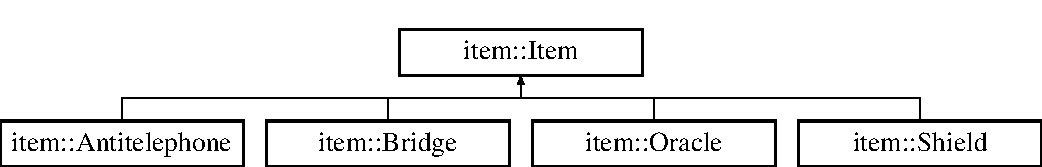
\includegraphics[height=2.000000cm]{classitem_1_1_item}
\end{center}
\end{figure}
\subsection*{Public Member Functions}
\begin{DoxyCompactItemize}
\item 
\hyperlink{classitem_1_1_effect}{Effect} \hyperlink{classitem_1_1_item_ad8d77979820782fd86a0a67e2ea25c75}{Step} (\hyperlink{classtimeplane_1_1_moment}{Moment} curr, \hyperlink{classroundinfo_1_1_round_info_view}{Round\+Info\+View} const \&round\+\_\+info\+\_\+view, int energy\+\_\+input)
\begin{DoxyCompactList}\small\item\em Update the item across a regular step into the future. \end{DoxyCompactList}\item 
\hyperlink{classitem_1_1_effect}{Effect} \hyperlink{classitem_1_1_item_aa4b1c982b6d35d047c7a8ea86b06be99}{Branch} (\hyperlink{classtimeplane_1_1_moment}{Moment} curr, \hyperlink{classtimeplane_1_1_moment}{Moment} dest)
\begin{DoxyCompactList}\small\item\em Update the item while traveling to the past (branching). \end{DoxyCompactList}\item 
void \hyperlink{classitem_1_1_item_a99eaccdd31a817a7cb0e501cb632f711}{Confirm\+Pending} (\hyperlink{classtimeplane_1_1_moment}{Moment} new\+\_\+moment)
\begin{DoxyCompactList}\small\item\em Finalize the changes in the item. \end{DoxyCompactList}\item 
virtual \hyperlink{classitem_1_1_effect}{Effect} \hyperlink{classitem_1_1_item_a7d2b010a27fec55e04a56e7c4fca7837}{View} (\hyperlink{classtimeplane_1_1_moment}{Moment} m) const =0
\begin{DoxyCompactList}\small\item\em View the effects of an item at a specific moment. \end{DoxyCompactList}\item 
void \hyperlink{classitem_1_1_item_ab31c1b5e2b0993341e7a268693960b90}{Duplicate} (\hyperlink{classtimeplane_1_1_moment}{Moment} to\+\_\+duplicate)
\begin{DoxyCompactList}\small\item\em Duplicates the item properties at the specified moment. \end{DoxyCompactList}\item 
virtual Tagged\+Values \hyperlink{classitem_1_1_item_a8410ab3ab75e65360eddb4f6bd3cceff}{State\+Tagged\+Values} (\hyperlink{classtimeplane_1_1_moment}{Moment} m) const =0
\begin{DoxyCompactList}\small\item\em Virtual method to provide user-\/friendly tagged values. \end{DoxyCompactList}\item 
void \hyperlink{classitem_1_1_item_a8d78594540bff88538723a8a1fb881d5}{Moment\+Deleter} (timeplane\+::\+Moment\+Iterators iterators)
\begin{DoxyCompactList}\small\item\em Function to clean up data related to inaccessible moments. \end{DoxyCompactList}\end{DoxyCompactItemize}
\subsection*{Static Public Attributes}
\begin{DoxyCompactItemize}
\item 
\mbox{\Hypertarget{classitem_1_1_item_aae2db5aecbcd2703453521c457bc9419}\label{classitem_1_1_item_aae2db5aecbcd2703453521c457bc9419}} 
static int constexpr \hyperlink{classitem_1_1_item_aae2db5aecbcd2703453521c457bc9419}{k\+Max\+Cooldown} = 4
\begin{DoxyCompactList}\small\item\em Maximum cooldown of items, by default. \end{DoxyCompactList}\item 
\mbox{\Hypertarget{classitem_1_1_item_a445a6061775c6a8cd3ce4e984698b9f6}\label{classitem_1_1_item_a445a6061775c6a8cd3ce4e984698b9f6}} 
static int constexpr \hyperlink{classitem_1_1_item_a445a6061775c6a8cd3ce4e984698b9f6}{k\+Basic\+Max\+Hitpoints} = 20
\begin{DoxyCompactList}\small\item\em Maximum hitpoints the player has as a basic guarantee. \end{DoxyCompactList}\item 
\mbox{\Hypertarget{classitem_1_1_item_a30b4c60171ecd398d5ff79f5340f40cb}\label{classitem_1_1_item_a30b4c60171ecd398d5ff79f5340f40cb}} 
static int constexpr \hyperlink{classitem_1_1_item_a30b4c60171ecd398d5ff79f5340f40cb}{k\+Max\+Hitpoint\+Increment} = 20
\begin{DoxyCompactList}\small\item\em Maximum hitpoints gained for each new unlocked item. \end{DoxyCompactList}\item 
\mbox{\Hypertarget{classitem_1_1_item_a198b43663d2cafe26b5a495738882df7}\label{classitem_1_1_item_a198b43663d2cafe26b5a495738882df7}} 
static int constexpr \hyperlink{classitem_1_1_item_a198b43663d2cafe26b5a495738882df7}{k\+Basic\+Attack} = 4
\begin{DoxyCompactList}\small\item\em Maximum hitpoints the player has as a basic guarantee. \end{DoxyCompactList}\item 
\mbox{\Hypertarget{classitem_1_1_item_a00def77d22585b09011b09981f3ad3b6}\label{classitem_1_1_item_a00def77d22585b09011b09981f3ad3b6}} 
static int constexpr \hyperlink{classitem_1_1_item_a00def77d22585b09011b09981f3ad3b6}{k\+Attack\+Increment} = 4
\begin{DoxyCompactList}\small\item\em Attack boost gained for each new unlocked item. \end{DoxyCompactList}\end{DoxyCompactItemize}
\subsection*{Protected Member Functions}
\begin{DoxyCompactItemize}
\item 
\hyperlink{classitem_1_1_item_aebe9569e9074ee805b6213f500066115}{Item} (\hyperlink{classtimeplane_1_1_moment}{Moment} first\+\_\+moment, \hyperlink{classitem_1_1_item_properties}{Item\+Properties} const \&first\+\_\+properties)
\begin{DoxyCompactList}\small\item\em Constructor. \end{DoxyCompactList}\item 
\hyperlink{classitem_1_1_item_properties}{Item\+Properties} const  \& \hyperlink{classitem_1_1_item_a23790dceafc9e3f8950f69380cc4c4aa}{Get\+Properties} (\hyperlink{classtimeplane_1_1_moment}{Moment} m) const
\begin{DoxyCompactList}\small\item\em Accessor for the properties of an item at a specific moment. \end{DoxyCompactList}\item 
\hyperlink{classitem_1_1_effect}{Effect} \hyperlink{classitem_1_1_item_a35583f2bcdaea50728a9e16e0626e341}{Increment\+Effect\+If} (\hyperlink{classtimeplane_1_1_moment}{Moment} m) const
\begin{DoxyCompactList}\small\item\em {\ttfamily \hyperlink{classitem_1_1_effect}{Effect}} instance with an attack and maximum hitpoint increase. \end{DoxyCompactList}\item 
virtual std\+::pair$<$ \hyperlink{classitem_1_1_effect}{Effect}, \hyperlink{classitem_1_1_item_properties}{Item\+Properties} $>$ \hyperlink{classitem_1_1_item_a90df61c8a2a20144eb1100af5fb2d464}{Step\+Impl} (\hyperlink{classtimeplane_1_1_moment}{Moment} curr, \hyperlink{classroundinfo_1_1_round_info_view}{Round\+Info\+View} const \&turn\+\_\+data, int energy\+\_\+input)=0
\begin{DoxyCompactList}\small\item\em Virtual method for computing the results of making a step. \end{DoxyCompactList}\item 
virtual std\+::pair$<$ \hyperlink{classitem_1_1_effect}{Effect}, \hyperlink{classitem_1_1_item_properties}{Item\+Properties} $>$ \hyperlink{classitem_1_1_item_afef6bdd5c1c734c67122e4118e9e1930}{Branch\+Impl} (\hyperlink{classtimeplane_1_1_moment}{Moment} curr, \hyperlink{classtimeplane_1_1_moment}{Moment} dest)=0
\begin{DoxyCompactList}\small\item\em Virtual method for computing the results of branching. \end{DoxyCompactList}\end{DoxyCompactItemize}
\subsection*{Static Protected Member Functions}
\begin{DoxyCompactItemize}
\item 
static \hyperlink{classitem_1_1_effect}{Effect} \hyperlink{classitem_1_1_item_a69a02566ccfd21e054e48864a9d4362e}{Basic\+Effect} () noexcept
\begin{DoxyCompactList}\small\item\em {\ttfamily \hyperlink{classitem_1_1_effect}{Effect}} instance with basic attack and maximum hitpoints. \end{DoxyCompactList}\item 
static \hyperlink{classitem_1_1_effect}{Effect} \hyperlink{classitem_1_1_item_abaff3ea78fa8c9940868b99ce8b6d2ea}{Increment\+Effect\+If} (\hyperlink{classitem_1_1_item_properties}{Item\+Properties} const \&p) noexcept
\begin{DoxyCompactList}\small\item\em {\ttfamily \hyperlink{classitem_1_1_effect}{Effect}} instance with an attack and maximum hitpoint increase. \end{DoxyCompactList}\item 
static bool \hyperlink{classitem_1_1_item_a93ef8f291ecf2886ea6902d496624334}{Standard\+Step\+Update} (\hyperlink{classitem_1_1_item_properties}{Item\+Properties} \&properties, int energy\+\_\+input)
\begin{DoxyCompactList}\small\item\em Standard update algorithm for properties. \end{DoxyCompactList}\end{DoxyCompactItemize}


\subsection{Detailed Description}
The properties of an item in the game across moments. 

This class contains is virtual and cannot be instantiated directly. The various items in the game inherit from this type.

Information about an item is always future-\/oriented, which means the effects and state tags describing an item at a specific moment apply to the moment as it occurs, instead of being a result of said moment after it has already passed. 

\subsection{Constructor \& Destructor Documentation}
\mbox{\Hypertarget{classitem_1_1_item_aebe9569e9074ee805b6213f500066115}\label{classitem_1_1_item_aebe9569e9074ee805b6213f500066115}} 
\index{item\+::\+Item@{item\+::\+Item}!Item@{Item}}
\index{Item@{Item}!item\+::\+Item@{item\+::\+Item}}
\subsubsection{\texorpdfstring{Item()}{Item()}}
{\footnotesize\ttfamily Item\+::\+Item (\begin{DoxyParamCaption}\item[{\hyperlink{classtimeplane_1_1_moment}{Moment}}]{first\+\_\+moment,  }\item[{\hyperlink{classitem_1_1_item_properties}{Item\+Properties} const \&}]{first\+\_\+properties }\end{DoxyParamCaption})\hspace{0.3cm}{\ttfamily [protected]}}



Constructor. 


\begin{DoxyParams}{Parameters}
{\em first\+\_\+moment} & The first moment in the game. \\
\hline
\end{DoxyParams}


\subsection{Member Function Documentation}
\mbox{\Hypertarget{classitem_1_1_item_ad8d77979820782fd86a0a67e2ea25c75}\label{classitem_1_1_item_ad8d77979820782fd86a0a67e2ea25c75}} 
\index{item\+::\+Item@{item\+::\+Item}!Step@{Step}}
\index{Step@{Step}!item\+::\+Item@{item\+::\+Item}}
\subsubsection{\texorpdfstring{Step()}{Step()}}
{\footnotesize\ttfamily \hyperlink{classitem_1_1_effect}{Effect} Item\+::\+Step (\begin{DoxyParamCaption}\item[{\hyperlink{classtimeplane_1_1_moment}{Moment}}]{curr,  }\item[{\hyperlink{classroundinfo_1_1_round_info_view}{Round\+Info\+View} const \&}]{round\+\_\+info\+\_\+view,  }\item[{int}]{energy\+\_\+input }\end{DoxyParamCaption})}



Update the item across a regular step into the future. 

The resulting item properties are stored temporarily until the client calls {\ttfamily Confirm\+Pending} to finalize them. The item properties are updated after considering the events that have occurred in the turn. The round information parameter is in a past-\/oriented state, so all future-\/oriented values in the instance is unspecified. 
\begin{DoxyParams}{Parameters}
{\em curr} & The current moment before the step. \\
\hline
{\em round\+\_\+info} & The information about the turn just played. \\
\hline
\end{DoxyParams}
\begin{DoxyReturn}{Returns}
The effects granted by the item for the next round. 
\end{DoxyReturn}

\begin{DoxyExceptions}{Exceptions}
{\em std\+::out\+\_\+of\+\_\+range} & Potentially thrown by subclasses. \\
\hline
\end{DoxyExceptions}
\mbox{\Hypertarget{classitem_1_1_item_aa4b1c982b6d35d047c7a8ea86b06be99}\label{classitem_1_1_item_aa4b1c982b6d35d047c7a8ea86b06be99}} 
\index{item\+::\+Item@{item\+::\+Item}!Branch@{Branch}}
\index{Branch@{Branch}!item\+::\+Item@{item\+::\+Item}}
\subsubsection{\texorpdfstring{Branch()}{Branch()}}
{\footnotesize\ttfamily \hyperlink{classitem_1_1_effect}{Effect} Item\+::\+Branch (\begin{DoxyParamCaption}\item[{\hyperlink{classtimeplane_1_1_moment}{Moment}}]{curr,  }\item[{\hyperlink{classtimeplane_1_1_moment}{Moment}}]{dest }\end{DoxyParamCaption})}



Update the item while traveling to the past (branching). 

The resulting item properties are stored temporarily until the client calls {\ttfamily Confirm\+Pending} to finalize them. 
\begin{DoxyParams}{Parameters}
{\em curr} & The current moment before branching. \\
\hline
{\em dest} & The destination moment to reach. \\
\hline
\end{DoxyParams}
\begin{DoxyReturn}{Returns}
The effects granted by the item for the next round. 
\end{DoxyReturn}

\begin{DoxyExceptions}{Exceptions}
{\em std\+::invalid\+\_\+argument} & If the destination is not in the past. \\
\hline
{\em std\+::out\+\_\+of\+\_\+range} & Potentially thrown by subclasses. \\
\hline
\end{DoxyExceptions}
\mbox{\Hypertarget{classitem_1_1_item_a99eaccdd31a817a7cb0e501cb632f711}\label{classitem_1_1_item_a99eaccdd31a817a7cb0e501cb632f711}} 
\index{item\+::\+Item@{item\+::\+Item}!Confirm\+Pending@{Confirm\+Pending}}
\index{Confirm\+Pending@{Confirm\+Pending}!item\+::\+Item@{item\+::\+Item}}
\subsubsection{\texorpdfstring{Confirm\+Pending()}{ConfirmPending()}}
{\footnotesize\ttfamily void Item\+::\+Confirm\+Pending (\begin{DoxyParamCaption}\item[{\hyperlink{classtimeplane_1_1_moment}{Moment}}]{new\+\_\+moment }\end{DoxyParamCaption})}



Finalize the changes in the item. 

This requires that the new moment occurs at time one more than the one provided to {\ttfamily Step}, or has the same time as the destination moment providede to {\ttfamily Branch}. 
\begin{DoxyParams}{Parameters}
{\em new\+\_\+moment} & The moment to associate with item changes. \\
\hline
\end{DoxyParams}
\mbox{\Hypertarget{classitem_1_1_item_a7d2b010a27fec55e04a56e7c4fca7837}\label{classitem_1_1_item_a7d2b010a27fec55e04a56e7c4fca7837}} 
\index{item\+::\+Item@{item\+::\+Item}!View@{View}}
\index{View@{View}!item\+::\+Item@{item\+::\+Item}}
\subsubsection{\texorpdfstring{View()}{View()}}
{\footnotesize\ttfamily virtual \hyperlink{classitem_1_1_effect}{Effect} item\+::\+Item\+::\+View (\begin{DoxyParamCaption}\item[{\hyperlink{classtimeplane_1_1_moment}{Moment}}]{m }\end{DoxyParamCaption}) const\hspace{0.3cm}{\ttfamily [pure virtual]}}



View the effects of an item at a specific moment. 

This call must be a pure function not only of the provided moment, but also be a function of {\ttfamily Get\+Properties(m)}. 
\begin{DoxyParams}{Parameters}
{\em m} & The moment to query. \\
\hline
\end{DoxyParams}
\begin{DoxyReturn}{Returns}
The effects granted by the item at the specified moment. 
\end{DoxyReturn}

\begin{DoxyExceptions}{Exceptions}
{\em std\+::out\+\_\+of\+\_\+range} & Potentially thrown by subclasses. \\
\hline
\end{DoxyExceptions}


Implemented in \hyperlink{classitem_1_1_bridge_a644ccbcba577629cd0f07066e64afac1}{item\+::\+Bridge}, \hyperlink{classitem_1_1_oracle_ade8c5db0ab73bfa61d5dbe2c9c405f5c}{item\+::\+Oracle}, \hyperlink{classitem_1_1_shield_ae4a97ec6084467b7c87c91fdabcd9e94}{item\+::\+Shield}, and \hyperlink{classitem_1_1_antitelephone_ae8f9abbbb65d23970fb3b61393bda141}{item\+::\+Antitelephone}.

\mbox{\Hypertarget{classitem_1_1_item_ab31c1b5e2b0993341e7a268693960b90}\label{classitem_1_1_item_ab31c1b5e2b0993341e7a268693960b90}} 
\index{item\+::\+Item@{item\+::\+Item}!Duplicate@{Duplicate}}
\index{Duplicate@{Duplicate}!item\+::\+Item@{item\+::\+Item}}
\subsubsection{\texorpdfstring{Duplicate()}{Duplicate()}}
{\footnotesize\ttfamily void Item\+::\+Duplicate (\begin{DoxyParamCaption}\item[{\hyperlink{classtimeplane_1_1_moment}{Moment}}]{to\+\_\+duplicate }\end{DoxyParamCaption})}



Duplicates the item properties at the specified moment. 

The resulting item properties are stored temporarily until the client calls {\ttfamily Confirm\+Pending} to finalize them. 
\begin{DoxyParams}{Parameters}
{\em to\+\_\+duplicate} & The moment whose properties are duplicated. \\
\hline
\end{DoxyParams}

\begin{DoxyExceptions}{Exceptions}
{\em std\+::out\+\_\+of\+\_\+range} & If no properties are stored for the moment. \\
\hline
\end{DoxyExceptions}
\mbox{\Hypertarget{classitem_1_1_item_a8410ab3ab75e65360eddb4f6bd3cceff}\label{classitem_1_1_item_a8410ab3ab75e65360eddb4f6bd3cceff}} 
\index{item\+::\+Item@{item\+::\+Item}!State\+Tagged\+Values@{State\+Tagged\+Values}}
\index{State\+Tagged\+Values@{State\+Tagged\+Values}!item\+::\+Item@{item\+::\+Item}}
\subsubsection{\texorpdfstring{State\+Tagged\+Values()}{StateTaggedValues()}}
{\footnotesize\ttfamily virtual Tagged\+Values item\+::\+Item\+::\+State\+Tagged\+Values (\begin{DoxyParamCaption}\item[{\hyperlink{classtimeplane_1_1_moment}{Moment}}]{m }\end{DoxyParamCaption}) const\hspace{0.3cm}{\ttfamily [pure virtual]}}



Virtual method to provide user-\/friendly tagged values. 

The tags are used as a user-\/friendly indication of the internal state of the item at a given moment without revealing implementation detail, and can also be used to attach specific meaning to the abstract lockdown and cooldown values associated with all items. 
\begin{DoxyParams}{Parameters}
{\em m} & The moment to query. \\
\hline
\end{DoxyParams}
\begin{DoxyReturn}{Returns}
A group of tagged values describing the state of an item. 
\end{DoxyReturn}


Implemented in \hyperlink{classitem_1_1_bridge_a6339e1cd46f454625ef7cd6dc683f6cd}{item\+::\+Bridge}, \hyperlink{classitem_1_1_oracle_a78dd3984a5a0dae432c86e18520d7c46}{item\+::\+Oracle}, \hyperlink{classitem_1_1_shield_a1a246374ed47a4d9849bad97091c42cb}{item\+::\+Shield}, and \hyperlink{classitem_1_1_antitelephone_afe8ac703b5f19181f221afe07c05cae7}{item\+::\+Antitelephone}.

\mbox{\Hypertarget{classitem_1_1_item_a8d78594540bff88538723a8a1fb881d5}\label{classitem_1_1_item_a8d78594540bff88538723a8a1fb881d5}} 
\index{item\+::\+Item@{item\+::\+Item}!Moment\+Deleter@{Moment\+Deleter}}
\index{Moment\+Deleter@{Moment\+Deleter}!item\+::\+Item@{item\+::\+Item}}
\subsubsection{\texorpdfstring{Moment\+Deleter()}{MomentDeleter()}}
{\footnotesize\ttfamily void Item\+::\+Moment\+Deleter (\begin{DoxyParamCaption}\item[{timeplane\+::\+Moment\+Iterators}]{iterators }\end{DoxyParamCaption})}



Function to clean up data related to inaccessible moments. 


\begin{DoxyParams}{Parameters}
{\em iterators} & A pair of constant input iterators to moments that will soon become inaccessible. \\
\hline
\end{DoxyParams}
\mbox{\Hypertarget{classitem_1_1_item_a23790dceafc9e3f8950f69380cc4c4aa}\label{classitem_1_1_item_a23790dceafc9e3f8950f69380cc4c4aa}} 
\index{item\+::\+Item@{item\+::\+Item}!Get\+Properties@{Get\+Properties}}
\index{Get\+Properties@{Get\+Properties}!item\+::\+Item@{item\+::\+Item}}
\subsubsection{\texorpdfstring{Get\+Properties()}{GetProperties()}}
{\footnotesize\ttfamily \hyperlink{classitem_1_1_item_properties}{Item\+Properties} const  \& Item\+::\+Get\+Properties (\begin{DoxyParamCaption}\item[{\hyperlink{classtimeplane_1_1_moment}{Moment}}]{m }\end{DoxyParamCaption}) const\hspace{0.3cm}{\ttfamily [inline]}, {\ttfamily [protected]}}



Accessor for the properties of an item at a specific moment. 


\begin{DoxyParams}{Parameters}
{\em m} & The moment to query. \\
\hline
\end{DoxyParams}
\begin{DoxyReturn}{Returns}
The properties of the item at the specified moment. 
\end{DoxyReturn}

\begin{DoxyExceptions}{Exceptions}
{\em std\+::out\+\_\+of\+\_\+range} & If no properties are stored for the moment. \\
\hline
\end{DoxyExceptions}
\mbox{\Hypertarget{classitem_1_1_item_a69a02566ccfd21e054e48864a9d4362e}\label{classitem_1_1_item_a69a02566ccfd21e054e48864a9d4362e}} 
\index{item\+::\+Item@{item\+::\+Item}!Basic\+Effect@{Basic\+Effect}}
\index{Basic\+Effect@{Basic\+Effect}!item\+::\+Item@{item\+::\+Item}}
\subsubsection{\texorpdfstring{Basic\+Effect()}{BasicEffect()}}
{\footnotesize\ttfamily \hyperlink{classitem_1_1_effect}{Effect} Item\+::\+Basic\+Effect (\begin{DoxyParamCaption}{ }\end{DoxyParamCaption})\hspace{0.3cm}{\ttfamily [static]}, {\ttfamily [protected]}, {\ttfamily [noexcept]}}



{\ttfamily \hyperlink{classitem_1_1_effect}{Effect}} instance with basic attack and maximum hitpoints. 

\begin{DoxyReturn}{Returns}
An effect with basic parameters already set. 
\end{DoxyReturn}
\mbox{\Hypertarget{classitem_1_1_item_abaff3ea78fa8c9940868b99ce8b6d2ea}\label{classitem_1_1_item_abaff3ea78fa8c9940868b99ce8b6d2ea}} 
\index{item\+::\+Item@{item\+::\+Item}!Increment\+Effect\+If@{Increment\+Effect\+If}}
\index{Increment\+Effect\+If@{Increment\+Effect\+If}!item\+::\+Item@{item\+::\+Item}}
\subsubsection{\texorpdfstring{Increment\+Effect\+If()}{IncrementEffectIf()}\hspace{0.1cm}{\footnotesize\ttfamily [1/2]}}
{\footnotesize\ttfamily \hyperlink{classitem_1_1_effect}{Effect} Item\+::\+Increment\+Effect\+If (\begin{DoxyParamCaption}\item[{\hyperlink{classitem_1_1_item_properties}{Item\+Properties} const \&}]{p }\end{DoxyParamCaption})\hspace{0.3cm}{\ttfamily [static]}, {\ttfamily [protected]}, {\ttfamily [noexcept]}}



{\ttfamily \hyperlink{classitem_1_1_effect}{Effect}} instance with an attack and maximum hitpoint increase. 

The increase for this overloaded function is only present if the item is not locked down for the specified item properties. \begin{DoxyReturn}{Returns}
An effect with the parameters set to increase attack and maximum hitpoints. 
\end{DoxyReturn}
\mbox{\Hypertarget{classitem_1_1_item_a35583f2bcdaea50728a9e16e0626e341}\label{classitem_1_1_item_a35583f2bcdaea50728a9e16e0626e341}} 
\index{item\+::\+Item@{item\+::\+Item}!Increment\+Effect\+If@{Increment\+Effect\+If}}
\index{Increment\+Effect\+If@{Increment\+Effect\+If}!item\+::\+Item@{item\+::\+Item}}
\subsubsection{\texorpdfstring{Increment\+Effect\+If()}{IncrementEffectIf()}\hspace{0.1cm}{\footnotesize\ttfamily [2/2]}}
{\footnotesize\ttfamily \hyperlink{classitem_1_1_effect}{Effect} Item\+::\+Increment\+Effect\+If (\begin{DoxyParamCaption}\item[{\hyperlink{classtimeplane_1_1_moment}{Moment}}]{m }\end{DoxyParamCaption}) const\hspace{0.3cm}{\ttfamily [protected]}}



{\ttfamily \hyperlink{classitem_1_1_effect}{Effect}} instance with an attack and maximum hitpoint increase. 

The increase for this overloaded function is only present if the item is not locked down for the specified moment. \begin{DoxyReturn}{Returns}
An effect with the parameters set to increase attack and maximum hitpoints. 
\end{DoxyReturn}

\begin{DoxyExceptions}{Exceptions}
{\em std\+::out\+\_\+of\+\_\+range} & If no properties are stored for the moment. \\
\hline
\end{DoxyExceptions}
\mbox{\Hypertarget{classitem_1_1_item_a93ef8f291ecf2886ea6902d496624334}\label{classitem_1_1_item_a93ef8f291ecf2886ea6902d496624334}} 
\index{item\+::\+Item@{item\+::\+Item}!Standard\+Step\+Update@{Standard\+Step\+Update}}
\index{Standard\+Step\+Update@{Standard\+Step\+Update}!item\+::\+Item@{item\+::\+Item}}
\subsubsection{\texorpdfstring{Standard\+Step\+Update()}{StandardStepUpdate()}}
{\footnotesize\ttfamily bool Item\+::\+Standard\+Step\+Update (\begin{DoxyParamCaption}\item[{\hyperlink{classitem_1_1_item_properties}{Item\+Properties} \&}]{properties,  }\item[{int}]{energy\+\_\+input }\end{DoxyParamCaption})\hspace{0.3cm}{\ttfamily [static]}, {\ttfamily [protected]}}



Standard update algorithm for properties. 


\begin{DoxyParams}{Parameters}
{\em properties} & The properties to update. \\
\hline
{\em energy\+\_\+input} & The amount of energy put into the item. \\
\hline
\end{DoxyParams}
\begin{DoxyReturn}{Returns}
Whether the item was actived as a result of the energy input. 
\end{DoxyReturn}
\mbox{\Hypertarget{classitem_1_1_item_a90df61c8a2a20144eb1100af5fb2d464}\label{classitem_1_1_item_a90df61c8a2a20144eb1100af5fb2d464}} 
\index{item\+::\+Item@{item\+::\+Item}!Step\+Impl@{Step\+Impl}}
\index{Step\+Impl@{Step\+Impl}!item\+::\+Item@{item\+::\+Item}}
\subsubsection{\texorpdfstring{Step\+Impl()}{StepImpl()}}
{\footnotesize\ttfamily virtual std\+::pair$<$\hyperlink{classitem_1_1_effect}{Effect}, \hyperlink{classitem_1_1_item_properties}{Item\+Properties}$>$ item\+::\+Item\+::\+Step\+Impl (\begin{DoxyParamCaption}\item[{\hyperlink{classtimeplane_1_1_moment}{Moment}}]{curr,  }\item[{\hyperlink{classroundinfo_1_1_round_info_view}{Round\+Info\+View} const \&}]{turn\+\_\+data,  }\item[{int}]{energy\+\_\+input }\end{DoxyParamCaption})\hspace{0.3cm}{\ttfamily [protected]}, {\ttfamily [pure virtual]}}



Virtual method for computing the results of making a step. 


\begin{DoxyParams}{Parameters}
{\em curr} & The current moment before the step. \\
\hline
{\em turn\+\_\+data} & The information about the turn just played. \\
\hline
\end{DoxyParams}
\begin{DoxyReturn}{Returns}
The effects granted by the item for the next round, and the properties of the item for the next round. 
\end{DoxyReturn}


Implemented in \hyperlink{classitem_1_1_bridge_a08aa3fdb36e203e489bc0af65dde451c}{item\+::\+Bridge}, \hyperlink{classitem_1_1_oracle_af765dd1df5a43de79539f9ce960854c0}{item\+::\+Oracle}, \hyperlink{classitem_1_1_shield_a0c446c3f436c4eb221ebafd817df9a5f}{item\+::\+Shield}, and \hyperlink{classitem_1_1_antitelephone_aa59b4569bac948f37fd15dbea234503f}{item\+::\+Antitelephone}.

\mbox{\Hypertarget{classitem_1_1_item_afef6bdd5c1c734c67122e4118e9e1930}\label{classitem_1_1_item_afef6bdd5c1c734c67122e4118e9e1930}} 
\index{item\+::\+Item@{item\+::\+Item}!Branch\+Impl@{Branch\+Impl}}
\index{Branch\+Impl@{Branch\+Impl}!item\+::\+Item@{item\+::\+Item}}
\subsubsection{\texorpdfstring{Branch\+Impl()}{BranchImpl()}}
{\footnotesize\ttfamily virtual std\+::pair$<$\hyperlink{classitem_1_1_effect}{Effect}, \hyperlink{classitem_1_1_item_properties}{Item\+Properties}$>$ item\+::\+Item\+::\+Branch\+Impl (\begin{DoxyParamCaption}\item[{\hyperlink{classtimeplane_1_1_moment}{Moment}}]{curr,  }\item[{\hyperlink{classtimeplane_1_1_moment}{Moment}}]{dest }\end{DoxyParamCaption})\hspace{0.3cm}{\ttfamily [protected]}, {\ttfamily [pure virtual]}}



Virtual method for computing the results of branching. 


\begin{DoxyParams}{Parameters}
{\em curr} & The current moment before branching. \\
\hline
{\em dest} & The destination moment to reach. \\
\hline
\end{DoxyParams}
\begin{DoxyReturn}{Returns}
The effects granted by the item for the next round, and the properties of the item for the next round. 
\end{DoxyReturn}


Implemented in \hyperlink{classitem_1_1_bridge_a175b2a911174c682ea163bc248836a87}{item\+::\+Bridge}, \hyperlink{classitem_1_1_oracle_a9a8911eef902d4dcca95f111fda7c5d0}{item\+::\+Oracle}, \hyperlink{classitem_1_1_shield_a29993d7965fe391d052214cd415eec75}{item\+::\+Shield}, and \hyperlink{classitem_1_1_antitelephone_a1b094baeb7cae7e1161d1aa1650022d1}{item\+::\+Antitelephone}.



The documentation for this class was generated from the following files\+:\begin{DoxyCompactItemize}
\item 
K\+:/\+Personal Projects/\+Antitelephone\+Q\+T/src/item.\+hpp\item 
K\+:/\+Personal Projects/\+Antitelephone\+Q\+T/src/item.\+cpp\end{DoxyCompactItemize}

\hypertarget{classitem_1_1_item_properties}{}\section{item\+:\+:Item\+Properties Class Reference}
\label{classitem_1_1_item_properties}\index{item\+::\+Item\+Properties@{item\+::\+Item\+Properties}}


A class holding properties of an item at a specific moment.  




{\ttfamily \#include $<$itemproperties.\+hpp$>$}

\subsection*{Public Member Functions}
\begin{DoxyCompactItemize}
\item 
int \hyperlink{classitem_1_1_item_properties_a9d1fbd93e6ead012daf5d09a787c0514}{lockdown} () const noexcept
\begin{DoxyCompactList}\small\item\em Accessor for the lockdown of the item. \end{DoxyCompactList}\item 
void \hyperlink{classitem_1_1_item_properties_aa29d6b35f5c5bbdc6920851bf734cf90}{set\+\_\+lockdown} (int \hyperlink{classitem_1_1_item_properties_a9d1fbd93e6ead012daf5d09a787c0514}{lockdown}) noexcept
\begin{DoxyCompactList}\small\item\em Mutator for the lockdown of the item. \end{DoxyCompactList}\item 
int \hyperlink{classitem_1_1_item_properties_ad51e71ee8a456e511c87a6e345acb839}{cooldown} () const noexcept
\begin{DoxyCompactList}\small\item\em Accessor for the cooldown of the item. \end{DoxyCompactList}\item 
void \hyperlink{classitem_1_1_item_properties_aefdce7b5ead1319fff498dc9db102971}{set\+\_\+cooldown} (int \hyperlink{classitem_1_1_item_properties_ad51e71ee8a456e511c87a6e345acb839}{cooldown}) noexcept
\begin{DoxyCompactList}\small\item\em Mutator for the cooldown of the item. \end{DoxyCompactList}\item 
int \hyperlink{classitem_1_1_item_properties_af81450b28e66fb82ca3f3c4d25143641}{custom} (int key) const
\begin{DoxyCompactList}\small\item\em Accessor for custom properties of an item. \end{DoxyCompactList}\item 
void \hyperlink{classitem_1_1_item_properties_a984264931e08aef21d41335afc3ba582}{set\+\_\+custom} (int key, int value)
\begin{DoxyCompactList}\small\item\em Mutator for the cooldown of the item. \end{DoxyCompactList}\item 
{\footnotesize template$<$typename Archive $>$ }\\void \hyperlink{classitem_1_1_item_properties_a0192995b931d99be5e8e5a1c5d24311d}{serialize} (Archive \&ar, unsigned int const version)
\begin{DoxyCompactList}\small\item\em Serialization function. \end{DoxyCompactList}\end{DoxyCompactItemize}
\subsection*{Friends}
\begin{DoxyCompactItemize}
\item 
\mbox{\Hypertarget{classitem_1_1_item_properties_ac98d07dd8f7b70e16ccb9a01abf56b9c}\label{classitem_1_1_item_properties_ac98d07dd8f7b70e16ccb9a01abf56b9c}} 
class {\bfseries boost\+::serialization\+::access}
\end{DoxyCompactItemize}


\subsection{Detailed Description}
A class holding properties of an item at a specific moment. 

\subsection{Member Function Documentation}
\mbox{\Hypertarget{classitem_1_1_item_properties_a9d1fbd93e6ead012daf5d09a787c0514}\label{classitem_1_1_item_properties_a9d1fbd93e6ead012daf5d09a787c0514}} 
\index{item\+::\+Item\+Properties@{item\+::\+Item\+Properties}!lockdown@{lockdown}}
\index{lockdown@{lockdown}!item\+::\+Item\+Properties@{item\+::\+Item\+Properties}}
\subsubsection{\texorpdfstring{lockdown()}{lockdown()}}
{\footnotesize\ttfamily int item\+::\+Item\+Properties\+::lockdown (\begin{DoxyParamCaption}{ }\end{DoxyParamCaption}) const\hspace{0.3cm}{\ttfamily [inline]}, {\ttfamily [noexcept]}}



Accessor for the lockdown of the item. 

The lockdown represents the amount of energy needed to make the item accessible for use. Once the lockdown becomes zero the item becomes available. \begin{DoxyReturn}{Returns}
Lockdown quantity. 
\end{DoxyReturn}
\mbox{\Hypertarget{classitem_1_1_item_properties_aa29d6b35f5c5bbdc6920851bf734cf90}\label{classitem_1_1_item_properties_aa29d6b35f5c5bbdc6920851bf734cf90}} 
\index{item\+::\+Item\+Properties@{item\+::\+Item\+Properties}!set\+\_\+lockdown@{set\+\_\+lockdown}}
\index{set\+\_\+lockdown@{set\+\_\+lockdown}!item\+::\+Item\+Properties@{item\+::\+Item\+Properties}}
\subsubsection{\texorpdfstring{set\+\_\+lockdown()}{set\_lockdown()}}
{\footnotesize\ttfamily void item\+::\+Item\+Properties\+::set\+\_\+lockdown (\begin{DoxyParamCaption}\item[{int}]{lockdown }\end{DoxyParamCaption})\hspace{0.3cm}{\ttfamily [inline]}, {\ttfamily [noexcept]}}



Mutator for the lockdown of the item. 


\begin{DoxyParams}{Parameters}
{\em lockdown} & Lockdown quantity. \\
\hline
\end{DoxyParams}
\mbox{\Hypertarget{classitem_1_1_item_properties_ad51e71ee8a456e511c87a6e345acb839}\label{classitem_1_1_item_properties_ad51e71ee8a456e511c87a6e345acb839}} 
\index{item\+::\+Item\+Properties@{item\+::\+Item\+Properties}!cooldown@{cooldown}}
\index{cooldown@{cooldown}!item\+::\+Item\+Properties@{item\+::\+Item\+Properties}}
\subsubsection{\texorpdfstring{cooldown()}{cooldown()}}
{\footnotesize\ttfamily int item\+::\+Item\+Properties\+::cooldown (\begin{DoxyParamCaption}{ }\end{DoxyParamCaption}) const\hspace{0.3cm}{\ttfamily [inline]}, {\ttfamily [noexcept]}}



Accessor for the cooldown of the item. 

The cooldown in general represents the amount of energy needed to trigger an action in the item, though it can represent other quantities too. Essentially, the item is used by reducing its cooldown value. The cooldown usually increases by 1 per turn if the player leaves an item alone. \begin{DoxyReturn}{Returns}
Cooldown quantity. 
\end{DoxyReturn}
\mbox{\Hypertarget{classitem_1_1_item_properties_aefdce7b5ead1319fff498dc9db102971}\label{classitem_1_1_item_properties_aefdce7b5ead1319fff498dc9db102971}} 
\index{item\+::\+Item\+Properties@{item\+::\+Item\+Properties}!set\+\_\+cooldown@{set\+\_\+cooldown}}
\index{set\+\_\+cooldown@{set\+\_\+cooldown}!item\+::\+Item\+Properties@{item\+::\+Item\+Properties}}
\subsubsection{\texorpdfstring{set\+\_\+cooldown()}{set\_cooldown()}}
{\footnotesize\ttfamily void item\+::\+Item\+Properties\+::set\+\_\+cooldown (\begin{DoxyParamCaption}\item[{int}]{cooldown }\end{DoxyParamCaption})\hspace{0.3cm}{\ttfamily [inline]}, {\ttfamily [noexcept]}}



Mutator for the cooldown of the item. 


\begin{DoxyParams}{Parameters}
{\em cooldown} & Cooldown quantity. \\
\hline
\end{DoxyParams}
\mbox{\Hypertarget{classitem_1_1_item_properties_af81450b28e66fb82ca3f3c4d25143641}\label{classitem_1_1_item_properties_af81450b28e66fb82ca3f3c4d25143641}} 
\index{item\+::\+Item\+Properties@{item\+::\+Item\+Properties}!custom@{custom}}
\index{custom@{custom}!item\+::\+Item\+Properties@{item\+::\+Item\+Properties}}
\subsubsection{\texorpdfstring{custom()}{custom()}}
{\footnotesize\ttfamily int item\+::\+Item\+Properties\+::custom (\begin{DoxyParamCaption}\item[{int}]{key }\end{DoxyParamCaption}) const\hspace{0.3cm}{\ttfamily [inline]}}



Accessor for custom properties of an item. 


\begin{DoxyParams}{Parameters}
{\em key} & The ID of the property to access. \\
\hline
\end{DoxyParams}
\begin{DoxyReturn}{Returns}
The value of the custom property. 
\end{DoxyReturn}

\begin{DoxyExceptions}{Exceptions}
{\em std\+::out\+\_\+of\+\_\+range} & if the key is an invalid property ID. \\
\hline
\end{DoxyExceptions}
\mbox{\Hypertarget{classitem_1_1_item_properties_a984264931e08aef21d41335afc3ba582}\label{classitem_1_1_item_properties_a984264931e08aef21d41335afc3ba582}} 
\index{item\+::\+Item\+Properties@{item\+::\+Item\+Properties}!set\+\_\+custom@{set\+\_\+custom}}
\index{set\+\_\+custom@{set\+\_\+custom}!item\+::\+Item\+Properties@{item\+::\+Item\+Properties}}
\subsubsection{\texorpdfstring{set\+\_\+custom()}{set\_custom()}}
{\footnotesize\ttfamily void item\+::\+Item\+Properties\+::set\+\_\+custom (\begin{DoxyParamCaption}\item[{int}]{key,  }\item[{int}]{value }\end{DoxyParamCaption})\hspace{0.3cm}{\ttfamily [inline]}}



Mutator for the cooldown of the item. 


\begin{DoxyParams}{Parameters}
{\em lockdown} & The ID of the property to access.  value The value of the custom property to set. \\
\hline
\end{DoxyParams}
\mbox{\Hypertarget{classitem_1_1_item_properties_a0192995b931d99be5e8e5a1c5d24311d}\label{classitem_1_1_item_properties_a0192995b931d99be5e8e5a1c5d24311d}} 
\index{item\+::\+Item\+Properties@{item\+::\+Item\+Properties}!serialize@{serialize}}
\index{serialize@{serialize}!item\+::\+Item\+Properties@{item\+::\+Item\+Properties}}
\subsubsection{\texorpdfstring{serialize()}{serialize()}}
{\footnotesize\ttfamily template$<$typename Archive $>$ \\
void item\+::\+Item\+Properties\+::serialize (\begin{DoxyParamCaption}\item[{Archive \&}]{ar,  }\item[{unsigned int const}]{version }\end{DoxyParamCaption})\hspace{0.3cm}{\ttfamily [inline]}}



Serialization function. 


\begin{DoxyTemplParams}{Template Parameters}
{\em Archive} & The serialization archive type. \\
\hline
\end{DoxyTemplParams}

\begin{DoxyParams}{Parameters}
{\em ar} & The serialization archive. \\
\hline
{\em version} & The verion of the serialization protocol to use. \\
\hline
\end{DoxyParams}


The documentation for this class was generated from the following file\+:\begin{DoxyCompactItemize}
\item 
K\+:/\+Personal Projects/\+Antitelephone\+Q\+T/src/itemproperties.\+hpp\end{DoxyCompactItemize}

\hypertarget{classtimeplane_1_1_moment}{}\section{timeplane\+:\+:Moment Class Reference}
\label{classtimeplane_1_1_moment}\index{timeplane\+::\+Moment@{timeplane\+::\+Moment}}


A unique moment in a {\ttfamily \hyperlink{classtimeplane_1_1_time_plane}{Time\+Plane}}.  




{\ttfamily \#include $<$moment.\+hpp$>$}

\subsection*{Public Member Functions}
\begin{DoxyCompactItemize}
\item 
\hyperlink{classtimeplane_1_1_moment_a5eecc085ee6010fa5079ddea4e79d6cb}{Moment} () noexcept
\begin{DoxyCompactList}\small\item\em Default constructor. \end{DoxyCompactList}\item 
\hyperlink{classtimeplane_1_1_moment_a33106530bbe889016479d1443d592571}{Moment} (int \hyperlink{classtimeplane_1_1_moment_ad8ea04fc7e079694a0843ff7b3f42c6c}{parent\+\_\+timeline\+\_\+num}, int \hyperlink{classtimeplane_1_1_moment_a118be8757aa459d4d6e4d859a5164251}{time}) noexcept
\begin{DoxyCompactList}\small\item\em Constructor. \end{DoxyCompactList}\item 
int \hyperlink{classtimeplane_1_1_moment_ad8ea04fc7e079694a0843ff7b3f42c6c}{parent\+\_\+timeline\+\_\+num} () const noexcept
\begin{DoxyCompactList}\small\item\em Accessor for the timeline number. \end{DoxyCompactList}\item 
int \hyperlink{classtimeplane_1_1_moment_a118be8757aa459d4d6e4d859a5164251}{time} () const noexcept
\begin{DoxyCompactList}\small\item\em Accessor for the time. \end{DoxyCompactList}\item 
bool \hyperlink{classtimeplane_1_1_moment_abe69bf9b6e324f3147c9f1ed078b9d0c}{operator==} (const \hyperlink{classtimeplane_1_1_moment}{Moment} \&rhs) const noexcept
\begin{DoxyCompactList}\small\item\em Equality operator. \end{DoxyCompactList}\item 
bool \hyperlink{classtimeplane_1_1_moment_a2e50bd80270c77f8d1b9fdbc586efc7c}{operator!=} (const \hyperlink{classtimeplane_1_1_moment}{Moment} \&rhs) const noexcept
\begin{DoxyCompactList}\small\item\em Inequality operator. \end{DoxyCompactList}\item 
{\footnotesize template$<$typename Archive $>$ }\\void \hyperlink{classtimeplane_1_1_moment_ac7870eb30ed18b8ea85bf7584632cd11}{serialize} (Archive \&ar, unsigned int const version)
\begin{DoxyCompactList}\small\item\em Serialization function. \end{DoxyCompactList}\end{DoxyCompactItemize}
\subsection*{Friends}
\begin{DoxyCompactItemize}
\item 
\mbox{\Hypertarget{classtimeplane_1_1_moment_ac98d07dd8f7b70e16ccb9a01abf56b9c}\label{classtimeplane_1_1_moment_ac98d07dd8f7b70e16ccb9a01abf56b9c}} 
class {\bfseries boost\+::serialization\+::access}
\item 
\mbox{\Hypertarget{classtimeplane_1_1_moment_a6000ec770baa14dc72ef269915ff4f6d}\label{classtimeplane_1_1_moment_a6000ec770baa14dc72ef269915ff4f6d}} 
struct {\bfseries std\+::hash$<$ Moment $>$}
\end{DoxyCompactItemize}


\subsection{Detailed Description}
A unique moment in a {\ttfamily \hyperlink{classtimeplane_1_1_time_plane}{Time\+Plane}}. 

This class represents a fixed moment in the game, regardless of time manipulation. The instance is very small and is often passed by value. Each moment is associated with a timeline (through the timeline number) and a time value (which may be the same across different moments). It is also possible to serialize the instance. 

\subsection{Constructor \& Destructor Documentation}
\mbox{\Hypertarget{classtimeplane_1_1_moment_a5eecc085ee6010fa5079ddea4e79d6cb}\label{classtimeplane_1_1_moment_a5eecc085ee6010fa5079ddea4e79d6cb}} 
\index{timeplane\+::\+Moment@{timeplane\+::\+Moment}!Moment@{Moment}}
\index{Moment@{Moment}!timeplane\+::\+Moment@{timeplane\+::\+Moment}}
\subsubsection{\texorpdfstring{Moment()}{Moment()}\hspace{0.1cm}{\footnotesize\ttfamily [1/2]}}
{\footnotesize\ttfamily timeplane\+::\+Moment\+::\+Moment (\begin{DoxyParamCaption}{ }\end{DoxyParamCaption})\hspace{0.3cm}{\ttfamily [inline]}, {\ttfamily [noexcept]}}



Default constructor. 

The fields are not initialized. The only mutator is the {\ttfamily serialize} function, and so this constructor should only be used to deserialize an instance. \mbox{\Hypertarget{classtimeplane_1_1_moment_a33106530bbe889016479d1443d592571}\label{classtimeplane_1_1_moment_a33106530bbe889016479d1443d592571}} 
\index{timeplane\+::\+Moment@{timeplane\+::\+Moment}!Moment@{Moment}}
\index{Moment@{Moment}!timeplane\+::\+Moment@{timeplane\+::\+Moment}}
\subsubsection{\texorpdfstring{Moment()}{Moment()}\hspace{0.1cm}{\footnotesize\ttfamily [2/2]}}
{\footnotesize\ttfamily timeplane\+::\+Moment\+::\+Moment (\begin{DoxyParamCaption}\item[{int}]{parent\+\_\+timeline\+\_\+num,  }\item[{int}]{time }\end{DoxyParamCaption})\hspace{0.3cm}{\ttfamily [inline]}, {\ttfamily [noexcept]}}



Constructor. 


\begin{DoxyParams}{Parameters}
{\em parent\+\_\+timeline\+\_\+num} & The timeline number of the moment. \\
\hline
{\em time} & The time associated with the moment. \\
\hline
\end{DoxyParams}


\subsection{Member Function Documentation}
\mbox{\Hypertarget{classtimeplane_1_1_moment_a2e50bd80270c77f8d1b9fdbc586efc7c}\label{classtimeplane_1_1_moment_a2e50bd80270c77f8d1b9fdbc586efc7c}} 
\index{timeplane\+::\+Moment@{timeplane\+::\+Moment}!operator"!=@{operator"!=}}
\index{operator"!=@{operator"!=}!timeplane\+::\+Moment@{timeplane\+::\+Moment}}
\subsubsection{\texorpdfstring{operator"!=()}{operator!=()}}
{\footnotesize\ttfamily bool timeplane\+::\+Moment\+::operator!= (\begin{DoxyParamCaption}\item[{const \hyperlink{classtimeplane_1_1_moment}{Moment} \&}]{rhs }\end{DoxyParamCaption}) const\hspace{0.3cm}{\ttfamily [inline]}, {\ttfamily [noexcept]}}



Inequality operator. 

Both the timeline number and time are compared. 
\begin{DoxyParams}{Parameters}
{\em rhs} & The instance to compare against. \\
\hline
\end{DoxyParams}
\begin{DoxyReturn}{Returns}
Whether the instances are not equal. 
\end{DoxyReturn}
\mbox{\Hypertarget{classtimeplane_1_1_moment_abe69bf9b6e324f3147c9f1ed078b9d0c}\label{classtimeplane_1_1_moment_abe69bf9b6e324f3147c9f1ed078b9d0c}} 
\index{timeplane\+::\+Moment@{timeplane\+::\+Moment}!operator==@{operator==}}
\index{operator==@{operator==}!timeplane\+::\+Moment@{timeplane\+::\+Moment}}
\subsubsection{\texorpdfstring{operator==()}{operator==()}}
{\footnotesize\ttfamily bool timeplane\+::\+Moment\+::operator== (\begin{DoxyParamCaption}\item[{const \hyperlink{classtimeplane_1_1_moment}{Moment} \&}]{rhs }\end{DoxyParamCaption}) const\hspace{0.3cm}{\ttfamily [inline]}, {\ttfamily [noexcept]}}



Equality operator. 

Both the timeline number and time are compared. 
\begin{DoxyParams}{Parameters}
{\em rhs} & The instance to compare against. \\
\hline
\end{DoxyParams}
\begin{DoxyReturn}{Returns}
Whether the instances are equal. 
\end{DoxyReturn}
\mbox{\Hypertarget{classtimeplane_1_1_moment_ad8ea04fc7e079694a0843ff7b3f42c6c}\label{classtimeplane_1_1_moment_ad8ea04fc7e079694a0843ff7b3f42c6c}} 
\index{timeplane\+::\+Moment@{timeplane\+::\+Moment}!parent\+\_\+timeline\+\_\+num@{parent\+\_\+timeline\+\_\+num}}
\index{parent\+\_\+timeline\+\_\+num@{parent\+\_\+timeline\+\_\+num}!timeplane\+::\+Moment@{timeplane\+::\+Moment}}
\subsubsection{\texorpdfstring{parent\+\_\+timeline\+\_\+num()}{parent\_timeline\_num()}}
{\footnotesize\ttfamily int timeplane\+::\+Moment\+::parent\+\_\+timeline\+\_\+num (\begin{DoxyParamCaption}{ }\end{DoxyParamCaption}) const\hspace{0.3cm}{\ttfamily [inline]}, {\ttfamily [noexcept]}}



Accessor for the timeline number. 

\begin{DoxyReturn}{Returns}
The timeline number of the moment. 
\end{DoxyReturn}
\mbox{\Hypertarget{classtimeplane_1_1_moment_ac7870eb30ed18b8ea85bf7584632cd11}\label{classtimeplane_1_1_moment_ac7870eb30ed18b8ea85bf7584632cd11}} 
\index{timeplane\+::\+Moment@{timeplane\+::\+Moment}!serialize@{serialize}}
\index{serialize@{serialize}!timeplane\+::\+Moment@{timeplane\+::\+Moment}}
\subsubsection{\texorpdfstring{serialize()}{serialize()}}
{\footnotesize\ttfamily template$<$typename Archive $>$ \\
void timeplane\+::\+Moment\+::serialize (\begin{DoxyParamCaption}\item[{Archive \&}]{ar,  }\item[{unsigned int const}]{version }\end{DoxyParamCaption})\hspace{0.3cm}{\ttfamily [inline]}}



Serialization function. 


\begin{DoxyTemplParams}{Template Parameters}
{\em Archive} & The serialization archive type. \\
\hline
\end{DoxyTemplParams}

\begin{DoxyParams}{Parameters}
{\em ar} & The serialization archive. \\
\hline
{\em version} & The verion of the serialization protocol to use. \\
\hline
\end{DoxyParams}
\mbox{\Hypertarget{classtimeplane_1_1_moment_a118be8757aa459d4d6e4d859a5164251}\label{classtimeplane_1_1_moment_a118be8757aa459d4d6e4d859a5164251}} 
\index{timeplane\+::\+Moment@{timeplane\+::\+Moment}!time@{time}}
\index{time@{time}!timeplane\+::\+Moment@{timeplane\+::\+Moment}}
\subsubsection{\texorpdfstring{time()}{time()}}
{\footnotesize\ttfamily int timeplane\+::\+Moment\+::time (\begin{DoxyParamCaption}{ }\end{DoxyParamCaption}) const\hspace{0.3cm}{\ttfamily [inline]}, {\ttfamily [noexcept]}}



Accessor for the time. 

\begin{DoxyReturn}{Returns}
The time associated with the moment. 
\end{DoxyReturn}


The documentation for this class was generated from the following file\+:\begin{DoxyCompactItemize}
\item 
K\+:/\+Personal Projects/\+Antitelephone\+Q\+T/src/moment.\+hpp\end{DoxyCompactItemize}

\hypertarget{classexternal_1_1_moment_overview}{}\section{external\+:\+:Moment\+Overview Class Reference}
\label{classexternal_1_1_moment_overview}\index{external\+::\+Moment\+Overview@{external\+::\+Moment\+Overview}}


A class that gives a user-\/friendly overview of a moment.  




{\ttfamily \#include $<$momentoverview.\+hpp$>$}

\subsection*{Public Types}
\begin{DoxyCompactItemize}
\item 
\mbox{\Hypertarget{classexternal_1_1_moment_overview_a7a270c8af32c575c6ec85888c1e9a877}\label{classexternal_1_1_moment_overview_a7a270c8af32c575c6ec85888c1e9a877}} 
using {\bfseries Tagged\+Values\+Arr} = std\+::array$<$ Tagged\+Values, item\+::\+Item\+Type\+Count $>$
\end{DoxyCompactItemize}
\subsection*{Public Member Functions}
\begin{DoxyCompactItemize}
\item 
\hyperlink{classexternal_1_1_moment_overview_aabe55b10c977be45ba2574c606676c87}{Moment\+Overview} ()
\begin{DoxyCompactList}\small\item\em Default constructor. \end{DoxyCompactList}\item 
\hyperlink{classexternal_1_1_moment_overview_a66f1625110407c8fe6fd9e07fca75ff3}{Moment\+Overview} (\hyperlink{classtimeplane_1_1_moment}{Moment} \hyperlink{classexternal_1_1_moment_overview_a6aaebaf6107f40bfb22a15f82c92e131}{moment}, \hyperlink{classitem_1_1_effect}{Effect} \hyperlink{classexternal_1_1_moment_overview_abeb27fa11c351eea2c90679842895497}{effect}, Tagged\+Values\+Arr item\+\_\+state\+\_\+data, \hyperlink{classroundinfo_1_1_round_info_view}{Round\+Info\+View} \hyperlink{classexternal_1_1_moment_overview_a186a205fd74b30b627b82bf837b78f79}{round\+\_\+info})
\begin{DoxyCompactList}\small\item\em Constructor. \end{DoxyCompactList}\item 
int \hyperlink{classexternal_1_1_moment_overview_afb04d3b50661c06510b77e73d66e70ac}{player} () const noexcept
\begin{DoxyCompactList}\small\item\em Accessor for the ID of the overviewed player. \end{DoxyCompactList}\item 
\hyperlink{classtimeplane_1_1_moment}{Moment} \hyperlink{classexternal_1_1_moment_overview_a6aaebaf6107f40bfb22a15f82c92e131}{moment} () const noexcept
\begin{DoxyCompactList}\small\item\em Accessor for the moment that is overviewed. \end{DoxyCompactList}\item 
\hyperlink{classitem_1_1_effect}{Effect} \hyperlink{classexternal_1_1_moment_overview_abeb27fa11c351eea2c90679842895497}{effect} () const noexcept
\begin{DoxyCompactList}\small\item\em Accessor for the items\textquotesingle{} effects to the player at the moment. \end{DoxyCompactList}\item 
Tagged\+Values const  \& \hyperlink{classexternal_1_1_moment_overview_a7b4fcaf0941014e26c847fb6dad5912c}{Item\+State} (int item\+ID) const noexcept
\begin{DoxyCompactList}\small\item\em Accessor for the state of an item. \end{DoxyCompactList}\item 
\hyperlink{classroundinfo_1_1_round_info_view}{Round\+Info\+View} const  \& \hyperlink{classexternal_1_1_moment_overview_a186a205fd74b30b627b82bf837b78f79}{round\+\_\+info} () const noexcept
\begin{DoxyCompactList}\small\item\em Accessor for a view into information about the round. \end{DoxyCompactList}\item 
{\footnotesize template$<$typename Archive $>$ }\\void \hyperlink{classexternal_1_1_moment_overview_a5791e663d0c7be6c1a19b0b7af416855}{serialize} (Archive \&ar, unsigned int const version)
\begin{DoxyCompactList}\small\item\em Serialization function. \end{DoxyCompactList}\end{DoxyCompactItemize}


\subsection{Detailed Description}
A class that gives a user-\/friendly overview of a moment. 

The overview given is specific to one player of the game. The instance can also be serialized. 

\subsection{Constructor \& Destructor Documentation}
\mbox{\Hypertarget{classexternal_1_1_moment_overview_aabe55b10c977be45ba2574c606676c87}\label{classexternal_1_1_moment_overview_aabe55b10c977be45ba2574c606676c87}} 
\index{external\+::\+Moment\+Overview@{external\+::\+Moment\+Overview}!Moment\+Overview@{Moment\+Overview}}
\index{Moment\+Overview@{Moment\+Overview}!external\+::\+Moment\+Overview@{external\+::\+Moment\+Overview}}
\subsubsection{\texorpdfstring{Moment\+Overview()}{MomentOverview()}\hspace{0.1cm}{\footnotesize\ttfamily [1/2]}}
{\footnotesize\ttfamily external\+::\+Moment\+Overview\+::\+Moment\+Overview (\begin{DoxyParamCaption}{ }\end{DoxyParamCaption})\hspace{0.3cm}{\ttfamily [inline]}}



Default constructor. 

The fields are not initialized. The only mutator is the {\ttfamily serialize} function, and so this constructor should only be used to deserialize an instance. \mbox{\Hypertarget{classexternal_1_1_moment_overview_a66f1625110407c8fe6fd9e07fca75ff3}\label{classexternal_1_1_moment_overview_a66f1625110407c8fe6fd9e07fca75ff3}} 
\index{external\+::\+Moment\+Overview@{external\+::\+Moment\+Overview}!Moment\+Overview@{Moment\+Overview}}
\index{Moment\+Overview@{Moment\+Overview}!external\+::\+Moment\+Overview@{external\+::\+Moment\+Overview}}
\subsubsection{\texorpdfstring{Moment\+Overview()}{MomentOverview()}\hspace{0.1cm}{\footnotesize\ttfamily [2/2]}}
{\footnotesize\ttfamily external\+::\+Moment\+Overview\+::\+Moment\+Overview (\begin{DoxyParamCaption}\item[{\hyperlink{classtimeplane_1_1_moment}{Moment}}]{moment,  }\item[{\hyperlink{classitem_1_1_effect}{Effect}}]{effect,  }\item[{Tagged\+Values\+Arr}]{item\+\_\+state\+\_\+data,  }\item[{\hyperlink{classroundinfo_1_1_round_info_view}{Round\+Info\+View}}]{round\+\_\+info }\end{DoxyParamCaption})\hspace{0.3cm}{\ttfamily [inline]}}



Constructor. 

The item state argument must have an entry for all items in the game. 
\begin{DoxyParams}{Parameters}
{\em moment} & The moment that is overviewed. \\
\hline
{\em item\+\_\+state\+\_\+data} & The state of the items. \\
\hline
{\em round\+\_\+info\+\_\+} & Information about the round. \\
\hline
\end{DoxyParams}


\subsection{Member Function Documentation}
\mbox{\Hypertarget{classexternal_1_1_moment_overview_afb04d3b50661c06510b77e73d66e70ac}\label{classexternal_1_1_moment_overview_afb04d3b50661c06510b77e73d66e70ac}} 
\index{external\+::\+Moment\+Overview@{external\+::\+Moment\+Overview}!player@{player}}
\index{player@{player}!external\+::\+Moment\+Overview@{external\+::\+Moment\+Overview}}
\subsubsection{\texorpdfstring{player()}{player()}}
{\footnotesize\ttfamily int external\+::\+Moment\+Overview\+::player (\begin{DoxyParamCaption}{ }\end{DoxyParamCaption}) const\hspace{0.3cm}{\ttfamily [inline]}, {\ttfamily [noexcept]}}



Accessor for the ID of the overviewed player. 

\begin{DoxyReturn}{Returns}
Player ID of the player whose viewpoint is used. 
\end{DoxyReturn}
\mbox{\Hypertarget{classexternal_1_1_moment_overview_a6aaebaf6107f40bfb22a15f82c92e131}\label{classexternal_1_1_moment_overview_a6aaebaf6107f40bfb22a15f82c92e131}} 
\index{external\+::\+Moment\+Overview@{external\+::\+Moment\+Overview}!moment@{moment}}
\index{moment@{moment}!external\+::\+Moment\+Overview@{external\+::\+Moment\+Overview}}
\subsubsection{\texorpdfstring{moment()}{moment()}}
{\footnotesize\ttfamily \hyperlink{classtimeplane_1_1_moment}{Moment} external\+::\+Moment\+Overview\+::moment (\begin{DoxyParamCaption}{ }\end{DoxyParamCaption}) const\hspace{0.3cm}{\ttfamily [inline]}, {\ttfamily [noexcept]}}



Accessor for the moment that is overviewed. 

\begin{DoxyReturn}{Returns}
The moment that is looked at. 
\end{DoxyReturn}
\mbox{\Hypertarget{classexternal_1_1_moment_overview_abeb27fa11c351eea2c90679842895497}\label{classexternal_1_1_moment_overview_abeb27fa11c351eea2c90679842895497}} 
\index{external\+::\+Moment\+Overview@{external\+::\+Moment\+Overview}!effect@{effect}}
\index{effect@{effect}!external\+::\+Moment\+Overview@{external\+::\+Moment\+Overview}}
\subsubsection{\texorpdfstring{effect()}{effect()}}
{\footnotesize\ttfamily \hyperlink{classitem_1_1_effect}{Effect} external\+::\+Moment\+Overview\+::effect (\begin{DoxyParamCaption}{ }\end{DoxyParamCaption}) const\hspace{0.3cm}{\ttfamily [inline]}, {\ttfamily [noexcept]}}



Accessor for the items\textquotesingle{} effects to the player at the moment. 

\begin{DoxyReturn}{Returns}
The effects of the items on player at the moment overviewed. 
\end{DoxyReturn}
\mbox{\Hypertarget{classexternal_1_1_moment_overview_a7b4fcaf0941014e26c847fb6dad5912c}\label{classexternal_1_1_moment_overview_a7b4fcaf0941014e26c847fb6dad5912c}} 
\index{external\+::\+Moment\+Overview@{external\+::\+Moment\+Overview}!Item\+State@{Item\+State}}
\index{Item\+State@{Item\+State}!external\+::\+Moment\+Overview@{external\+::\+Moment\+Overview}}
\subsubsection{\texorpdfstring{Item\+State()}{ItemState()}}
{\footnotesize\ttfamily Tagged\+Values const\& external\+::\+Moment\+Overview\+::\+Item\+State (\begin{DoxyParamCaption}\item[{int}]{item\+ID }\end{DoxyParamCaption}) const\hspace{0.3cm}{\ttfamily [inline]}, {\ttfamily [noexcept]}}



Accessor for the state of an item. 


\begin{DoxyParams}{Parameters}
{\em item\+ID} & The item queried. \\
\hline
\end{DoxyParams}
\begin{DoxyReturn}{Returns}
A group of tagged values that offer a user-\/friendly view into the internal state of the item. 
\end{DoxyReturn}
\mbox{\Hypertarget{classexternal_1_1_moment_overview_a186a205fd74b30b627b82bf837b78f79}\label{classexternal_1_1_moment_overview_a186a205fd74b30b627b82bf837b78f79}} 
\index{external\+::\+Moment\+Overview@{external\+::\+Moment\+Overview}!round\+\_\+info@{round\+\_\+info}}
\index{round\+\_\+info@{round\+\_\+info}!external\+::\+Moment\+Overview@{external\+::\+Moment\+Overview}}
\subsubsection{\texorpdfstring{round\+\_\+info()}{round\_info()}}
{\footnotesize\ttfamily \hyperlink{classroundinfo_1_1_round_info_view}{Round\+Info\+View} const\& external\+::\+Moment\+Overview\+::round\+\_\+info (\begin{DoxyParamCaption}{ }\end{DoxyParamCaption}) const\hspace{0.3cm}{\ttfamily [inline]}, {\ttfamily [noexcept]}}



Accessor for a view into information about the round. 

\begin{DoxyReturn}{Returns}
A reference to a view of the round information. 
\end{DoxyReturn}
\mbox{\Hypertarget{classexternal_1_1_moment_overview_a5791e663d0c7be6c1a19b0b7af416855}\label{classexternal_1_1_moment_overview_a5791e663d0c7be6c1a19b0b7af416855}} 
\index{external\+::\+Moment\+Overview@{external\+::\+Moment\+Overview}!serialize@{serialize}}
\index{serialize@{serialize}!external\+::\+Moment\+Overview@{external\+::\+Moment\+Overview}}
\subsubsection{\texorpdfstring{serialize()}{serialize()}}
{\footnotesize\ttfamily template$<$typename Archive $>$ \\
void external\+::\+Moment\+Overview\+::serialize (\begin{DoxyParamCaption}\item[{Archive \&}]{ar,  }\item[{unsigned int const}]{version }\end{DoxyParamCaption})\hspace{0.3cm}{\ttfamily [inline]}}



Serialization function. 


\begin{DoxyTemplParams}{Template Parameters}
{\em Archive} & The serialization archive type. \\
\hline
\end{DoxyTemplParams}

\begin{DoxyParams}{Parameters}
{\em ar} & The serialization archive. \\
\hline
{\em version} & The verion of the serialization protocol to use. \\
\hline
\end{DoxyParams}


The documentation for this class was generated from the following file\+:\begin{DoxyCompactItemize}
\item 
K\+:/\+Personal Projects/\+Antitelephone\+Q\+T/src/momentoverview.\+hpp\end{DoxyCompactItemize}

\hypertarget{classexternal_1_1_move_data}{}\section{external\+:\+:Move\+Data Class Reference}
\label{classexternal_1_1_move_data}\index{external\+::\+Move\+Data@{external\+::\+Move\+Data}}


A representation of a player\textquotesingle{}s move for a round in the game.  




{\ttfamily \#include $<$movedata.\+hpp$>$}

\subsection*{Public Member Functions}
\begin{DoxyCompactItemize}
\item 
\hyperlink{classexternal_1_1_move_data_a230c2389b03633b6b02928a867f59f27}{Move\+Data} ()
\begin{DoxyCompactList}\small\item\em Constructor. \end{DoxyCompactList}\item 
int \hyperlink{classexternal_1_1_move_data_acaef1f55196d7bb2fba3ebba2e9e9428}{Energy\+Input} (Item\+Type item) const noexcept
\begin{DoxyCompactList}\small\item\em Accessor for the energy input for each item. \end{DoxyCompactList}\item 
void \hyperlink{classexternal_1_1_move_data_aba5ad33ec9f3e4632750e35236581096}{Set\+Energy\+Input} (Item\+Type item, int energy\+\_\+input) noexcept
\begin{DoxyCompactList}\small\item\em Mutator for the energy input for each item. \end{DoxyCompactList}\item 
int \hyperlink{classexternal_1_1_move_data_a2469eb5c4a210b6ebd769254f190ad7e}{new\+\_\+location} () const noexcept
\begin{DoxyCompactList}\small\item\em Accessor for the location that the player travels to. \end{DoxyCompactList}\item 
void \hyperlink{classexternal_1_1_move_data_a81e78c6507a8cb0be615b23e9c94b7f4}{set\+\_\+new\+\_\+location} (int \hyperlink{classexternal_1_1_move_data_a2469eb5c4a210b6ebd769254f190ad7e}{new\+\_\+location})
\begin{DoxyCompactList}\small\item\em Mutator for the location that the player travels to. \end{DoxyCompactList}\item 
std\+::unordered\+\_\+set$<$ int $>$ const  \& \hyperlink{classexternal_1_1_move_data_a0bcb09d49ed392fb21395d6182d63f26}{added\+\_\+alliances} () const noexcept
\begin{DoxyCompactList}\small\item\em Accessor for the alliances that the player attempts to add. \end{DoxyCompactList}\item 
void \hyperlink{classexternal_1_1_move_data_ae3a11d3c816e165ac2ceff604f191d32}{add\+\_\+alliance} (int player)
\begin{DoxyCompactList}\small\item\em Adds the specified player as a potential ally. \end{DoxyCompactList}\item 
std\+::unordered\+\_\+set$<$ int $>$ const  \& \hyperlink{classexternal_1_1_move_data_addc5f0e83d4c41edab01fe2e804b3eeb}{removed\+\_\+alliances} ()
\begin{DoxyCompactList}\small\item\em Accessor for the alliances that the player removes. \end{DoxyCompactList}\item 
void \hyperlink{classexternal_1_1_move_data_a397656419a2c5adf79ee8bf1bfae9ca8}{remove\+\_\+alliance} (int player)
\begin{DoxyCompactList}\small\item\em Removes the specified player as an ally. \end{DoxyCompactList}\item 
void \hyperlink{classexternal_1_1_move_data_a15f54d7e6fbf21cc9634e6f2bb854317}{leave\+\_\+unchanged\+\_\+alliance} (int player)
\begin{DoxyCompactList}\small\item\em Leaves the alliance status of the specified player unchanged. \end{DoxyCompactList}\item 
{\footnotesize template$<$typename Archive $>$ }\\void \hyperlink{classexternal_1_1_move_data_afd1bb4302c0f725033149887c232af1a}{serialize} (Archive \&ar, unsigned int const version)
\begin{DoxyCompactList}\small\item\em Serialization function. \end{DoxyCompactList}\end{DoxyCompactItemize}


\subsection{Detailed Description}
A representation of a player\textquotesingle{}s move for a round in the game. 

This instance does not include antitelephone arrival times specified by the player. Such data is captured at a different phase of a round. 

\subsection{Constructor \& Destructor Documentation}
\mbox{\Hypertarget{classexternal_1_1_move_data_a230c2389b03633b6b02928a867f59f27}\label{classexternal_1_1_move_data_a230c2389b03633b6b02928a867f59f27}} 
\index{external\+::\+Move\+Data@{external\+::\+Move\+Data}!Move\+Data@{Move\+Data}}
\index{Move\+Data@{Move\+Data}!external\+::\+Move\+Data@{external\+::\+Move\+Data}}
\subsubsection{\texorpdfstring{Move\+Data()}{MoveData()}}
{\footnotesize\ttfamily external\+::\+Move\+Data\+::\+Move\+Data (\begin{DoxyParamCaption}{ }\end{DoxyParamCaption})\hspace{0.3cm}{\ttfamily [inline]}}



Constructor. 

By default, energy input for all items is 0 and no alliances are added or removed. The new location value is unspecified. 

\subsection{Member Function Documentation}
\mbox{\Hypertarget{classexternal_1_1_move_data_acaef1f55196d7bb2fba3ebba2e9e9428}\label{classexternal_1_1_move_data_acaef1f55196d7bb2fba3ebba2e9e9428}} 
\index{external\+::\+Move\+Data@{external\+::\+Move\+Data}!Energy\+Input@{Energy\+Input}}
\index{Energy\+Input@{Energy\+Input}!external\+::\+Move\+Data@{external\+::\+Move\+Data}}
\subsubsection{\texorpdfstring{Energy\+Input()}{EnergyInput()}}
{\footnotesize\ttfamily int external\+::\+Move\+Data\+::\+Energy\+Input (\begin{DoxyParamCaption}\item[{Item\+Type}]{item }\end{DoxyParamCaption}) const\hspace{0.3cm}{\ttfamily [inline]}, {\ttfamily [noexcept]}}



Accessor for the energy input for each item. 


\begin{DoxyParams}{Parameters}
{\em item} & The item to query. \\
\hline
\end{DoxyParams}
\begin{DoxyReturn}{Returns}
The energy input for the item. 
\end{DoxyReturn}
\mbox{\Hypertarget{classexternal_1_1_move_data_aba5ad33ec9f3e4632750e35236581096}\label{classexternal_1_1_move_data_aba5ad33ec9f3e4632750e35236581096}} 
\index{external\+::\+Move\+Data@{external\+::\+Move\+Data}!Set\+Energy\+Input@{Set\+Energy\+Input}}
\index{Set\+Energy\+Input@{Set\+Energy\+Input}!external\+::\+Move\+Data@{external\+::\+Move\+Data}}
\subsubsection{\texorpdfstring{Set\+Energy\+Input()}{SetEnergyInput()}}
{\footnotesize\ttfamily void external\+::\+Move\+Data\+::\+Set\+Energy\+Input (\begin{DoxyParamCaption}\item[{Item\+Type}]{item,  }\item[{int}]{energy\+\_\+input }\end{DoxyParamCaption})\hspace{0.3cm}{\ttfamily [inline]}, {\ttfamily [noexcept]}}



Mutator for the energy input for each item. 


\begin{DoxyParams}{Parameters}
{\em item} & The item to modify. \\
\hline
{\em energy\+\_\+input} & The amount of energy to put into the item. \\
\hline
\end{DoxyParams}
\mbox{\Hypertarget{classexternal_1_1_move_data_a2469eb5c4a210b6ebd769254f190ad7e}\label{classexternal_1_1_move_data_a2469eb5c4a210b6ebd769254f190ad7e}} 
\index{external\+::\+Move\+Data@{external\+::\+Move\+Data}!new\+\_\+location@{new\+\_\+location}}
\index{new\+\_\+location@{new\+\_\+location}!external\+::\+Move\+Data@{external\+::\+Move\+Data}}
\subsubsection{\texorpdfstring{new\+\_\+location()}{new\_location()}}
{\footnotesize\ttfamily int external\+::\+Move\+Data\+::new\+\_\+location (\begin{DoxyParamCaption}{ }\end{DoxyParamCaption}) const\hspace{0.3cm}{\ttfamily [inline]}, {\ttfamily [noexcept]}}



Accessor for the location that the player travels to. 

\begin{DoxyReturn}{Returns}
The location that the player moves to in the next round. 
\end{DoxyReturn}
\mbox{\Hypertarget{classexternal_1_1_move_data_a81e78c6507a8cb0be615b23e9c94b7f4}\label{classexternal_1_1_move_data_a81e78c6507a8cb0be615b23e9c94b7f4}} 
\index{external\+::\+Move\+Data@{external\+::\+Move\+Data}!set\+\_\+new\+\_\+location@{set\+\_\+new\+\_\+location}}
\index{set\+\_\+new\+\_\+location@{set\+\_\+new\+\_\+location}!external\+::\+Move\+Data@{external\+::\+Move\+Data}}
\subsubsection{\texorpdfstring{set\+\_\+new\+\_\+location()}{set\_new\_location()}}
{\footnotesize\ttfamily void external\+::\+Move\+Data\+::set\+\_\+new\+\_\+location (\begin{DoxyParamCaption}\item[{int}]{new\+\_\+location }\end{DoxyParamCaption})\hspace{0.3cm}{\ttfamily [inline]}}



Mutator for the location that the player travels to. 


\begin{DoxyParams}{Parameters}
{\em new\+\_\+location} & The location that the player moves to in the next round. \\
\hline
\end{DoxyParams}
\mbox{\Hypertarget{classexternal_1_1_move_data_a0bcb09d49ed392fb21395d6182d63f26}\label{classexternal_1_1_move_data_a0bcb09d49ed392fb21395d6182d63f26}} 
\index{external\+::\+Move\+Data@{external\+::\+Move\+Data}!added\+\_\+alliances@{added\+\_\+alliances}}
\index{added\+\_\+alliances@{added\+\_\+alliances}!external\+::\+Move\+Data@{external\+::\+Move\+Data}}
\subsubsection{\texorpdfstring{added\+\_\+alliances()}{added\_alliances()}}
{\footnotesize\ttfamily std\+::unordered\+\_\+set$<$int$>$ const\& external\+::\+Move\+Data\+::added\+\_\+alliances (\begin{DoxyParamCaption}{ }\end{DoxyParamCaption}) const\hspace{0.3cm}{\ttfamily [inline]}, {\ttfamily [noexcept]}}



Accessor for the alliances that the player attempts to add. 

\begin{DoxyReturn}{Returns}
A reference to the set of player I\+Ds that are added. 
\end{DoxyReturn}
\mbox{\Hypertarget{classexternal_1_1_move_data_ae3a11d3c816e165ac2ceff604f191d32}\label{classexternal_1_1_move_data_ae3a11d3c816e165ac2ceff604f191d32}} 
\index{external\+::\+Move\+Data@{external\+::\+Move\+Data}!add\+\_\+alliance@{add\+\_\+alliance}}
\index{add\+\_\+alliance@{add\+\_\+alliance}!external\+::\+Move\+Data@{external\+::\+Move\+Data}}
\subsubsection{\texorpdfstring{add\+\_\+alliance()}{add\_alliance()}}
{\footnotesize\ttfamily void external\+::\+Move\+Data\+::add\+\_\+alliance (\begin{DoxyParamCaption}\item[{int}]{player }\end{DoxyParamCaption})\hspace{0.3cm}{\ttfamily [inline]}}



Adds the specified player as a potential ally. 


\begin{DoxyParams}{Parameters}
{\em player} & The ID of the player to add. \\
\hline
\end{DoxyParams}
\mbox{\Hypertarget{classexternal_1_1_move_data_addc5f0e83d4c41edab01fe2e804b3eeb}\label{classexternal_1_1_move_data_addc5f0e83d4c41edab01fe2e804b3eeb}} 
\index{external\+::\+Move\+Data@{external\+::\+Move\+Data}!removed\+\_\+alliances@{removed\+\_\+alliances}}
\index{removed\+\_\+alliances@{removed\+\_\+alliances}!external\+::\+Move\+Data@{external\+::\+Move\+Data}}
\subsubsection{\texorpdfstring{removed\+\_\+alliances()}{removed\_alliances()}}
{\footnotesize\ttfamily std\+::unordered\+\_\+set$<$int$>$ const\& external\+::\+Move\+Data\+::removed\+\_\+alliances (\begin{DoxyParamCaption}{ }\end{DoxyParamCaption})\hspace{0.3cm}{\ttfamily [inline]}}



Accessor for the alliances that the player removes. 

\begin{DoxyReturn}{Returns}
A reference to the set of player I\+Ds that are removed. 
\end{DoxyReturn}
\mbox{\Hypertarget{classexternal_1_1_move_data_a397656419a2c5adf79ee8bf1bfae9ca8}\label{classexternal_1_1_move_data_a397656419a2c5adf79ee8bf1bfae9ca8}} 
\index{external\+::\+Move\+Data@{external\+::\+Move\+Data}!remove\+\_\+alliance@{remove\+\_\+alliance}}
\index{remove\+\_\+alliance@{remove\+\_\+alliance}!external\+::\+Move\+Data@{external\+::\+Move\+Data}}
\subsubsection{\texorpdfstring{remove\+\_\+alliance()}{remove\_alliance()}}
{\footnotesize\ttfamily void external\+::\+Move\+Data\+::remove\+\_\+alliance (\begin{DoxyParamCaption}\item[{int}]{player }\end{DoxyParamCaption})\hspace{0.3cm}{\ttfamily [inline]}}



Removes the specified player as an ally. 


\begin{DoxyParams}{Parameters}
{\em player} & The ID of the player to remove. \\
\hline
\end{DoxyParams}
\mbox{\Hypertarget{classexternal_1_1_move_data_a15f54d7e6fbf21cc9634e6f2bb854317}\label{classexternal_1_1_move_data_a15f54d7e6fbf21cc9634e6f2bb854317}} 
\index{external\+::\+Move\+Data@{external\+::\+Move\+Data}!leave\+\_\+unchanged\+\_\+alliance@{leave\+\_\+unchanged\+\_\+alliance}}
\index{leave\+\_\+unchanged\+\_\+alliance@{leave\+\_\+unchanged\+\_\+alliance}!external\+::\+Move\+Data@{external\+::\+Move\+Data}}
\subsubsection{\texorpdfstring{leave\+\_\+unchanged\+\_\+alliance()}{leave\_unchanged\_alliance()}}
{\footnotesize\ttfamily void external\+::\+Move\+Data\+::leave\+\_\+unchanged\+\_\+alliance (\begin{DoxyParamCaption}\item[{int}]{player }\end{DoxyParamCaption})\hspace{0.3cm}{\ttfamily [inline]}}



Leaves the alliance status of the specified player unchanged. 


\begin{DoxyParams}{Parameters}
{\em player} & The ID of the player to leave alone. \\
\hline
\end{DoxyParams}
\mbox{\Hypertarget{classexternal_1_1_move_data_afd1bb4302c0f725033149887c232af1a}\label{classexternal_1_1_move_data_afd1bb4302c0f725033149887c232af1a}} 
\index{external\+::\+Move\+Data@{external\+::\+Move\+Data}!serialize@{serialize}}
\index{serialize@{serialize}!external\+::\+Move\+Data@{external\+::\+Move\+Data}}
\subsubsection{\texorpdfstring{serialize()}{serialize()}}
{\footnotesize\ttfamily template$<$typename Archive $>$ \\
void external\+::\+Move\+Data\+::serialize (\begin{DoxyParamCaption}\item[{Archive \&}]{ar,  }\item[{unsigned int const}]{version }\end{DoxyParamCaption})\hspace{0.3cm}{\ttfamily [inline]}}



Serialization function. 


\begin{DoxyTemplParams}{Template Parameters}
{\em Archive} & The serialization archive type. \\
\hline
\end{DoxyTemplParams}

\begin{DoxyParams}{Parameters}
{\em ar} & The serialization archive. \\
\hline
{\em version} & The verion of the serialization protocol to use. \\
\hline
\end{DoxyParams}


The documentation for this class was generated from the following file\+:\begin{DoxyCompactItemize}
\item 
K\+:/\+Personal Projects/\+Antitelephone\+Q\+T/src/movedata.\+hpp\end{DoxyCompactItemize}

\hypertarget{classitem_1_1_oracle}{}\section{item\+:\+:Oracle Class Reference}
\label{classitem_1_1_oracle}\index{item\+::\+Oracle@{item\+::\+Oracle}}


\hyperlink{classitem_1_1_item}{Item} that can make a player controllable.  




{\ttfamily \#include $<$oracle.\+hpp$>$}

Inheritance diagram for item\+:\+:Oracle\+:\begin{figure}[H]
\begin{center}
\leavevmode
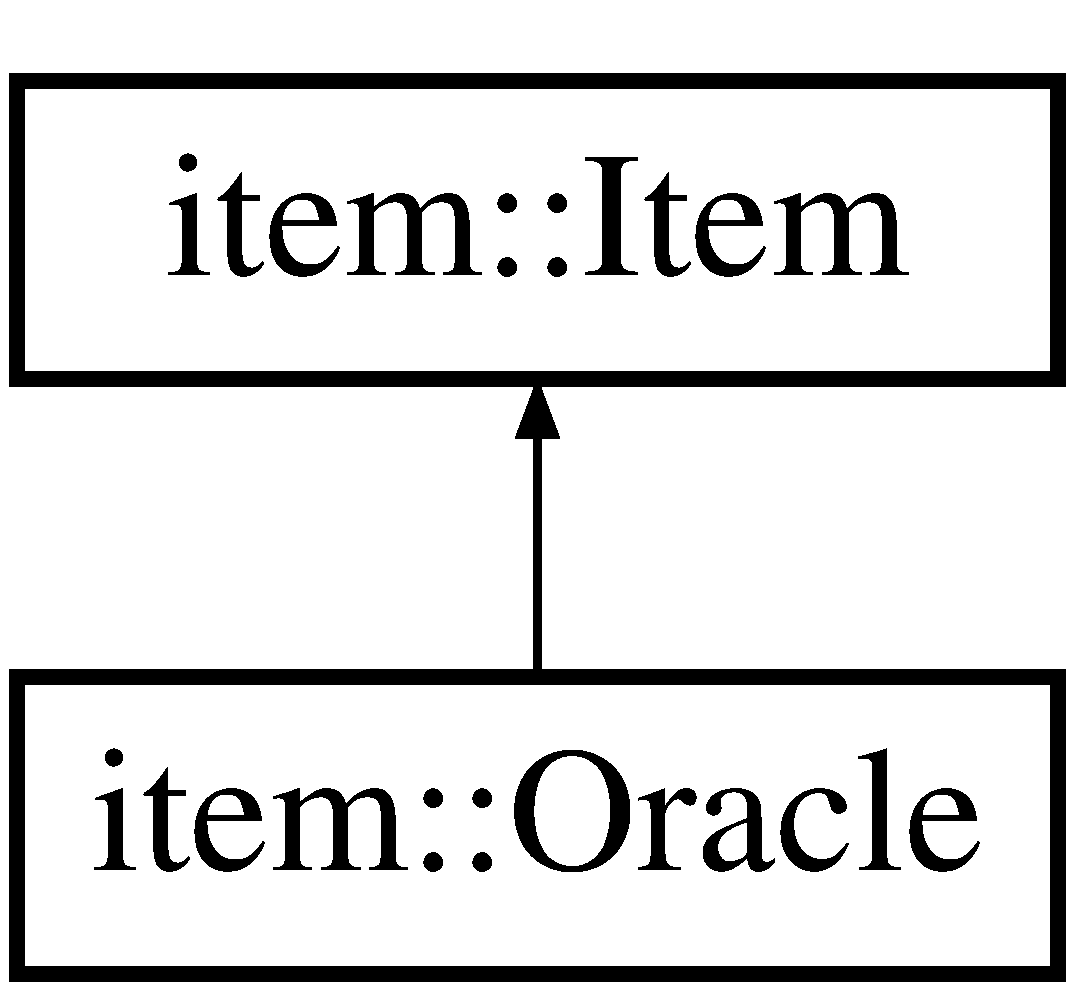
\includegraphics[height=2.000000cm]{classitem_1_1_oracle}
\end{center}
\end{figure}
\subsection*{Public Member Functions}
\begin{DoxyCompactItemize}
\item 
\mbox{\Hypertarget{classitem_1_1_oracle_aef8394c1370b0cf661b84ea454cff536}\label{classitem_1_1_oracle_aef8394c1370b0cf661b84ea454cff536}} 
{\bfseries Oracle} (\hyperlink{classtimeplane_1_1_moment}{Moment} first\+\_\+moment)
\item 
\hyperlink{classitem_1_1_effect}{Effect} \hyperlink{classitem_1_1_oracle_ade8c5db0ab73bfa61d5dbe2c9c405f5c}{View} (\hyperlink{classtimeplane_1_1_moment}{Moment} m) const
\begin{DoxyCompactList}\small\item\em View the effects of an item at a specific moment. \end{DoxyCompactList}\item 
Tagged\+Values \hyperlink{classitem_1_1_oracle_a78dd3984a5a0dae432c86e18520d7c46}{State\+Tagged\+Values} (\hyperlink{classtimeplane_1_1_moment}{Moment} m) const
\begin{DoxyCompactList}\small\item\em Virtual method to provide user-\/friendly tagged values. \end{DoxyCompactList}\end{DoxyCompactItemize}
\subsection*{Static Public Attributes}
\begin{DoxyCompactItemize}
\item 
static Item\+Type constexpr \hyperlink{classitem_1_1_oracle_a6905378f36854ca2ef63d403c95ede8f}{type} = Item\+Type\+::k\+Oracle
\begin{DoxyCompactList}\small\item\em An enum representation of the type of the item. \end{DoxyCompactList}\item 
\mbox{\Hypertarget{classitem_1_1_oracle_aefa06d76cc06f9a9f5b324806ca3bb37}\label{classitem_1_1_oracle_aefa06d76cc06f9a9f5b324806ca3bb37}} 
static int constexpr \hyperlink{classitem_1_1_oracle_aefa06d76cc06f9a9f5b324806ca3bb37}{k\+Unlock\+Requirement} = 45
\begin{DoxyCompactList}\small\item\em Energy requirement to unlock the item. \end{DoxyCompactList}\end{DoxyCompactItemize}
\subsection*{Protected Member Functions}
\begin{DoxyCompactItemize}
\item 
std\+::pair$<$ \hyperlink{classitem_1_1_effect}{Effect}, \hyperlink{classitem_1_1_item_properties}{Item\+Properties} $>$ \hyperlink{classitem_1_1_oracle_af765dd1df5a43de79539f9ce960854c0}{Step\+Impl} (\hyperlink{classtimeplane_1_1_moment}{Moment} curr, \hyperlink{classroundinfo_1_1_round_info_view}{Round\+Info\+View} const \&round\+\_\+info\+\_\+view, int energy\+\_\+input)
\begin{DoxyCompactList}\small\item\em Virtual method for computing the results of making a step. \end{DoxyCompactList}\item 
std\+::pair$<$ \hyperlink{classitem_1_1_effect}{Effect}, \hyperlink{classitem_1_1_item_properties}{Item\+Properties} $>$ \hyperlink{classitem_1_1_oracle_a9a8911eef902d4dcca95f111fda7c5d0}{Branch\+Impl} (\hyperlink{classtimeplane_1_1_moment}{Moment} curr, \hyperlink{classtimeplane_1_1_moment}{Moment} dest)
\begin{DoxyCompactList}\small\item\em Virtual method for computing the results of branching. \end{DoxyCompactList}\end{DoxyCompactItemize}
\subsection*{Additional Inherited Members}


\subsection{Detailed Description}
\hyperlink{classitem_1_1_item}{Item} that can make a player controllable. 

The player is made directly controllable when the \hyperlink{classitem_1_1_oracle}{Oracle} is activated, regardless of what timeline the activation has occurred in. 

\subsection{Member Function Documentation}
\mbox{\Hypertarget{classitem_1_1_oracle_ade8c5db0ab73bfa61d5dbe2c9c405f5c}\label{classitem_1_1_oracle_ade8c5db0ab73bfa61d5dbe2c9c405f5c}} 
\index{item\+::\+Oracle@{item\+::\+Oracle}!View@{View}}
\index{View@{View}!item\+::\+Oracle@{item\+::\+Oracle}}
\subsubsection{\texorpdfstring{View()}{View()}}
{\footnotesize\ttfamily \hyperlink{classitem_1_1_effect}{Effect} Oracle\+::\+View (\begin{DoxyParamCaption}\item[{\hyperlink{classtimeplane_1_1_moment}{Moment}}]{m }\end{DoxyParamCaption}) const\hspace{0.3cm}{\ttfamily [virtual]}}



View the effects of an item at a specific moment. 

This call must be a pure function not only of the provided moment, but also be a function of {\ttfamily Get\+Properties(m)}. 
\begin{DoxyParams}{Parameters}
{\em m} & The moment to query. \\
\hline
\end{DoxyParams}
\begin{DoxyReturn}{Returns}
The effects granted by the item at the specified moment. 
\end{DoxyReturn}

\begin{DoxyExceptions}{Exceptions}
{\em std\+::out\+\_\+of\+\_\+range} & Potentially thrown by subclasses. \\
\hline
\end{DoxyExceptions}


Implements \hyperlink{classitem_1_1_item_a7d2b010a27fec55e04a56e7c4fca7837}{item\+::\+Item}.

\mbox{\Hypertarget{classitem_1_1_oracle_a78dd3984a5a0dae432c86e18520d7c46}\label{classitem_1_1_oracle_a78dd3984a5a0dae432c86e18520d7c46}} 
\index{item\+::\+Oracle@{item\+::\+Oracle}!State\+Tagged\+Values@{State\+Tagged\+Values}}
\index{State\+Tagged\+Values@{State\+Tagged\+Values}!item\+::\+Oracle@{item\+::\+Oracle}}
\subsubsection{\texorpdfstring{State\+Tagged\+Values()}{StateTaggedValues()}}
{\footnotesize\ttfamily Tagged\+Values Oracle\+::\+State\+Tagged\+Values (\begin{DoxyParamCaption}\item[{\hyperlink{classtimeplane_1_1_moment}{Moment}}]{m }\end{DoxyParamCaption}) const\hspace{0.3cm}{\ttfamily [virtual]}}



Virtual method to provide user-\/friendly tagged values. 

The tags are used as a user-\/friendly indication of the internal state of the item at a given moment without revealing implementation detail, and can also be used to attach specific meaning to the abstract lockdown and cooldown values associated with all items. 
\begin{DoxyParams}{Parameters}
{\em m} & The moment to query. \\
\hline
\end{DoxyParams}
\begin{DoxyReturn}{Returns}
A group of tagged values describing the state of an item. 
\end{DoxyReturn}


Implements \hyperlink{classitem_1_1_item_a8410ab3ab75e65360eddb4f6bd3cceff}{item\+::\+Item}.

\mbox{\Hypertarget{classitem_1_1_oracle_af765dd1df5a43de79539f9ce960854c0}\label{classitem_1_1_oracle_af765dd1df5a43de79539f9ce960854c0}} 
\index{item\+::\+Oracle@{item\+::\+Oracle}!Step\+Impl@{Step\+Impl}}
\index{Step\+Impl@{Step\+Impl}!item\+::\+Oracle@{item\+::\+Oracle}}
\subsubsection{\texorpdfstring{Step\+Impl()}{StepImpl()}}
{\footnotesize\ttfamily std\+::pair$<$ \hyperlink{classitem_1_1_effect}{Effect}, \hyperlink{classitem_1_1_item_properties}{Item\+Properties} $>$ Oracle\+::\+Step\+Impl (\begin{DoxyParamCaption}\item[{\hyperlink{classtimeplane_1_1_moment}{Moment}}]{curr,  }\item[{\hyperlink{classroundinfo_1_1_round_info_view}{Round\+Info\+View} const \&}]{turn\+\_\+data,  }\item[{int}]{energy\+\_\+input }\end{DoxyParamCaption})\hspace{0.3cm}{\ttfamily [protected]}, {\ttfamily [virtual]}}



Virtual method for computing the results of making a step. 


\begin{DoxyParams}{Parameters}
{\em curr} & The current moment before the step. \\
\hline
{\em turn\+\_\+data} & The information about the turn just played. \\
\hline
\end{DoxyParams}
\begin{DoxyReturn}{Returns}
The effects granted by the item for the next round, and the properties of the item for the next round. 
\end{DoxyReturn}


Implements \hyperlink{classitem_1_1_item_a90df61c8a2a20144eb1100af5fb2d464}{item\+::\+Item}.

\mbox{\Hypertarget{classitem_1_1_oracle_a9a8911eef902d4dcca95f111fda7c5d0}\label{classitem_1_1_oracle_a9a8911eef902d4dcca95f111fda7c5d0}} 
\index{item\+::\+Oracle@{item\+::\+Oracle}!Branch\+Impl@{Branch\+Impl}}
\index{Branch\+Impl@{Branch\+Impl}!item\+::\+Oracle@{item\+::\+Oracle}}
\subsubsection{\texorpdfstring{Branch\+Impl()}{BranchImpl()}}
{\footnotesize\ttfamily std\+::pair$<$ \hyperlink{classitem_1_1_effect}{Effect}, \hyperlink{classitem_1_1_item_properties}{Item\+Properties} $>$ Oracle\+::\+Branch\+Impl (\begin{DoxyParamCaption}\item[{\hyperlink{classtimeplane_1_1_moment}{Moment}}]{curr,  }\item[{\hyperlink{classtimeplane_1_1_moment}{Moment}}]{dest }\end{DoxyParamCaption})\hspace{0.3cm}{\ttfamily [protected]}, {\ttfamily [virtual]}}



Virtual method for computing the results of branching. 


\begin{DoxyParams}{Parameters}
{\em curr} & The current moment before branching. \\
\hline
{\em dest} & The destination moment to reach. \\
\hline
\end{DoxyParams}
\begin{DoxyReturn}{Returns}
The effects granted by the item for the next round, and the properties of the item for the next round. 
\end{DoxyReturn}


Implements \hyperlink{classitem_1_1_item_afef6bdd5c1c734c67122e4118e9e1930}{item\+::\+Item}.



\subsection{Member Data Documentation}
\mbox{\Hypertarget{classitem_1_1_oracle_a6905378f36854ca2ef63d403c95ede8f}\label{classitem_1_1_oracle_a6905378f36854ca2ef63d403c95ede8f}} 
\index{item\+::\+Oracle@{item\+::\+Oracle}!type@{type}}
\index{type@{type}!item\+::\+Oracle@{item\+::\+Oracle}}
\subsubsection{\texorpdfstring{type}{type}}
{\footnotesize\ttfamily Item\+Type constexpr item\+::\+Oracle\+::type = Item\+Type\+::k\+Oracle\hspace{0.3cm}{\ttfamily [static]}}



An enum representation of the type of the item. 

The value of the enum is a unique value for each item, and are consecutive starting at 0 across all items. 

The documentation for this class was generated from the following files\+:\begin{DoxyCompactItemize}
\item 
K\+:/\+Personal Projects/\+Antitelephone\+Q\+T/src/oracle.\+hpp\item 
K\+:/\+Personal Projects/\+Antitelephone\+Q\+T/src/oracle.\+cpp\end{DoxyCompactItemize}

\hypertarget{class_query_result}{}\section{Query\+Result Class Reference}
\label{class_query_result}\index{Query\+Result@{Query\+Result}}


A class representing a server\textquotesingle{}s response to a query.  




{\ttfamily \#include $<$queryresult.\+hpp$>$}

\subsection*{Public Member Functions}
\begin{DoxyCompactItemize}
\item 
\hyperlink{class_query_result_a2bcdccec574314df85c4bff6611c215b}{Query\+Result} (bool \hyperlink{class_query_result_ae1b66d19c66ed5c97dd3322c3c721c82}{success}, std\+::string const \&\hyperlink{class_query_result_a3d238ce0ccc659d2918dac0479937d3c}{response\+\_\+tag}=\char`\"{}\char`\"{})
\begin{DoxyCompactList}\small\item\em Constructor. \end{DoxyCompactList}\item 
\mbox{\Hypertarget{class_query_result_a280533eecc3453bb2e65119070cc9fc7}\label{class_query_result_a280533eecc3453bb2e65119070cc9fc7}} 
\hyperlink{class_query_result_a280533eecc3453bb2e65119070cc9fc7}{operator bool} () const noexcept
\begin{DoxyCompactList}\small\item\em Implicit cast to the underlying success value. \end{DoxyCompactList}\item 
bool \hyperlink{class_query_result_ae1b66d19c66ed5c97dd3322c3c721c82}{success} () const noexcept
\begin{DoxyCompactList}\small\item\em Accessor for the success value. \end{DoxyCompactList}\item 
std\+::string const  \& \hyperlink{class_query_result_a3d238ce0ccc659d2918dac0479937d3c}{response\+\_\+tag} () const noexcept
\begin{DoxyCompactList}\small\item\em Accessor for the response tag. \end{DoxyCompactList}\end{DoxyCompactItemize}


\subsection{Detailed Description}
A class representing a server\textquotesingle{}s response to a query. 

\subsection{Constructor \& Destructor Documentation}
\mbox{\Hypertarget{class_query_result_a2bcdccec574314df85c4bff6611c215b}\label{class_query_result_a2bcdccec574314df85c4bff6611c215b}} 
\index{Query\+Result@{Query\+Result}!Query\+Result@{Query\+Result}}
\index{Query\+Result@{Query\+Result}!Query\+Result@{Query\+Result}}
\subsubsection{\texorpdfstring{Query\+Result()}{QueryResult()}}
{\footnotesize\ttfamily Query\+Result\+::\+Query\+Result (\begin{DoxyParamCaption}\item[{bool}]{success,  }\item[{std\+::string const \&}]{response\+\_\+tag = {\ttfamily \char`\"{}\char`\"{}} }\end{DoxyParamCaption})\hspace{0.3cm}{\ttfamily [inline]}}



Constructor. 


\begin{DoxyParams}{Parameters}
{\em success} & Whether the query was a success. \\
\hline
{\em response\+\_\+tag} & String tag associated with the response. \\
\hline
\end{DoxyParams}


\subsection{Member Function Documentation}
\mbox{\Hypertarget{class_query_result_ae1b66d19c66ed5c97dd3322c3c721c82}\label{class_query_result_ae1b66d19c66ed5c97dd3322c3c721c82}} 
\index{Query\+Result@{Query\+Result}!success@{success}}
\index{success@{success}!Query\+Result@{Query\+Result}}
\subsubsection{\texorpdfstring{success()}{success()}}
{\footnotesize\ttfamily bool Query\+Result\+::success (\begin{DoxyParamCaption}{ }\end{DoxyParamCaption}) const\hspace{0.3cm}{\ttfamily [inline]}, {\ttfamily [noexcept]}}



Accessor for the success value. 

\begin{DoxyReturn}{Returns}
Whether the query was a success. 
\end{DoxyReturn}
\mbox{\Hypertarget{class_query_result_a3d238ce0ccc659d2918dac0479937d3c}\label{class_query_result_a3d238ce0ccc659d2918dac0479937d3c}} 
\index{Query\+Result@{Query\+Result}!response\+\_\+tag@{response\+\_\+tag}}
\index{response\+\_\+tag@{response\+\_\+tag}!Query\+Result@{Query\+Result}}
\subsubsection{\texorpdfstring{response\+\_\+tag()}{response\_tag()}}
{\footnotesize\ttfamily std\+::string const\& Query\+Result\+::response\+\_\+tag (\begin{DoxyParamCaption}{ }\end{DoxyParamCaption}) const\hspace{0.3cm}{\ttfamily [inline]}, {\ttfamily [noexcept]}}



Accessor for the response tag. 

\begin{DoxyReturn}{Returns}
Tag associated with the response. 
\end{DoxyReturn}


The documentation for this class was generated from the following file\+:\begin{DoxyCompactItemize}
\item 
K\+:/\+Personal Projects/\+Antitelephone\+Q\+T/src/queryresult.\+hpp\end{DoxyCompactItemize}

\hypertarget{classroundinfo_1_1_round_info}{}\section{roundinfo\+:\+:Round\+Info Class Reference}
\label{classroundinfo_1_1_round_info}\index{roundinfo\+::\+Round\+Info@{roundinfo\+::\+Round\+Info}}


A representation of data relevant to a single round of gameplay.  




{\ttfamily \#include $<$roundinfo.\+hpp$>$}

\subsection*{Public Member Functions}
\begin{DoxyCompactItemize}
\item 
\hyperlink{classroundinfo_1_1_round_info_abf54268ebef648dc57353dd2fd6374b5}{Round\+Info} (int \hyperlink{classroundinfo_1_1_round_info_a004757e903e2b24d73d746040f8afd42}{num\+\_\+players})
\begin{DoxyCompactList}\small\item\em Constructor. \end{DoxyCompactList}\item 
int \hyperlink{classroundinfo_1_1_round_info_a004757e903e2b24d73d746040f8afd42}{num\+\_\+players} () const noexcept
\begin{DoxyCompactList}\small\item\em Accessor for the number of players in the game. \end{DoxyCompactList}\item 
int \hyperlink{classroundinfo_1_1_round_info_aab20da577e7b2741d4e478b6d353324c}{Location} (int player, int viewing\+\_\+player) const
\begin{DoxyCompactList}\small\item\em Accessor for the location of a player. \end{DoxyCompactList}\item 
int \hyperlink{classroundinfo_1_1_round_info_a2b6c4500a8076cb24f83591f05b99fba}{Damage\+Received} (int player, int viewing\+\_\+player) const
\begin{DoxyCompactList}\small\item\em Accessor for the damage a player received. \end{DoxyCompactList}\item 
int \hyperlink{classroundinfo_1_1_round_info_accb2ab979f9fe090cf03753ed1c78e0a}{Health\+Remaining} (int player, int viewing\+\_\+player) const
\begin{DoxyCompactList}\small\item\em Accessor for the health a player has remaining. \end{DoxyCompactList}\item 
bool \hyperlink{classroundinfo_1_1_round_info_a03a7ee40677506160aef2766929e6105}{Active} (int player) const
\begin{DoxyCompactList}\small\item\em Accessor for whether a player is active. \end{DoxyCompactList}\item 
\hyperlink{class_symmetric_bit_matrix}{Symmetric\+Bit\+Matrix} const  \& \hyperlink{classroundinfo_1_1_round_info_a0944e6bf6facb52e9955695ea0b3feb3}{calliance\+\_\+data} () const noexcept
\begin{DoxyCompactList}\small\item\em Accessor to view the alliance data. \end{DoxyCompactList}\item 
Int\+Iterator \hyperlink{classroundinfo_1_1_round_info_ab9e17ca5d68f9981862cbf540cc0b297}{Location\+Iterator} () noexcept
\begin{DoxyCompactList}\small\item\em Iterator to modify the location data. \end{DoxyCompactList}\item 
Int\+Iterator \hyperlink{classroundinfo_1_1_round_info_a94ea1a09ae7680e74188296aef0b0d63}{Damage\+Received\+Iterator} () noexcept
\begin{DoxyCompactList}\small\item\em Iterator to modify the damage received data. \end{DoxyCompactList}\item 
Int\+Iterator \hyperlink{classroundinfo_1_1_round_info_a3a81f2d87bea27339f035201f1887423}{Health\+Remaining\+Iterator} () noexcept
\begin{DoxyCompactList}\small\item\em Iterator to modify the health remaining data. \end{DoxyCompactList}\item 
void \hyperlink{classroundinfo_1_1_round_info_a28d85479753dae18a6b2a27d048d2973}{Set\+Active} (int player, bool value)
\begin{DoxyCompactList}\small\item\em Mutator to set the active status of a player. \end{DoxyCompactList}\item 
\hyperlink{class_symmetric_bit_matrix}{Symmetric\+Bit\+Matrix} \& \hyperlink{classroundinfo_1_1_round_info_a9d5ae58298d3acd11377da7992235762}{alliance\+\_\+data} () noexcept
\begin{DoxyCompactList}\small\item\em Accessor to modify the alliance data. \end{DoxyCompactList}\end{DoxyCompactItemize}
\subsection*{Static Public Attributes}
\begin{DoxyCompactItemize}
\item 
\mbox{\Hypertarget{classroundinfo_1_1_round_info_a6a7ac5df8cced5aac3c30a98f88df3d9}\label{classroundinfo_1_1_round_info_a6a7ac5df8cced5aac3c30a98f88df3d9}} 
static int constexpr {\bfseries k\+Unknown} = -\/1
\item 
\mbox{\Hypertarget{classroundinfo_1_1_round_info_a316f9f9173bcbf923181a84deb70c4d0}\label{classroundinfo_1_1_round_info_a316f9f9173bcbf923181a84deb70c4d0}} 
static int constexpr {\bfseries k\+Graveyard\+Location} = -\/2
\item 
\mbox{\Hypertarget{classroundinfo_1_1_round_info_a29eb9d113e033613762e50e1aaf63290}\label{classroundinfo_1_1_round_info_a29eb9d113e033613762e50e1aaf63290}} 
static int constexpr {\bfseries k\+Omniscient\+Viewer} = -\/1
\end{DoxyCompactItemize}


\subsection{Detailed Description}
A representation of data relevant to a single round of gameplay. 

Information about the players as well as any interactions between players in a single round of gameplay is stored in this instance. Information about the items held by players is  not stored in this instance. Using alliance and encounter data, the instance also enforces the privacy of certain player information from other viewers. 

\subsection{Constructor \& Destructor Documentation}
\mbox{\Hypertarget{classroundinfo_1_1_round_info_abf54268ebef648dc57353dd2fd6374b5}\label{classroundinfo_1_1_round_info_abf54268ebef648dc57353dd2fd6374b5}} 
\index{roundinfo\+::\+Round\+Info@{roundinfo\+::\+Round\+Info}!Round\+Info@{Round\+Info}}
\index{Round\+Info@{Round\+Info}!roundinfo\+::\+Round\+Info@{roundinfo\+::\+Round\+Info}}
\subsubsection{\texorpdfstring{Round\+Info()}{RoundInfo()}}
{\footnotesize\ttfamily Round\+Info\+::\+Round\+Info (\begin{DoxyParamCaption}\item[{int}]{num\+\_\+players }\end{DoxyParamCaption})}



Constructor. 

The alliances of the players are by default set such that each player is not allied to any different player (though they are trivially allied to themselves). Initial values of locations, health data and player active status are unspecified. 
\begin{DoxyParams}{Parameters}
{\em num\+\_\+players} & The number of players in the game. \\
\hline
\end{DoxyParams}


\subsection{Member Function Documentation}
\mbox{\Hypertarget{classroundinfo_1_1_round_info_a004757e903e2b24d73d746040f8afd42}\label{classroundinfo_1_1_round_info_a004757e903e2b24d73d746040f8afd42}} 
\index{roundinfo\+::\+Round\+Info@{roundinfo\+::\+Round\+Info}!num\+\_\+players@{num\+\_\+players}}
\index{num\+\_\+players@{num\+\_\+players}!roundinfo\+::\+Round\+Info@{roundinfo\+::\+Round\+Info}}
\subsubsection{\texorpdfstring{num\+\_\+players()}{num\_players()}}
{\footnotesize\ttfamily int roundinfo\+::\+Round\+Info\+::num\+\_\+players (\begin{DoxyParamCaption}{ }\end{DoxyParamCaption}) const\hspace{0.3cm}{\ttfamily [inline]}, {\ttfamily [noexcept]}}



Accessor for the number of players in the game. 

\begin{DoxyReturn}{Returns}
The number of players in the game. 
\end{DoxyReturn}
\mbox{\Hypertarget{classroundinfo_1_1_round_info_aab20da577e7b2741d4e478b6d353324c}\label{classroundinfo_1_1_round_info_aab20da577e7b2741d4e478b6d353324c}} 
\index{roundinfo\+::\+Round\+Info@{roundinfo\+::\+Round\+Info}!Location@{Location}}
\index{Location@{Location}!roundinfo\+::\+Round\+Info@{roundinfo\+::\+Round\+Info}}
\subsubsection{\texorpdfstring{Location()}{Location()}}
{\footnotesize\ttfamily int Round\+Info\+::\+Location (\begin{DoxyParamCaption}\item[{int}]{player,  }\item[{int}]{viewing\+\_\+player }\end{DoxyParamCaption}) const}



Accessor for the location of a player. 


\begin{DoxyParams}{Parameters}
{\em player} & The player ID to query. \\
\hline
{\em viewing\+\_\+player} & The player attempting to make the query. \\
\hline
\end{DoxyParams}
\begin{DoxyReturn}{Returns}
The location of the player queried, or {\ttfamily k\+Unknown} if the player making the query is not authorized to know. 
\end{DoxyReturn}

\begin{DoxyExceptions}{Exceptions}
{\em std\+::out\+\_\+of\+\_\+range} & If no player with the specified ID exists. \\
\hline
\end{DoxyExceptions}
\mbox{\Hypertarget{classroundinfo_1_1_round_info_a2b6c4500a8076cb24f83591f05b99fba}\label{classroundinfo_1_1_round_info_a2b6c4500a8076cb24f83591f05b99fba}} 
\index{roundinfo\+::\+Round\+Info@{roundinfo\+::\+Round\+Info}!Damage\+Received@{Damage\+Received}}
\index{Damage\+Received@{Damage\+Received}!roundinfo\+::\+Round\+Info@{roundinfo\+::\+Round\+Info}}
\subsubsection{\texorpdfstring{Damage\+Received()}{DamageReceived()}}
{\footnotesize\ttfamily int Round\+Info\+::\+Damage\+Received (\begin{DoxyParamCaption}\item[{int}]{player,  }\item[{int}]{viewing\+\_\+player }\end{DoxyParamCaption}) const}



Accessor for the damage a player received. 

This value is distinct from the change in health across moments because of potential shielding effects from items. 
\begin{DoxyParams}{Parameters}
{\em player} & The player ID to query. \\
\hline
{\em viewing\+\_\+player} & The player attempting to make the query. \\
\hline
\end{DoxyParams}
\begin{DoxyReturn}{Returns}
The damage received of the player queried, or {\ttfamily k\+Unknown} if the player making the query is not authorized to know. 
\end{DoxyReturn}

\begin{DoxyExceptions}{Exceptions}
{\em std\+::out\+\_\+of\+\_\+range} & If no player with the specified ID exists. \\
\hline
\end{DoxyExceptions}
\mbox{\Hypertarget{classroundinfo_1_1_round_info_accb2ab979f9fe090cf03753ed1c78e0a}\label{classroundinfo_1_1_round_info_accb2ab979f9fe090cf03753ed1c78e0a}} 
\index{roundinfo\+::\+Round\+Info@{roundinfo\+::\+Round\+Info}!Health\+Remaining@{Health\+Remaining}}
\index{Health\+Remaining@{Health\+Remaining}!roundinfo\+::\+Round\+Info@{roundinfo\+::\+Round\+Info}}
\subsubsection{\texorpdfstring{Health\+Remaining()}{HealthRemaining()}}
{\footnotesize\ttfamily int Round\+Info\+::\+Health\+Remaining (\begin{DoxyParamCaption}\item[{int}]{player,  }\item[{int}]{viewing\+\_\+player }\end{DoxyParamCaption}) const}



Accessor for the health a player has remaining. 


\begin{DoxyParams}{Parameters}
{\em player} & The player ID to query. \\
\hline
{\em viewing\+\_\+player} & The player attempting to make the query. \\
\hline
\end{DoxyParams}
\begin{DoxyReturn}{Returns}
The health remaining of the player queried, or {\ttfamily k\+Unknown} if the player making the query is not authorized to know. 
\end{DoxyReturn}

\begin{DoxyExceptions}{Exceptions}
{\em std\+::out\+\_\+of\+\_\+range} & If no player with the specified ID exists. \\
\hline
\end{DoxyExceptions}
\mbox{\Hypertarget{classroundinfo_1_1_round_info_a03a7ee40677506160aef2766929e6105}\label{classroundinfo_1_1_round_info_a03a7ee40677506160aef2766929e6105}} 
\index{roundinfo\+::\+Round\+Info@{roundinfo\+::\+Round\+Info}!Active@{Active}}
\index{Active@{Active}!roundinfo\+::\+Round\+Info@{roundinfo\+::\+Round\+Info}}
\subsubsection{\texorpdfstring{Active()}{Active()}}
{\footnotesize\ttfamily bool Round\+Info\+::\+Active (\begin{DoxyParamCaption}\item[{int}]{player }\end{DoxyParamCaption}) const}



Accessor for whether a player is active. 


\begin{DoxyParams}{Parameters}
{\em player} & The player ID to query. \\
\hline
\end{DoxyParams}
\begin{DoxyReturn}{Returns}
Whether the player queried is active. 
\end{DoxyReturn}

\begin{DoxyExceptions}{Exceptions}
{\em std\+::out\+\_\+of\+\_\+range} & If no player with the specified ID exists. \\
\hline
\end{DoxyExceptions}
\mbox{\Hypertarget{classroundinfo_1_1_round_info_a0944e6bf6facb52e9955695ea0b3feb3}\label{classroundinfo_1_1_round_info_a0944e6bf6facb52e9955695ea0b3feb3}} 
\index{roundinfo\+::\+Round\+Info@{roundinfo\+::\+Round\+Info}!calliance\+\_\+data@{calliance\+\_\+data}}
\index{calliance\+\_\+data@{calliance\+\_\+data}!roundinfo\+::\+Round\+Info@{roundinfo\+::\+Round\+Info}}
\subsubsection{\texorpdfstring{calliance\+\_\+data()}{calliance\_data()}}
{\footnotesize\ttfamily \hyperlink{class_symmetric_bit_matrix}{Symmetric\+Bit\+Matrix} const\& roundinfo\+::\+Round\+Info\+::calliance\+\_\+data (\begin{DoxyParamCaption}{ }\end{DoxyParamCaption}) const\hspace{0.3cm}{\ttfamily [inline]}, {\ttfamily [noexcept]}}



Accessor to view the alliance data. 

\begin{DoxyReturn}{Returns}
A constant reference to the alliance data. 
\end{DoxyReturn}
\mbox{\Hypertarget{classroundinfo_1_1_round_info_ab9e17ca5d68f9981862cbf540cc0b297}\label{classroundinfo_1_1_round_info_ab9e17ca5d68f9981862cbf540cc0b297}} 
\index{roundinfo\+::\+Round\+Info@{roundinfo\+::\+Round\+Info}!Location\+Iterator@{Location\+Iterator}}
\index{Location\+Iterator@{Location\+Iterator}!roundinfo\+::\+Round\+Info@{roundinfo\+::\+Round\+Info}}
\subsubsection{\texorpdfstring{Location\+Iterator()}{LocationIterator()}}
{\footnotesize\ttfamily Int\+Iterator roundinfo\+::\+Round\+Info\+::\+Location\+Iterator (\begin{DoxyParamCaption}{ }\end{DoxyParamCaption})\hspace{0.3cm}{\ttfamily [inline]}, {\ttfamily [noexcept]}}



Iterator to modify the location data. 

\begin{DoxyReturn}{Returns}
A random access iterator to the location data. 
\end{DoxyReturn}
\mbox{\Hypertarget{classroundinfo_1_1_round_info_a94ea1a09ae7680e74188296aef0b0d63}\label{classroundinfo_1_1_round_info_a94ea1a09ae7680e74188296aef0b0d63}} 
\index{roundinfo\+::\+Round\+Info@{roundinfo\+::\+Round\+Info}!Damage\+Received\+Iterator@{Damage\+Received\+Iterator}}
\index{Damage\+Received\+Iterator@{Damage\+Received\+Iterator}!roundinfo\+::\+Round\+Info@{roundinfo\+::\+Round\+Info}}
\subsubsection{\texorpdfstring{Damage\+Received\+Iterator()}{DamageReceivedIterator()}}
{\footnotesize\ttfamily Int\+Iterator roundinfo\+::\+Round\+Info\+::\+Damage\+Received\+Iterator (\begin{DoxyParamCaption}{ }\end{DoxyParamCaption})\hspace{0.3cm}{\ttfamily [inline]}, {\ttfamily [noexcept]}}



Iterator to modify the damage received data. 

\begin{DoxyReturn}{Returns}
A random access iterator to the damage received data. 
\end{DoxyReturn}
\mbox{\Hypertarget{classroundinfo_1_1_round_info_a3a81f2d87bea27339f035201f1887423}\label{classroundinfo_1_1_round_info_a3a81f2d87bea27339f035201f1887423}} 
\index{roundinfo\+::\+Round\+Info@{roundinfo\+::\+Round\+Info}!Health\+Remaining\+Iterator@{Health\+Remaining\+Iterator}}
\index{Health\+Remaining\+Iterator@{Health\+Remaining\+Iterator}!roundinfo\+::\+Round\+Info@{roundinfo\+::\+Round\+Info}}
\subsubsection{\texorpdfstring{Health\+Remaining\+Iterator()}{HealthRemainingIterator()}}
{\footnotesize\ttfamily Int\+Iterator roundinfo\+::\+Round\+Info\+::\+Health\+Remaining\+Iterator (\begin{DoxyParamCaption}{ }\end{DoxyParamCaption})\hspace{0.3cm}{\ttfamily [inline]}, {\ttfamily [noexcept]}}



Iterator to modify the health remaining data. 

\begin{DoxyReturn}{Returns}
A random access iterator to the health remaining data. 
\end{DoxyReturn}
\mbox{\Hypertarget{classroundinfo_1_1_round_info_a28d85479753dae18a6b2a27d048d2973}\label{classroundinfo_1_1_round_info_a28d85479753dae18a6b2a27d048d2973}} 
\index{roundinfo\+::\+Round\+Info@{roundinfo\+::\+Round\+Info}!Set\+Active@{Set\+Active}}
\index{Set\+Active@{Set\+Active}!roundinfo\+::\+Round\+Info@{roundinfo\+::\+Round\+Info}}
\subsubsection{\texorpdfstring{Set\+Active()}{SetActive()}}
{\footnotesize\ttfamily void Round\+Info\+::\+Set\+Active (\begin{DoxyParamCaption}\item[{int}]{player,  }\item[{bool}]{value }\end{DoxyParamCaption})}



Mutator to set the active status of a player. 


\begin{DoxyParams}{Parameters}
{\em player} & The player whose active status is modified. \\
\hline
{\em value} & The active status value to set. \\
\hline
\end{DoxyParams}

\begin{DoxyExceptions}{Exceptions}
{\em std\+::out\+\_\+of\+\_\+range} & If no player with the specified ID exists. \\
\hline
\end{DoxyExceptions}
\mbox{\Hypertarget{classroundinfo_1_1_round_info_a9d5ae58298d3acd11377da7992235762}\label{classroundinfo_1_1_round_info_a9d5ae58298d3acd11377da7992235762}} 
\index{roundinfo\+::\+Round\+Info@{roundinfo\+::\+Round\+Info}!alliance\+\_\+data@{alliance\+\_\+data}}
\index{alliance\+\_\+data@{alliance\+\_\+data}!roundinfo\+::\+Round\+Info@{roundinfo\+::\+Round\+Info}}
\subsubsection{\texorpdfstring{alliance\+\_\+data()}{alliance\_data()}}
{\footnotesize\ttfamily \hyperlink{class_symmetric_bit_matrix}{Symmetric\+Bit\+Matrix}\& roundinfo\+::\+Round\+Info\+::alliance\+\_\+data (\begin{DoxyParamCaption}{ }\end{DoxyParamCaption})\hspace{0.3cm}{\ttfamily [inline]}, {\ttfamily [noexcept]}}



Accessor to modify the alliance data. 

\begin{DoxyReturn}{Returns}
A mutable reference to the alliance data. 
\end{DoxyReturn}


The documentation for this class was generated from the following files\+:\begin{DoxyCompactItemize}
\item 
K\+:/\+Personal Projects/\+Antitelephone\+Q\+T/src/roundinfo.\+hpp\item 
K\+:/\+Personal Projects/\+Antitelephone\+Q\+T/src/roundinfo.\+cpp\end{DoxyCompactItemize}

\hypertarget{classroundinfo_1_1_round_info_view}{}\section{roundinfo\+:\+:Round\+Info\+View Class Reference}
\label{classroundinfo_1_1_round_info_view}\index{roundinfo\+::\+Round\+Info\+View@{roundinfo\+::\+Round\+Info\+View}}


Information contained in {\ttfamily \hyperlink{classroundinfo_1_1_round_info}{Round\+Info}} as seen from a single player.  




{\ttfamily \#include $<$roundinfoview.\+hpp$>$}

\subsection*{Public Member Functions}
\begin{DoxyCompactItemize}
\item 
\hyperlink{classroundinfo_1_1_round_info_view_a29937c9ac9cd71b7edd10f612ce76c91}{Round\+Info\+View} ()
\begin{DoxyCompactList}\small\item\em Default constructor. \end{DoxyCompactList}\item 
\hyperlink{classroundinfo_1_1_round_info_view_a8c5bca173f30cc869505c36baf04ebaa}{Round\+Info\+View} (\hyperlink{classroundinfo_1_1_round_info}{Round\+Info} const \&source, int \hyperlink{classroundinfo_1_1_round_info_view_acb1e4edcbe9b01f59ba26542f528ba24}{player}, bool location\+\_\+omniscience=false)
\begin{DoxyCompactList}\small\item\em Constructor. \end{DoxyCompactList}\item 
int \hyperlink{classroundinfo_1_1_round_info_view_acb1e4edcbe9b01f59ba26542f528ba24}{player} () const noexcept
\begin{DoxyCompactList}\small\item\em Accessor for the ID of the player that the view centers from. \end{DoxyCompactList}\item 
int \hyperlink{classroundinfo_1_1_round_info_view_a05f42a982570552bbeb8c330e62437ad}{Location} (int \hyperlink{classroundinfo_1_1_round_info_view_acb1e4edcbe9b01f59ba26542f528ba24}{player}) const noexcept
\begin{DoxyCompactList}\small\item\em Accessor for the location of another player. \end{DoxyCompactList}\item 
int \hyperlink{classroundinfo_1_1_round_info_view_ac2d60e02ab84297d958b5b5caa653c7b}{Damage\+Received} (int \hyperlink{classroundinfo_1_1_round_info_view_acb1e4edcbe9b01f59ba26542f528ba24}{player}) const noexcept
\begin{DoxyCompactList}\small\item\em Accessor for the health remaining of another player. \end{DoxyCompactList}\item 
int \hyperlink{classroundinfo_1_1_round_info_view_a5b7dd1135b438e04017ad0a3bcc4034a}{Health\+Remaining} (int \hyperlink{classroundinfo_1_1_round_info_view_acb1e4edcbe9b01f59ba26542f528ba24}{player}) const noexcept
\begin{DoxyCompactList}\small\item\em Accessor for the health remaining of another player. \end{DoxyCompactList}\item 
Bit\+Set const  \& \hyperlink{classroundinfo_1_1_round_info_view_af00b23d7a3f2fa21fd3cbba1f71e0fd4}{allies} () const noexcept
\begin{DoxyCompactList}\small\item\em Accessor for the set of allies the player has. \end{DoxyCompactList}\item 
bool \hyperlink{classroundinfo_1_1_round_info_view_a1ff1802f7ab8e24008f02bbc0169a160}{active} () const noexcept
\begin{DoxyCompactList}\small\item\em Accessor for whether the player is actively in control. \end{DoxyCompactList}\item 
{\footnotesize template$<$typename Archive $>$ }\\void \hyperlink{classroundinfo_1_1_round_info_view_a101e6ee624aacfa8dd110aea67e67538}{serialize} (Archive \&ar, unsigned int const version)
\begin{DoxyCompactList}\small\item\em Serialization function. \end{DoxyCompactList}\end{DoxyCompactItemize}
\subsection*{Friends}
\begin{DoxyCompactItemize}
\item 
\mbox{\Hypertarget{classroundinfo_1_1_round_info_view_ac98d07dd8f7b70e16ccb9a01abf56b9c}\label{classroundinfo_1_1_round_info_view_ac98d07dd8f7b70e16ccb9a01abf56b9c}} 
class {\bfseries boost\+::serialization\+::access}
\end{DoxyCompactItemize}


\subsection{Detailed Description}
Information contained in {\ttfamily \hyperlink{classroundinfo_1_1_round_info}{Round\+Info}} as seen from a single player. 

Any information that a player is unauthorized to see is reported as {\ttfamily Round\+Info\+::k\+Unknown}. Instances of this class can be serialized. 

\subsection{Constructor \& Destructor Documentation}
\mbox{\Hypertarget{classroundinfo_1_1_round_info_view_a29937c9ac9cd71b7edd10f612ce76c91}\label{classroundinfo_1_1_round_info_view_a29937c9ac9cd71b7edd10f612ce76c91}} 
\index{roundinfo\+::\+Round\+Info\+View@{roundinfo\+::\+Round\+Info\+View}!Round\+Info\+View@{Round\+Info\+View}}
\index{Round\+Info\+View@{Round\+Info\+View}!roundinfo\+::\+Round\+Info\+View@{roundinfo\+::\+Round\+Info\+View}}
\subsubsection{\texorpdfstring{Round\+Info\+View()}{RoundInfoView()}\hspace{0.1cm}{\footnotesize\ttfamily [1/2]}}
{\footnotesize\ttfamily Round\+Info\+View\+::\+Round\+Info\+View (\begin{DoxyParamCaption}{ }\end{DoxyParamCaption})}



Default constructor. 

The fields are not initialized. The only mutator is the {\ttfamily serialize} function, and so this constructor should only be used to deserialize an instance. \mbox{\Hypertarget{classroundinfo_1_1_round_info_view_a8c5bca173f30cc869505c36baf04ebaa}\label{classroundinfo_1_1_round_info_view_a8c5bca173f30cc869505c36baf04ebaa}} 
\index{roundinfo\+::\+Round\+Info\+View@{roundinfo\+::\+Round\+Info\+View}!Round\+Info\+View@{Round\+Info\+View}}
\index{Round\+Info\+View@{Round\+Info\+View}!roundinfo\+::\+Round\+Info\+View@{roundinfo\+::\+Round\+Info\+View}}
\subsubsection{\texorpdfstring{Round\+Info\+View()}{RoundInfoView()}\hspace{0.1cm}{\footnotesize\ttfamily [2/2]}}
{\footnotesize\ttfamily Round\+Info\+View\+::\+Round\+Info\+View (\begin{DoxyParamCaption}\item[{\hyperlink{classroundinfo_1_1_round_info}{Round\+Info} const \&}]{source,  }\item[{int}]{player,  }\item[{bool}]{location\+\_\+omniscience = {\ttfamily false} }\end{DoxyParamCaption})}



Constructor. 


\begin{DoxyParams}{Parameters}
{\em source} & The {\ttfamily \hyperlink{classroundinfo_1_1_round_info}{Round\+Info}} instance as a centralized source to obtain data from. \\
\hline
{\em player} & The ID of the player to view from. \\
\hline
{\em location\+\_\+omniscience} & Whether the player is granted omniscience into the locations of other players. \\
\hline
\end{DoxyParams}


\subsection{Member Function Documentation}
\mbox{\Hypertarget{classroundinfo_1_1_round_info_view_acb1e4edcbe9b01f59ba26542f528ba24}\label{classroundinfo_1_1_round_info_view_acb1e4edcbe9b01f59ba26542f528ba24}} 
\index{roundinfo\+::\+Round\+Info\+View@{roundinfo\+::\+Round\+Info\+View}!player@{player}}
\index{player@{player}!roundinfo\+::\+Round\+Info\+View@{roundinfo\+::\+Round\+Info\+View}}
\subsubsection{\texorpdfstring{player()}{player()}}
{\footnotesize\ttfamily int roundinfo\+::\+Round\+Info\+View\+::player (\begin{DoxyParamCaption}{ }\end{DoxyParamCaption}) const\hspace{0.3cm}{\ttfamily [inline]}, {\ttfamily [noexcept]}}



Accessor for the ID of the player that the view centers from. 

\begin{DoxyReturn}{Returns}
Player ID of the viewer. 
\end{DoxyReturn}
\mbox{\Hypertarget{classroundinfo_1_1_round_info_view_a05f42a982570552bbeb8c330e62437ad}\label{classroundinfo_1_1_round_info_view_a05f42a982570552bbeb8c330e62437ad}} 
\index{roundinfo\+::\+Round\+Info\+View@{roundinfo\+::\+Round\+Info\+View}!Location@{Location}}
\index{Location@{Location}!roundinfo\+::\+Round\+Info\+View@{roundinfo\+::\+Round\+Info\+View}}
\subsubsection{\texorpdfstring{Location()}{Location()}}
{\footnotesize\ttfamily int roundinfo\+::\+Round\+Info\+View\+::\+Location (\begin{DoxyParamCaption}\item[{int}]{player }\end{DoxyParamCaption}) const\hspace{0.3cm}{\ttfamily [inline]}, {\ttfamily [noexcept]}}



Accessor for the location of another player. 


\begin{DoxyParams}{Parameters}
{\em player} & The ID of the player to query. \\
\hline
\end{DoxyParams}
\begin{DoxyReturn}{Returns}
The location of the player queried, or {\ttfamily Round\+Info\+::k\+Unknown} if the viewer is not authorized to know. 
\end{DoxyReturn}
\mbox{\Hypertarget{classroundinfo_1_1_round_info_view_ac2d60e02ab84297d958b5b5caa653c7b}\label{classroundinfo_1_1_round_info_view_ac2d60e02ab84297d958b5b5caa653c7b}} 
\index{roundinfo\+::\+Round\+Info\+View@{roundinfo\+::\+Round\+Info\+View}!Damage\+Received@{Damage\+Received}}
\index{Damage\+Received@{Damage\+Received}!roundinfo\+::\+Round\+Info\+View@{roundinfo\+::\+Round\+Info\+View}}
\subsubsection{\texorpdfstring{Damage\+Received()}{DamageReceived()}}
{\footnotesize\ttfamily int roundinfo\+::\+Round\+Info\+View\+::\+Damage\+Received (\begin{DoxyParamCaption}\item[{int}]{player }\end{DoxyParamCaption}) const\hspace{0.3cm}{\ttfamily [inline]}, {\ttfamily [noexcept]}}



Accessor for the health remaining of another player. 


\begin{DoxyParams}{Parameters}
{\em player} & The ID of the player to query. \\
\hline
\end{DoxyParams}
\begin{DoxyReturn}{Returns}
The health remaining of the player queried, or {\ttfamily Round\+Info\+::k\+Unknown} if the viewer is not authorized to know. 
\end{DoxyReturn}
\mbox{\Hypertarget{classroundinfo_1_1_round_info_view_a5b7dd1135b438e04017ad0a3bcc4034a}\label{classroundinfo_1_1_round_info_view_a5b7dd1135b438e04017ad0a3bcc4034a}} 
\index{roundinfo\+::\+Round\+Info\+View@{roundinfo\+::\+Round\+Info\+View}!Health\+Remaining@{Health\+Remaining}}
\index{Health\+Remaining@{Health\+Remaining}!roundinfo\+::\+Round\+Info\+View@{roundinfo\+::\+Round\+Info\+View}}
\subsubsection{\texorpdfstring{Health\+Remaining()}{HealthRemaining()}}
{\footnotesize\ttfamily int roundinfo\+::\+Round\+Info\+View\+::\+Health\+Remaining (\begin{DoxyParamCaption}\item[{int}]{player }\end{DoxyParamCaption}) const\hspace{0.3cm}{\ttfamily [inline]}, {\ttfamily [noexcept]}}



Accessor for the health remaining of another player. 


\begin{DoxyParams}{Parameters}
{\em player} & The ID of the player to query. \\
\hline
\end{DoxyParams}
\begin{DoxyReturn}{Returns}
The health remaining of the player queried, or {\ttfamily Round\+Info\+::k\+Unknown} if the viewer is not authorized to know. 
\end{DoxyReturn}
\mbox{\Hypertarget{classroundinfo_1_1_round_info_view_af00b23d7a3f2fa21fd3cbba1f71e0fd4}\label{classroundinfo_1_1_round_info_view_af00b23d7a3f2fa21fd3cbba1f71e0fd4}} 
\index{roundinfo\+::\+Round\+Info\+View@{roundinfo\+::\+Round\+Info\+View}!allies@{allies}}
\index{allies@{allies}!roundinfo\+::\+Round\+Info\+View@{roundinfo\+::\+Round\+Info\+View}}
\subsubsection{\texorpdfstring{allies()}{allies()}}
{\footnotesize\ttfamily Bit\+Set const\& roundinfo\+::\+Round\+Info\+View\+::allies (\begin{DoxyParamCaption}{ }\end{DoxyParamCaption}) const\hspace{0.3cm}{\ttfamily [inline]}, {\ttfamily [noexcept]}}



Accessor for the set of allies the player has. 

\begin{DoxyReturn}{Returns}
A bit set representing who the player is allied with. 
\end{DoxyReturn}
\mbox{\Hypertarget{classroundinfo_1_1_round_info_view_a1ff1802f7ab8e24008f02bbc0169a160}\label{classroundinfo_1_1_round_info_view_a1ff1802f7ab8e24008f02bbc0169a160}} 
\index{roundinfo\+::\+Round\+Info\+View@{roundinfo\+::\+Round\+Info\+View}!active@{active}}
\index{active@{active}!roundinfo\+::\+Round\+Info\+View@{roundinfo\+::\+Round\+Info\+View}}
\subsubsection{\texorpdfstring{active()}{active()}}
{\footnotesize\ttfamily bool roundinfo\+::\+Round\+Info\+View\+::active (\begin{DoxyParamCaption}{ }\end{DoxyParamCaption}) const\hspace{0.3cm}{\ttfamily [inline]}, {\ttfamily [noexcept]}}



Accessor for whether the player is actively in control. 

\begin{DoxyReturn}{Returns}
Whether the player can actively control their moves. 
\end{DoxyReturn}
\mbox{\Hypertarget{classroundinfo_1_1_round_info_view_a101e6ee624aacfa8dd110aea67e67538}\label{classroundinfo_1_1_round_info_view_a101e6ee624aacfa8dd110aea67e67538}} 
\index{roundinfo\+::\+Round\+Info\+View@{roundinfo\+::\+Round\+Info\+View}!serialize@{serialize}}
\index{serialize@{serialize}!roundinfo\+::\+Round\+Info\+View@{roundinfo\+::\+Round\+Info\+View}}
\subsubsection{\texorpdfstring{serialize()}{serialize()}}
{\footnotesize\ttfamily template$<$typename Archive $>$ \\
void roundinfo\+::\+Round\+Info\+View\+::serialize (\begin{DoxyParamCaption}\item[{Archive \&}]{ar,  }\item[{unsigned int const}]{version }\end{DoxyParamCaption})}



Serialization function. 


\begin{DoxyTemplParams}{Template Parameters}
{\em Archive} & The serialization archive type. \\
\hline
\end{DoxyTemplParams}

\begin{DoxyParams}{Parameters}
{\em ar} & The serialization archive. \\
\hline
{\em version} & The verion of the serialization protocol to use. \\
\hline
\end{DoxyParams}


The documentation for this class was generated from the following files\+:\begin{DoxyCompactItemize}
\item 
K\+:/\+Personal Projects/\+Antitelephone\+Q\+T/src/roundinfoview.\+hpp\item 
K\+:/\+Personal Projects/\+Antitelephone\+Q\+T/src/roundinfoview.\+cpp\end{DoxyCompactItemize}

\hypertarget{classitem_1_1_shield}{}\section{item\+:\+:Shield Class Reference}
\label{classitem_1_1_shield}\index{item\+::\+Shield@{item\+::\+Shield}}


\hyperlink{classitem_1_1_item}{Item} that shields that player from damage.  




{\ttfamily \#include $<$shield.\+hpp$>$}

Inheritance diagram for item\+:\+:Shield\+:\begin{figure}[H]
\begin{center}
\leavevmode
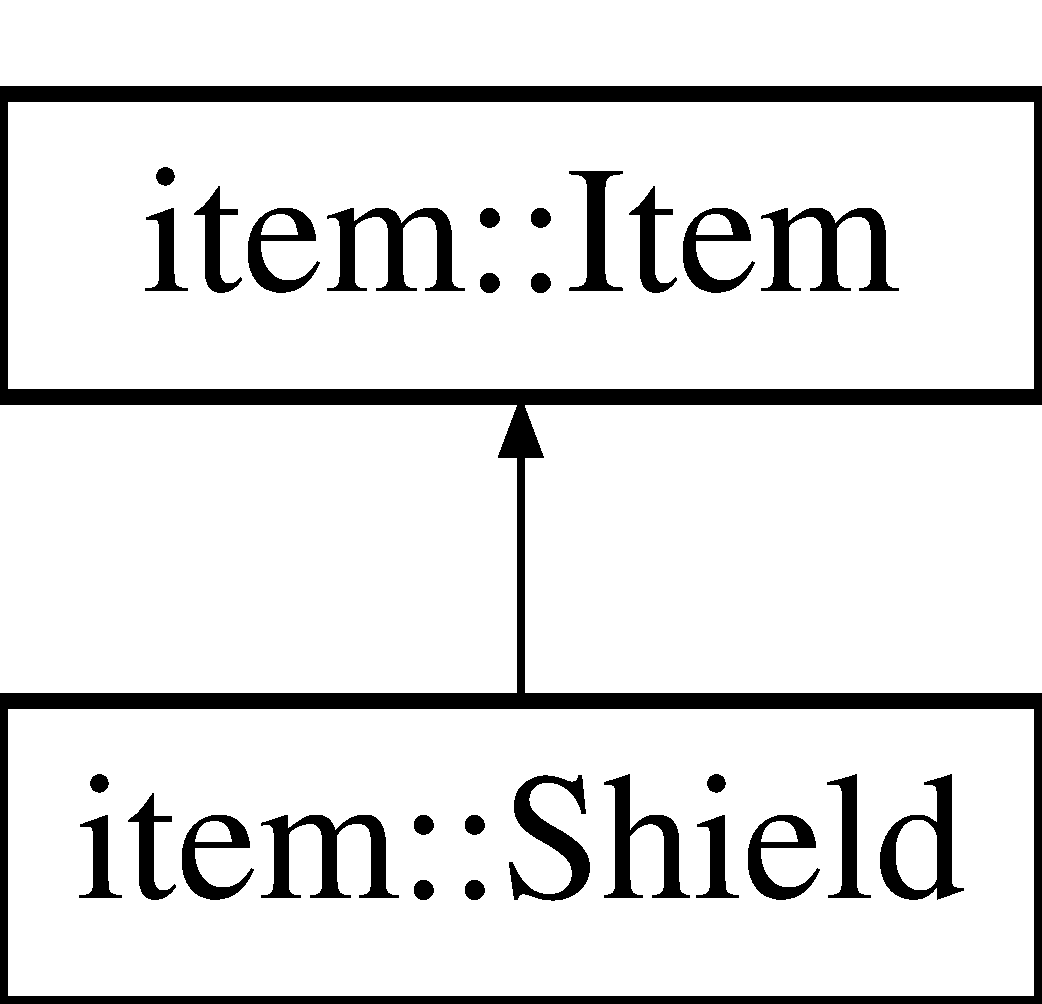
\includegraphics[height=2.000000cm]{classitem_1_1_shield}
\end{center}
\end{figure}
\subsection*{Public Member Functions}
\begin{DoxyCompactItemize}
\item 
\mbox{\Hypertarget{classitem_1_1_shield_ac65eef60e78829da35895968923fb3b7}\label{classitem_1_1_shield_ac65eef60e78829da35895968923fb3b7}} 
{\bfseries Shield} (\hyperlink{classtimeplane_1_1_moment}{Moment} first\+\_\+moment)
\item 
\hyperlink{classitem_1_1_effect}{Effect} \hyperlink{classitem_1_1_shield_abdc88bd6d0a4d6021805fa3097f47633}{View} (\hyperlink{classtimeplane_1_1_moment}{Moment} m)
\begin{DoxyCompactList}\small\item\em View the effects of an item at a specific moment. \end{DoxyCompactList}\item 
Tagged\+Values \hyperlink{classitem_1_1_shield_a1a246374ed47a4d9849bad97091c42cb}{State\+Tagged\+Values} (\hyperlink{classtimeplane_1_1_moment}{Moment} m) const
\begin{DoxyCompactList}\small\item\em Virtual method to provide user-\/friendly tagged values. \end{DoxyCompactList}\end{DoxyCompactItemize}
\subsection*{Static Public Attributes}
\begin{DoxyCompactItemize}
\item 
static Item\+Type constexpr \hyperlink{classitem_1_1_shield_a936299d37c16f407535e373f1f879d34}{type} = Item\+Type\+::k\+Shield
\begin{DoxyCompactList}\small\item\em An enum representation of the type of the item. \end{DoxyCompactList}\item 
\mbox{\Hypertarget{classitem_1_1_shield_af4d01df72cfe6f4a4b5155ba22afe2a6}\label{classitem_1_1_shield_af4d01df72cfe6f4a4b5155ba22afe2a6}} 
static int constexpr \hyperlink{classitem_1_1_shield_af4d01df72cfe6f4a4b5155ba22afe2a6}{k\+Unlock\+Requirement} = 45
\begin{DoxyCompactList}\small\item\em Energy requirement to unlock the item. \end{DoxyCompactList}\end{DoxyCompactItemize}
\subsection*{Protected Member Functions}
\begin{DoxyCompactItemize}
\item 
std\+::pair$<$ \hyperlink{classitem_1_1_effect}{Effect}, \hyperlink{classitem_1_1_item_properties}{Item\+Properties} $>$ \hyperlink{classitem_1_1_shield_a0c446c3f436c4eb221ebafd817df9a5f}{Step\+Impl} (\hyperlink{classtimeplane_1_1_moment}{Moment} curr, \hyperlink{classroundinfo_1_1_round_info_view}{Round\+Info\+View} const \&round\+\_\+info\+\_\+view, int energy\+\_\+input)
\begin{DoxyCompactList}\small\item\em Virtual method for computing the results of making a step. \end{DoxyCompactList}\item 
std\+::pair$<$ \hyperlink{classitem_1_1_effect}{Effect}, \hyperlink{classitem_1_1_item_properties}{Item\+Properties} $>$ \hyperlink{classitem_1_1_shield_a29993d7965fe391d052214cd415eec75}{Branch\+Impl} (\hyperlink{classtimeplane_1_1_moment}{Moment} curr, \hyperlink{classtimeplane_1_1_moment}{Moment} dest)
\begin{DoxyCompactList}\small\item\em Virtual method for computing the results of branching. \end{DoxyCompactList}\end{DoxyCompactItemize}
\subsection*{Additional Inherited Members}


\subsection{Detailed Description}
\hyperlink{classitem_1_1_item}{Item} that shields that player from damage. 

Shielding energy can be built up regularly, and can be transferred to the past when the player uses the \hyperlink{classitem_1_1_antitelephone}{Antitelephone}. 

\subsection{Member Function Documentation}
\mbox{\Hypertarget{classitem_1_1_shield_abdc88bd6d0a4d6021805fa3097f47633}\label{classitem_1_1_shield_abdc88bd6d0a4d6021805fa3097f47633}} 
\index{item\+::\+Shield@{item\+::\+Shield}!View@{View}}
\index{View@{View}!item\+::\+Shield@{item\+::\+Shield}}
\subsubsection{\texorpdfstring{View()}{View()}}
{\footnotesize\ttfamily \hyperlink{classitem_1_1_effect}{Effect} Shield\+::\+View (\begin{DoxyParamCaption}\item[{\hyperlink{classtimeplane_1_1_moment}{Moment}}]{m }\end{DoxyParamCaption})\hspace{0.3cm}{\ttfamily [virtual]}}



View the effects of an item at a specific moment. 


\begin{DoxyParams}{Parameters}
{\em m} & The moment to query. \\
\hline
\end{DoxyParams}
\begin{DoxyReturn}{Returns}
The effects granted by the item at the specified moment. 
\end{DoxyReturn}


Implements \hyperlink{classitem_1_1_item_a400dfeabc4056d36bfd348ff9c51cf7d}{item\+::\+Item}.

\mbox{\Hypertarget{classitem_1_1_shield_a1a246374ed47a4d9849bad97091c42cb}\label{classitem_1_1_shield_a1a246374ed47a4d9849bad97091c42cb}} 
\index{item\+::\+Shield@{item\+::\+Shield}!State\+Tagged\+Values@{State\+Tagged\+Values}}
\index{State\+Tagged\+Values@{State\+Tagged\+Values}!item\+::\+Shield@{item\+::\+Shield}}
\subsubsection{\texorpdfstring{State\+Tagged\+Values()}{StateTaggedValues()}}
{\footnotesize\ttfamily Tagged\+Values Shield\+::\+State\+Tagged\+Values (\begin{DoxyParamCaption}\item[{\hyperlink{classtimeplane_1_1_moment}{Moment}}]{m }\end{DoxyParamCaption}) const\hspace{0.3cm}{\ttfamily [virtual]}}



Virtual method to provide user-\/friendly tagged values. 

The tags are used as a user-\/friendly indication of the internal state of the item at a given moment without revealing implementation detail, and can also be used to attach specific meaning to the abstract lockdown and cooldown values associated with all items. 
\begin{DoxyParams}{Parameters}
{\em m} & The moment to query. \\
\hline
\end{DoxyParams}
\begin{DoxyReturn}{Returns}
A group of tagged values describing the state of an item. 
\end{DoxyReturn}


Implements \hyperlink{classitem_1_1_item_a8410ab3ab75e65360eddb4f6bd3cceff}{item\+::\+Item}.

\mbox{\Hypertarget{classitem_1_1_shield_a0c446c3f436c4eb221ebafd817df9a5f}\label{classitem_1_1_shield_a0c446c3f436c4eb221ebafd817df9a5f}} 
\index{item\+::\+Shield@{item\+::\+Shield}!Step\+Impl@{Step\+Impl}}
\index{Step\+Impl@{Step\+Impl}!item\+::\+Shield@{item\+::\+Shield}}
\subsubsection{\texorpdfstring{Step\+Impl()}{StepImpl()}}
{\footnotesize\ttfamily std\+::pair$<$ \hyperlink{classitem_1_1_effect}{Effect}, \hyperlink{classitem_1_1_item_properties}{Item\+Properties} $>$ Shield\+::\+Step\+Impl (\begin{DoxyParamCaption}\item[{\hyperlink{classtimeplane_1_1_moment}{Moment}}]{curr,  }\item[{\hyperlink{classroundinfo_1_1_round_info_view}{Round\+Info\+View} const \&}]{turn\+\_\+data,  }\item[{int}]{energy\+\_\+input }\end{DoxyParamCaption})\hspace{0.3cm}{\ttfamily [protected]}, {\ttfamily [virtual]}}



Virtual method for computing the results of making a step. 


\begin{DoxyParams}{Parameters}
{\em curr} & The current moment before the step. \\
\hline
{\em turn\+\_\+data} & The information about the turn just played. \\
\hline
\end{DoxyParams}
\begin{DoxyReturn}{Returns}
The effects granted by the item for the next round, and the properties of the item for the next round. 
\end{DoxyReturn}


Implements \hyperlink{classitem_1_1_item_a90df61c8a2a20144eb1100af5fb2d464}{item\+::\+Item}.

\mbox{\Hypertarget{classitem_1_1_shield_a29993d7965fe391d052214cd415eec75}\label{classitem_1_1_shield_a29993d7965fe391d052214cd415eec75}} 
\index{item\+::\+Shield@{item\+::\+Shield}!Branch\+Impl@{Branch\+Impl}}
\index{Branch\+Impl@{Branch\+Impl}!item\+::\+Shield@{item\+::\+Shield}}
\subsubsection{\texorpdfstring{Branch\+Impl()}{BranchImpl()}}
{\footnotesize\ttfamily std\+::pair$<$ \hyperlink{classitem_1_1_effect}{Effect}, \hyperlink{classitem_1_1_item_properties}{Item\+Properties} $>$ Shield\+::\+Branch\+Impl (\begin{DoxyParamCaption}\item[{\hyperlink{classtimeplane_1_1_moment}{Moment}}]{curr,  }\item[{\hyperlink{classtimeplane_1_1_moment}{Moment}}]{dest }\end{DoxyParamCaption})\hspace{0.3cm}{\ttfamily [protected]}, {\ttfamily [virtual]}}



Virtual method for computing the results of branching. 


\begin{DoxyParams}{Parameters}
{\em curr} & The current moment before branching. \\
\hline
{\em dest} & The destination moment to reach. \\
\hline
\end{DoxyParams}
\begin{DoxyReturn}{Returns}
The effects granted by the item for the next round, and the properties of the item for the next round. 
\end{DoxyReturn}


Implements \hyperlink{classitem_1_1_item_afef6bdd5c1c734c67122e4118e9e1930}{item\+::\+Item}.



\subsection{Member Data Documentation}
\mbox{\Hypertarget{classitem_1_1_shield_a936299d37c16f407535e373f1f879d34}\label{classitem_1_1_shield_a936299d37c16f407535e373f1f879d34}} 
\index{item\+::\+Shield@{item\+::\+Shield}!type@{type}}
\index{type@{type}!item\+::\+Shield@{item\+::\+Shield}}
\subsubsection{\texorpdfstring{type}{type}}
{\footnotesize\ttfamily Item\+Type constexpr item\+::\+Shield\+::type = Item\+Type\+::k\+Shield\hspace{0.3cm}{\ttfamily [static]}}



An enum representation of the type of the item. 

The value of the enum is a unique value for each item, and are consecutive starting at 0 across all items. 

The documentation for this class was generated from the following files\+:\begin{DoxyCompactItemize}
\item 
K\+:/\+Personal Projects/\+Antitelephone\+Q\+T/src/shield.\+hpp\item 
K\+:/\+Personal Projects/\+Antitelephone\+Q\+T/src/shield.\+cpp\end{DoxyCompactItemize}

\hypertarget{class_symmetric_bit_matrix}{}\section{Symmetric\+Bit\+Matrix Class Reference}
\label{class_symmetric_bit_matrix}\index{Symmetric\+Bit\+Matrix@{Symmetric\+Bit\+Matrix}}


A symmetric square matrix of boolean values.  




{\ttfamily \#include $<$symmetricbitmatrix.\+hpp$>$}

\subsection*{Public Member Functions}
\begin{DoxyCompactItemize}
\item 
\hyperlink{class_symmetric_bit_matrix_a828dbcd597cd13390922d863357da3f3}{Symmetric\+Bit\+Matrix} (int \hyperlink{class_symmetric_bit_matrix_aed948744d70716f6325063ed55a76c6c}{size})
\begin{DoxyCompactList}\small\item\em Constructor. \end{DoxyCompactList}\item 
int \hyperlink{class_symmetric_bit_matrix_aed948744d70716f6325063ed55a76c6c}{size} () const noexcept
\begin{DoxyCompactList}\small\item\em Accessor for the size of the matrix. \end{DoxyCompactList}\item 
bool \hyperlink{class_symmetric_bit_matrix_a02221e8620c41734a56ec329da1b66c6}{Value} (int row, int col) const
\begin{DoxyCompactList}\small\item\em Accessor for a boolean value at a specific position. \end{DoxyCompactList}\item 
void \hyperlink{class_symmetric_bit_matrix_a5d97dfec2cf3910b2f46b80307528c43}{Set\+Value} (int row, int col, bool value)
\begin{DoxyCompactList}\small\item\em Mutator for a boolean value at a specific position. \end{DoxyCompactList}\end{DoxyCompactItemize}


\subsection{Detailed Description}
A symmetric square matrix of boolean values. 

\subsection{Constructor \& Destructor Documentation}
\mbox{\Hypertarget{class_symmetric_bit_matrix_a828dbcd597cd13390922d863357da3f3}\label{class_symmetric_bit_matrix_a828dbcd597cd13390922d863357da3f3}} 
\index{Symmetric\+Bit\+Matrix@{Symmetric\+Bit\+Matrix}!Symmetric\+Bit\+Matrix@{Symmetric\+Bit\+Matrix}}
\index{Symmetric\+Bit\+Matrix@{Symmetric\+Bit\+Matrix}!Symmetric\+Bit\+Matrix@{Symmetric\+Bit\+Matrix}}
\subsubsection{\texorpdfstring{Symmetric\+Bit\+Matrix()}{SymmetricBitMatrix()}}
{\footnotesize\ttfamily Symmetric\+Bit\+Matrix\+::\+Symmetric\+Bit\+Matrix (\begin{DoxyParamCaption}\item[{int}]{size }\end{DoxyParamCaption})\hspace{0.3cm}{\ttfamily [inline]}}



Constructor. 

The boolean values are by default all set to {\ttfamily false}. 
\begin{DoxyParams}{Parameters}
{\em size} & The dimensions of the matrix to create. \\
\hline
\end{DoxyParams}


\subsection{Member Function Documentation}
\mbox{\Hypertarget{class_symmetric_bit_matrix_aed948744d70716f6325063ed55a76c6c}\label{class_symmetric_bit_matrix_aed948744d70716f6325063ed55a76c6c}} 
\index{Symmetric\+Bit\+Matrix@{Symmetric\+Bit\+Matrix}!size@{size}}
\index{size@{size}!Symmetric\+Bit\+Matrix@{Symmetric\+Bit\+Matrix}}
\subsubsection{\texorpdfstring{size()}{size()}}
{\footnotesize\ttfamily int Symmetric\+Bit\+Matrix\+::size (\begin{DoxyParamCaption}{ }\end{DoxyParamCaption}) const\hspace{0.3cm}{\ttfamily [inline]}, {\ttfamily [noexcept]}}



Accessor for the size of the matrix. 

\begin{DoxyReturn}{Returns}
The number of rows, or number of columns in the matrix. 
\end{DoxyReturn}
\mbox{\Hypertarget{class_symmetric_bit_matrix_a02221e8620c41734a56ec329da1b66c6}\label{class_symmetric_bit_matrix_a02221e8620c41734a56ec329da1b66c6}} 
\index{Symmetric\+Bit\+Matrix@{Symmetric\+Bit\+Matrix}!Value@{Value}}
\index{Value@{Value}!Symmetric\+Bit\+Matrix@{Symmetric\+Bit\+Matrix}}
\subsubsection{\texorpdfstring{Value()}{Value()}}
{\footnotesize\ttfamily bool Symmetric\+Bit\+Matrix\+::\+Value (\begin{DoxyParamCaption}\item[{int}]{row,  }\item[{int}]{col }\end{DoxyParamCaption}) const\hspace{0.3cm}{\ttfamily [inline]}}



Accessor for a boolean value at a specific position. 


\begin{DoxyParams}{Parameters}
{\em row} & The row to query. \\
\hline
{\em col} & The column to query. \\
\hline
\end{DoxyParams}
\begin{DoxyReturn}{Returns}
The boolean value at the specified position. 
\end{DoxyReturn}
\mbox{\Hypertarget{class_symmetric_bit_matrix_a5d97dfec2cf3910b2f46b80307528c43}\label{class_symmetric_bit_matrix_a5d97dfec2cf3910b2f46b80307528c43}} 
\index{Symmetric\+Bit\+Matrix@{Symmetric\+Bit\+Matrix}!Set\+Value@{Set\+Value}}
\index{Set\+Value@{Set\+Value}!Symmetric\+Bit\+Matrix@{Symmetric\+Bit\+Matrix}}
\subsubsection{\texorpdfstring{Set\+Value()}{SetValue()}}
{\footnotesize\ttfamily void Symmetric\+Bit\+Matrix\+::\+Set\+Value (\begin{DoxyParamCaption}\item[{int}]{row,  }\item[{int}]{col,  }\item[{bool}]{value }\end{DoxyParamCaption})\hspace{0.3cm}{\ttfamily [inline]}}



Mutator for a boolean value at a specific position. 


\begin{DoxyParams}{Parameters}
{\em row} & The row to set. \\
\hline
{\em col} & The column to set. \\
\hline
{\em value} & The boolean value to set. \\
\hline
\end{DoxyParams}


The documentation for this class was generated from the following file\+:\begin{DoxyCompactItemize}
\item 
K\+:/\+Personal Projects/\+Antitelephone\+Q\+T/src/symmetricbitmatrix.\+hpp\end{DoxyCompactItemize}

\hypertarget{classtimeplane_1_1_time_line}{}\section{timeplane\+:\+:Time\+Line Class Reference}
\label{classtimeplane_1_1_time_line}\index{timeplane\+::\+Time\+Line@{timeplane\+::\+Time\+Line}}


A chronological sequence of {\ttfamily \hyperlink{classtimeplane_1_1_moment}{Moment}} instances.  




{\ttfamily \#include $<$timeline.\+hpp$>$}

\subsection*{Public Types}
\begin{DoxyCompactItemize}
\item 
\mbox{\Hypertarget{classtimeplane_1_1_time_line_a6f6445b9dc0cafb2affc5f146aa2d5c9}\label{classtimeplane_1_1_time_line_a6f6445b9dc0cafb2affc5f146aa2d5c9}} 
using {\bfseries Moment\+Iterators} = \+::std\+::pair$<$\+::std\+::vector$<$ \hyperlink{classtimeplane_1_1_moment}{Moment} $>$\+::iterator, \+::std\+::vector$<$ \hyperlink{classtimeplane_1_1_moment}{Moment} $>$\+::iterator $>$
\item 
\mbox{\Hypertarget{classtimeplane_1_1_time_line_ac0192758efee9819ae91308d339fc3f4}\label{classtimeplane_1_1_time_line_ac0192758efee9819ae91308d339fc3f4}} 
using {\bfseries Moment\+Deleter} = \+::std\+::function$<$ void(typename Moment\+Iterators)$>$
\end{DoxyCompactItemize}
\subsection*{Public Member Functions}
\begin{DoxyCompactItemize}
\item 
\hyperlink{classtimeplane_1_1_time_line_afacd08f817ddae17b1dea9c1989f74ae}{Time\+Line} (Moment\+Deleter moment\+\_\+deleter=Moment\+Deleter\{\})
\begin{DoxyCompactList}\small\item\em Default constructor. \end{DoxyCompactList}\item 
\hyperlink{classtimeplane_1_1_time_line_a5e9a864bc9838c82dc3e5a50e69ece9b}{Time\+Line} (\hyperlink{classtimeplane_1_1_time_line}{Time\+Line} const \&left\+\_\+timeline, int branch\+\_\+time, Moment\+Deleter moment\+\_\+deleter=Moment\+Deleter\{\})
\begin{DoxyCompactList}\small\item\em Constructor from an existing timeline. \end{DoxyCompactList}\item 
\hyperlink{classtimeplane_1_1_time_line_a2d16c3db644a5e8dc4c0f12622c6a4e6}{$\sim$\+Time\+Line} ()
\begin{DoxyCompactList}\small\item\em Destructor. \end{DoxyCompactList}\item 
int const \hyperlink{classtimeplane_1_1_time_line_a4297da8acc6fbee73bfc7db0de2f80a5}{timeline\+\_\+number} () const noexcept
\begin{DoxyCompactList}\small\item\em Accessor for the timeline number. \end{DoxyCompactList}\item 
\hyperlink{classtimeplane_1_1_moment}{Moment} const \hyperlink{classtimeplane_1_1_time_line_ae18ca86c0f036731e1bb148ed3381ea8}{Get\+Moment} (int time) const
\begin{DoxyCompactList}\small\item\em Accesses the moment with the specified time. \end{DoxyCompactList}\item 
\hyperlink{classtimeplane_1_1_moment}{Moment} const \hyperlink{classtimeplane_1_1_time_line_a7520362a8b33962371b1a47831b37b03}{Make\+Moment} ()
\begin{DoxyCompactList}\small\item\em Creates a new moment at the end of the timeline. \end{DoxyCompactList}\item 
\hyperlink{classtimeplane_1_1_moment}{Moment} const \hyperlink{classtimeplane_1_1_time_line_acc391553e5c45a647c82f27e53ae3af8}{Latest\+Moment} () const noexcept
\begin{DoxyCompactList}\small\item\em Retrieve the latest moment from the timeline. \end{DoxyCompactList}\item 
\mbox{\Hypertarget{classtimeplane_1_1_time_line_abba50bd707ce998356abd59bbf302f94}\label{classtimeplane_1_1_time_line_abba50bd707ce998356abd59bbf302f94}} 
{\bfseries Time\+Line} (\hyperlink{classtimeplane_1_1_time_line}{Time\+Line} const \&)=delete
\item 
\mbox{\Hypertarget{classtimeplane_1_1_time_line_ad8eb0c4a4c85e5d859fab5e1d70a757f}\label{classtimeplane_1_1_time_line_ad8eb0c4a4c85e5d859fab5e1d70a757f}} 
\hyperlink{classtimeplane_1_1_time_line}{Time\+Line} \& {\bfseries operator=} (\hyperlink{classtimeplane_1_1_time_line}{Time\+Line} const \&)=delete
\item 
\mbox{\Hypertarget{classtimeplane_1_1_time_line_a345833bfe7d67e2ca39067e92cb4929a}\label{classtimeplane_1_1_time_line_a345833bfe7d67e2ca39067e92cb4929a}} 
{\bfseries Time\+Line} (\hyperlink{classtimeplane_1_1_time_line}{Time\+Line} \&\&)=default
\item 
\mbox{\Hypertarget{classtimeplane_1_1_time_line_a6914130bc8b7bed844517bd0daed7b6b}\label{classtimeplane_1_1_time_line_a6914130bc8b7bed844517bd0daed7b6b}} 
\hyperlink{classtimeplane_1_1_time_line}{Time\+Line} \& {\bfseries operator=} (\hyperlink{classtimeplane_1_1_time_line}{Time\+Line} \&\&)=default
\end{DoxyCompactItemize}


\subsection{Detailed Description}
A chronological sequence of {\ttfamily \hyperlink{classtimeplane_1_1_moment}{Moment}} instances. 

The times of the {\ttfamily \hyperlink{classtimeplane_1_1_moment}{Moment}} instances in a timeline are consecutive and begin at 0. It is possible to create new moments at the end of the timeline or retrieve moments at any valid time in the timeline. 

\subsection{Constructor \& Destructor Documentation}
\mbox{\Hypertarget{classtimeplane_1_1_time_line_afacd08f817ddae17b1dea9c1989f74ae}\label{classtimeplane_1_1_time_line_afacd08f817ddae17b1dea9c1989f74ae}} 
\index{timeplane\+::\+Time\+Line@{timeplane\+::\+Time\+Line}!Time\+Line@{Time\+Line}}
\index{Time\+Line@{Time\+Line}!timeplane\+::\+Time\+Line@{timeplane\+::\+Time\+Line}}
\subsubsection{\texorpdfstring{Time\+Line()}{TimeLine()}\hspace{0.1cm}{\footnotesize\ttfamily [1/2]}}
{\footnotesize\ttfamily timeplane\+::\+Time\+Line\+::\+Time\+Line (\begin{DoxyParamCaption}\item[{Moment\+Deleter}]{moment\+\_\+deleter = {\ttfamily MomentDeleter\{\}} }\end{DoxyParamCaption})}



Default constructor. 

This constructor is used to make the leftmost timeline, and in the process it creates the earliest moment as well. 
\begin{DoxyParams}{Parameters}
{\em moment\+\_\+deleter} & A handler for moments that fall out of scope from outside clients. \\
\hline
\end{DoxyParams}
\mbox{\Hypertarget{classtimeplane_1_1_time_line_a5e9a864bc9838c82dc3e5a50e69ece9b}\label{classtimeplane_1_1_time_line_a5e9a864bc9838c82dc3e5a50e69ece9b}} 
\index{timeplane\+::\+Time\+Line@{timeplane\+::\+Time\+Line}!Time\+Line@{Time\+Line}}
\index{Time\+Line@{Time\+Line}!timeplane\+::\+Time\+Line@{timeplane\+::\+Time\+Line}}
\subsubsection{\texorpdfstring{Time\+Line()}{TimeLine()}\hspace{0.1cm}{\footnotesize\ttfamily [2/2]}}
{\footnotesize\ttfamily timeplane\+::\+Time\+Line\+::\+Time\+Line (\begin{DoxyParamCaption}\item[{\hyperlink{classtimeplane_1_1_time_line}{Time\+Line} const \&}]{left\+\_\+timeline,  }\item[{int}]{branch\+\_\+time,  }\item[{Moment\+Deleter}]{moment\+\_\+deleter = {\ttfamily MomentDeleter\{\}} }\end{DoxyParamCaption})}



Constructor from an existing timeline. 

This constructor creates a timeline as a branch of an existing timeline. It also creates a distinct {\ttfamily \hyperlink{classtimeplane_1_1_moment}{Moment}} instance in the newly created timeline whose time is equal to the branch time. 
\begin{DoxyParams}{Parameters}
{\em left\+\_\+timeline} & The timeline to branch from. \\
\hline
{\em branch\+\_\+time} & The time to branch off from. \\
\hline
{\em moment\+\_\+deleter} & A handler for moments that fall out of scope from outside clients. \\
\hline
\end{DoxyParams}
\mbox{\Hypertarget{classtimeplane_1_1_time_line_a2d16c3db644a5e8dc4c0f12622c6a4e6}\label{classtimeplane_1_1_time_line_a2d16c3db644a5e8dc4c0f12622c6a4e6}} 
\index{timeplane\+::\+Time\+Line@{timeplane\+::\+Time\+Line}!````~Time\+Line@{$\sim$\+Time\+Line}}
\index{````~Time\+Line@{$\sim$\+Time\+Line}!timeplane\+::\+Time\+Line@{timeplane\+::\+Time\+Line}}
\subsubsection{\texorpdfstring{$\sim$\+Time\+Line()}{~TimeLine()}}
{\footnotesize\ttfamily timeplane\+::\+Time\+Line\+::$\sim$\+Time\+Line (\begin{DoxyParamCaption}{ }\end{DoxyParamCaption})}



Destructor. 

The moment deletion handler, if active, is called to handle the removal of all moments contained within the timeline before it is destroyed. 

\subsection{Member Function Documentation}
\mbox{\Hypertarget{classtimeplane_1_1_time_line_ae18ca86c0f036731e1bb148ed3381ea8}\label{classtimeplane_1_1_time_line_ae18ca86c0f036731e1bb148ed3381ea8}} 
\index{timeplane\+::\+Time\+Line@{timeplane\+::\+Time\+Line}!Get\+Moment@{Get\+Moment}}
\index{Get\+Moment@{Get\+Moment}!timeplane\+::\+Time\+Line@{timeplane\+::\+Time\+Line}}
\subsubsection{\texorpdfstring{Get\+Moment()}{GetMoment()}}
{\footnotesize\ttfamily \hyperlink{classtimeplane_1_1_moment}{Moment} const timeplane\+::\+Time\+Line\+::\+Get\+Moment (\begin{DoxyParamCaption}\item[{int}]{time }\end{DoxyParamCaption}) const}



Accesses the moment with the specified time. 


\begin{DoxyParams}{Parameters}
{\em time} & The time to query. \\
\hline
\end{DoxyParams}
\begin{DoxyReturn}{Returns}
The {\ttfamily \hyperlink{classtimeplane_1_1_moment}{Moment}} instance at the specified time. 
\end{DoxyReturn}

\begin{DoxyExceptions}{Exceptions}
{\em std\+::out\+\_\+of\+\_\+range} & If no moment exists at the specified time. \\
\hline
\end{DoxyExceptions}
\mbox{\Hypertarget{classtimeplane_1_1_time_line_acc391553e5c45a647c82f27e53ae3af8}\label{classtimeplane_1_1_time_line_acc391553e5c45a647c82f27e53ae3af8}} 
\index{timeplane\+::\+Time\+Line@{timeplane\+::\+Time\+Line}!Latest\+Moment@{Latest\+Moment}}
\index{Latest\+Moment@{Latest\+Moment}!timeplane\+::\+Time\+Line@{timeplane\+::\+Time\+Line}}
\subsubsection{\texorpdfstring{Latest\+Moment()}{LatestMoment()}}
{\footnotesize\ttfamily \hyperlink{classtimeplane_1_1_moment}{Moment} const timeplane\+::\+Time\+Line\+::\+Latest\+Moment (\begin{DoxyParamCaption}{ }\end{DoxyParamCaption}) const\hspace{0.3cm}{\ttfamily [noexcept]}}



Retrieve the latest moment from the timeline. 

\begin{DoxyReturn}{Returns}
The moment at the end of the timeline. 
\end{DoxyReturn}
\mbox{\Hypertarget{classtimeplane_1_1_time_line_a7520362a8b33962371b1a47831b37b03}\label{classtimeplane_1_1_time_line_a7520362a8b33962371b1a47831b37b03}} 
\index{timeplane\+::\+Time\+Line@{timeplane\+::\+Time\+Line}!Make\+Moment@{Make\+Moment}}
\index{Make\+Moment@{Make\+Moment}!timeplane\+::\+Time\+Line@{timeplane\+::\+Time\+Line}}
\subsubsection{\texorpdfstring{Make\+Moment()}{MakeMoment()}}
{\footnotesize\ttfamily \hyperlink{classtimeplane_1_1_moment}{Moment} const timeplane\+::\+Time\+Line\+::\+Make\+Moment (\begin{DoxyParamCaption}{ }\end{DoxyParamCaption})}



Creates a new moment at the end of the timeline. 

\begin{DoxyReturn}{Returns}
The moment newly created. 
\end{DoxyReturn}
\mbox{\Hypertarget{classtimeplane_1_1_time_line_a4297da8acc6fbee73bfc7db0de2f80a5}\label{classtimeplane_1_1_time_line_a4297da8acc6fbee73bfc7db0de2f80a5}} 
\index{timeplane\+::\+Time\+Line@{timeplane\+::\+Time\+Line}!timeline\+\_\+number@{timeline\+\_\+number}}
\index{timeline\+\_\+number@{timeline\+\_\+number}!timeplane\+::\+Time\+Line@{timeplane\+::\+Time\+Line}}
\subsubsection{\texorpdfstring{timeline\+\_\+number()}{timeline\_number()}}
{\footnotesize\ttfamily int const timeplane\+::\+Time\+Line\+::timeline\+\_\+number (\begin{DoxyParamCaption}{ }\end{DoxyParamCaption}) const\hspace{0.3cm}{\ttfamily [noexcept]}}



Accessor for the timeline number. 

\begin{DoxyReturn}{Returns}
An ID number unique to a timeline. 
\end{DoxyReturn}


The documentation for this class was generated from the following file\+:\begin{DoxyCompactItemize}
\item 
K\+:/\+Personal Projects/\+Antitelephone\+Q\+T/src/timeline.\+hpp\end{DoxyCompactItemize}

\hypertarget{classtimeplane_1_1_time_plane}{}\section{timeplane\+:\+:Time\+Plane Class Reference}
\label{classtimeplane_1_1_time_plane}\index{timeplane\+::\+Time\+Plane@{timeplane\+::\+Time\+Plane}}


A wrapper to access individual {\ttfamily \hyperlink{classtimeplane_1_1_time_line}{Time\+Line}} instances.  




{\ttfamily \#include $<$timeplane.\+hpp$>$}

\subsection*{Public Member Functions}
\begin{DoxyCompactItemize}
\item 
\hyperlink{classtimeplane_1_1_time_plane_a8d8f1227ade6490fa8b814f1b7f18ecc}{Time\+Plane} ()
\begin{DoxyCompactList}\small\item\em Default constructor. \end{DoxyCompactList}\item 
int \hyperlink{classtimeplane_1_1_time_plane_ae66d15a7ce9adb5f63906011a455400b}{latest\+\_\+antitelephone\+\_\+arrival} () const noexcept
\begin{DoxyCompactList}\small\item\em Accessor for the latest Antitelephone arrival time. \end{DoxyCompactList}\item 
\hyperlink{classtimeplane_1_1_time_line}{Time\+Line} \& \hyperlink{classtimeplane_1_1_time_plane_a317c9e247011cf5f4e6e36f2f7651932}{rightmost\+\_\+timeline} () noexcept
\begin{DoxyCompactList}\small\item\em Accessor for the rightmost timeline. \end{DoxyCompactList}\item 
boost\+::optional$<$ \hyperlink{classtimeplane_1_1_time_line}{Time\+Line} $>$ \& \hyperlink{classtimeplane_1_1_time_plane_a32da05c87dfe4bc33ec5cb87fd97297f}{second\+\_\+rightmost\+\_\+time\+Line} () noexcept
\begin{DoxyCompactList}\small\item\em Accessor for the rightmost timeline. \end{DoxyCompactList}\item 
\hyperlink{classtimeplane_1_1_time_line}{Time\+Line} \& \hyperlink{classtimeplane_1_1_time_plane_ab8c82092c1c5c3f18c8677f8ce38662c}{Make\+New\+Time\+Line} (int branch\+\_\+time)
\begin{DoxyCompactList}\small\item\em Creates a new timeline branching from the rightmost timeline. \end{DoxyCompactList}\item 
void \hyperlink{classtimeplane_1_1_time_plane_a10f6e26c2043a2d2cb0271a06c2495d0}{Register\+Moment\+Deleter} (Moment\+Deleter handler)
\begin{DoxyCompactList}\small\item\em Registers a moment deletion handler. \end{DoxyCompactList}\end{DoxyCompactItemize}
\subsection*{Static Public Attributes}
\begin{DoxyCompactItemize}
\item 
\mbox{\Hypertarget{classtimeplane_1_1_time_plane_ab131bfc5a6c85a3db846591159db2559}\label{classtimeplane_1_1_time_plane_ab131bfc5a6c85a3db846591159db2559}} 
static constexpr int \hyperlink{classtimeplane_1_1_time_plane_ab131bfc5a6c85a3db846591159db2559}{k\+No\+Antitelephone\+Arrival} = -\/1
\begin{DoxyCompactList}\small\item\em Constant representing a lack of antitelephone arrivals. \end{DoxyCompactList}\end{DoxyCompactItemize}


\subsection{Detailed Description}
A wrapper to access individual {\ttfamily \hyperlink{classtimeplane_1_1_time_line}{Time\+Line}} instances. 

A timeplane can logically be thought of as a sequence of linearly connected timelines spanning left to right (where time flows upward within each timeline). Currently the class allows access to the rightmost and second-\/rightmost timelines only. The user can register handlers to clean up their data structures whenever any {\ttfamily \hyperlink{classtimeplane_1_1_moment}{Moment}} instances are no longer externally accessible. 

\subsection{Constructor \& Destructor Documentation}
\mbox{\Hypertarget{classtimeplane_1_1_time_plane_a8d8f1227ade6490fa8b814f1b7f18ecc}\label{classtimeplane_1_1_time_plane_a8d8f1227ade6490fa8b814f1b7f18ecc}} 
\index{timeplane\+::\+Time\+Plane@{timeplane\+::\+Time\+Plane}!Time\+Plane@{Time\+Plane}}
\index{Time\+Plane@{Time\+Plane}!timeplane\+::\+Time\+Plane@{timeplane\+::\+Time\+Plane}}
\subsubsection{\texorpdfstring{Time\+Plane()}{TimePlane()}}
{\footnotesize\ttfamily Time\+Plane\+::\+Time\+Plane (\begin{DoxyParamCaption}{ }\end{DoxyParamCaption})}



Default constructor. 

A single timeline is created and within it, a single moment is also created. 

\subsection{Member Function Documentation}
\mbox{\Hypertarget{classtimeplane_1_1_time_plane_ae66d15a7ce9adb5f63906011a455400b}\label{classtimeplane_1_1_time_plane_ae66d15a7ce9adb5f63906011a455400b}} 
\index{timeplane\+::\+Time\+Plane@{timeplane\+::\+Time\+Plane}!latest\+\_\+antitelephone\+\_\+arrival@{latest\+\_\+antitelephone\+\_\+arrival}}
\index{latest\+\_\+antitelephone\+\_\+arrival@{latest\+\_\+antitelephone\+\_\+arrival}!timeplane\+::\+Time\+Plane@{timeplane\+::\+Time\+Plane}}
\subsubsection{\texorpdfstring{latest\+\_\+antitelephone\+\_\+arrival()}{latest\_antitelephone\_arrival()}}
{\footnotesize\ttfamily int timeplane\+::\+Time\+Plane\+::latest\+\_\+antitelephone\+\_\+arrival (\begin{DoxyParamCaption}{ }\end{DoxyParamCaption}) const\hspace{0.3cm}{\ttfamily [inline]}, {\ttfamily [noexcept]}}



Accessor for the latest Antitelephone arrival time. 

The value applies to the rightmost timeline, though note that Antitelephone arrivals all still occur for timelines to the right of the leftmost arrival, even if some of these timelines have early Antitelephone arrivals.

If there is no Antitelephone arrival, then the constant {\ttfamily k\+No\+Antitelephone\+Arrival} is returned. \begin{DoxyReturn}{Returns}
Time of the latest Antitelephone arrival. 
\end{DoxyReturn}
\mbox{\Hypertarget{classtimeplane_1_1_time_plane_ab8c82092c1c5c3f18c8677f8ce38662c}\label{classtimeplane_1_1_time_plane_ab8c82092c1c5c3f18c8677f8ce38662c}} 
\index{timeplane\+::\+Time\+Plane@{timeplane\+::\+Time\+Plane}!Make\+New\+Time\+Line@{Make\+New\+Time\+Line}}
\index{Make\+New\+Time\+Line@{Make\+New\+Time\+Line}!timeplane\+::\+Time\+Plane@{timeplane\+::\+Time\+Plane}}
\subsubsection{\texorpdfstring{Make\+New\+Time\+Line()}{MakeNewTimeLine()}}
{\footnotesize\ttfamily \hyperlink{classtimeplane_1_1_time_line}{Time\+Line} \& Time\+Plane\+::\+Make\+New\+Time\+Line (\begin{DoxyParamCaption}\item[{int}]{branch\+\_\+time }\end{DoxyParamCaption})}



Creates a new timeline branching from the rightmost timeline. 

The reference returned is invalidated once a new timeline is created. 
\begin{DoxyParams}{Parameters}
{\em branch\+\_\+time} & The time of the branch, which will be the the time of the sole moment available in the new timeline. \\
\hline
\end{DoxyParams}
\begin{DoxyReturn}{Returns}
A reference to the newly created timeline. 
\end{DoxyReturn}
\mbox{\Hypertarget{classtimeplane_1_1_time_plane_a10f6e26c2043a2d2cb0271a06c2495d0}\label{classtimeplane_1_1_time_plane_a10f6e26c2043a2d2cb0271a06c2495d0}} 
\index{timeplane\+::\+Time\+Plane@{timeplane\+::\+Time\+Plane}!Register\+Moment\+Deleter@{Register\+Moment\+Deleter}}
\index{Register\+Moment\+Deleter@{Register\+Moment\+Deleter}!timeplane\+::\+Time\+Plane@{timeplane\+::\+Time\+Plane}}
\subsubsection{\texorpdfstring{Register\+Moment\+Deleter()}{RegisterMomentDeleter()}}
{\footnotesize\ttfamily void timeplane\+::\+Time\+Plane\+::\+Register\+Moment\+Deleter (\begin{DoxyParamCaption}\item[{Moment\+Deleter}]{handler }\end{DoxyParamCaption})\hspace{0.3cm}{\ttfamily [inline]}}



Registers a moment deletion handler. 

The moment deletion handler is called with a pair of output iterators denoting {\ttfamily \hyperlink{classtimeplane_1_1_moment}{Moment}} instances that are no longer externally accessible. 
\begin{DoxyParams}{Parameters}
{\em handler} & The moment deletion handler to register. \\
\hline
\end{DoxyParams}
\mbox{\Hypertarget{classtimeplane_1_1_time_plane_a317c9e247011cf5f4e6e36f2f7651932}\label{classtimeplane_1_1_time_plane_a317c9e247011cf5f4e6e36f2f7651932}} 
\index{timeplane\+::\+Time\+Plane@{timeplane\+::\+Time\+Plane}!rightmost\+\_\+timeline@{rightmost\+\_\+timeline}}
\index{rightmost\+\_\+timeline@{rightmost\+\_\+timeline}!timeplane\+::\+Time\+Plane@{timeplane\+::\+Time\+Plane}}
\subsubsection{\texorpdfstring{rightmost\+\_\+timeline()}{rightmost\_timeline()}}
{\footnotesize\ttfamily \hyperlink{classtimeplane_1_1_time_line}{Time\+Line}\& timeplane\+::\+Time\+Plane\+::rightmost\+\_\+timeline (\begin{DoxyParamCaption}{ }\end{DoxyParamCaption})\hspace{0.3cm}{\ttfamily [inline]}, {\ttfamily [noexcept]}}



Accessor for the rightmost timeline. 

The reference returned is invalidated once a new timeline is created. \begin{DoxyReturn}{Returns}
A reference to the rightmost timeline. 
\end{DoxyReturn}
\mbox{\Hypertarget{classtimeplane_1_1_time_plane_a32da05c87dfe4bc33ec5cb87fd97297f}\label{classtimeplane_1_1_time_plane_a32da05c87dfe4bc33ec5cb87fd97297f}} 
\index{timeplane\+::\+Time\+Plane@{timeplane\+::\+Time\+Plane}!second\+\_\+rightmost\+\_\+time\+Line@{second\+\_\+rightmost\+\_\+time\+Line}}
\index{second\+\_\+rightmost\+\_\+time\+Line@{second\+\_\+rightmost\+\_\+time\+Line}!timeplane\+::\+Time\+Plane@{timeplane\+::\+Time\+Plane}}
\subsubsection{\texorpdfstring{second\+\_\+rightmost\+\_\+time\+Line()}{second\_rightmost\_timeLine()}}
{\footnotesize\ttfamily boost\+::optional$<$\hyperlink{classtimeplane_1_1_time_line}{Time\+Line}$>$\& timeplane\+::\+Time\+Plane\+::second\+\_\+rightmost\+\_\+time\+Line (\begin{DoxyParamCaption}{ }\end{DoxyParamCaption})\hspace{0.3cm}{\ttfamily [inline]}, {\ttfamily [noexcept]}}



Accessor for the rightmost timeline. 

The reference returned is invalidated once a new timeline is created. \begin{DoxyReturn}{Returns}
A reference to an optional type containing the rightmost timeline, or {\ttfamily boost\+::none} if there is no such timeline. 
\end{DoxyReturn}


The documentation for this class was generated from the following files\+:\begin{DoxyCompactItemize}
\item 
K\+:/\+Personal Projects/\+Antitelephone\+Q\+T/src/timeplane.\+hpp\item 
K\+:/\+Personal Projects/\+Antitelephone\+Q\+T/src/timeplane.\+cpp\end{DoxyCompactItemize}

%--- End generated contents ---

% Index
\backmatter
\newpage
\phantomsection
\clearemptydoublepage
\addcontentsline{toc}{chapter}{Index}
\printindex

\end{document}
